% Options for packages loaded elsewhere
\PassOptionsToPackage{unicode}{hyperref}
\PassOptionsToPackage{hyphens}{url}
%
\documentclass[
]{article}
\usepackage{amsmath,amssymb}
\usepackage{iftex}
\ifPDFTeX
  \usepackage[T1]{fontenc}
  \usepackage[utf8]{inputenc}
  \usepackage{textcomp} % provide euro and other symbols
\else % if luatex or xetex
  \usepackage{unicode-math} % this also loads fontspec
  \defaultfontfeatures{Scale=MatchLowercase}
  \defaultfontfeatures[\rmfamily]{Ligatures=TeX,Scale=1}
\fi
\usepackage{lmodern}
\ifPDFTeX\else
  % xetex/luatex font selection
\fi
% Use upquote if available, for straight quotes in verbatim environments
\IfFileExists{upquote.sty}{\usepackage{upquote}}{}
\IfFileExists{microtype.sty}{% use microtype if available
  \usepackage[]{microtype}
  \UseMicrotypeSet[protrusion]{basicmath} % disable protrusion for tt fonts
}{}
\makeatletter
\@ifundefined{KOMAClassName}{% if non-KOMA class
  \IfFileExists{parskip.sty}{%
    \usepackage{parskip}
  }{% else
    \setlength{\parindent}{0pt}
    \setlength{\parskip}{6pt plus 2pt minus 1pt}}
}{% if KOMA class
  \KOMAoptions{parskip=half}}
\makeatother
\usepackage{xcolor}
\usepackage[margin=1in]{geometry}
\usepackage{color}
\usepackage{fancyvrb}
\newcommand{\VerbBar}{|}
\newcommand{\VERB}{\Verb[commandchars=\\\{\}]}
\DefineVerbatimEnvironment{Highlighting}{Verbatim}{commandchars=\\\{\}}
% Add ',fontsize=\small' for more characters per line
\usepackage{framed}
\definecolor{shadecolor}{RGB}{248,248,248}
\newenvironment{Shaded}{\begin{snugshade}}{\end{snugshade}}
\newcommand{\AlertTok}[1]{\textcolor[rgb]{0.94,0.16,0.16}{#1}}
\newcommand{\AnnotationTok}[1]{\textcolor[rgb]{0.56,0.35,0.01}{\textbf{\textit{#1}}}}
\newcommand{\AttributeTok}[1]{\textcolor[rgb]{0.13,0.29,0.53}{#1}}
\newcommand{\BaseNTok}[1]{\textcolor[rgb]{0.00,0.00,0.81}{#1}}
\newcommand{\BuiltInTok}[1]{#1}
\newcommand{\CharTok}[1]{\textcolor[rgb]{0.31,0.60,0.02}{#1}}
\newcommand{\CommentTok}[1]{\textcolor[rgb]{0.56,0.35,0.01}{\textit{#1}}}
\newcommand{\CommentVarTok}[1]{\textcolor[rgb]{0.56,0.35,0.01}{\textbf{\textit{#1}}}}
\newcommand{\ConstantTok}[1]{\textcolor[rgb]{0.56,0.35,0.01}{#1}}
\newcommand{\ControlFlowTok}[1]{\textcolor[rgb]{0.13,0.29,0.53}{\textbf{#1}}}
\newcommand{\DataTypeTok}[1]{\textcolor[rgb]{0.13,0.29,0.53}{#1}}
\newcommand{\DecValTok}[1]{\textcolor[rgb]{0.00,0.00,0.81}{#1}}
\newcommand{\DocumentationTok}[1]{\textcolor[rgb]{0.56,0.35,0.01}{\textbf{\textit{#1}}}}
\newcommand{\ErrorTok}[1]{\textcolor[rgb]{0.64,0.00,0.00}{\textbf{#1}}}
\newcommand{\ExtensionTok}[1]{#1}
\newcommand{\FloatTok}[1]{\textcolor[rgb]{0.00,0.00,0.81}{#1}}
\newcommand{\FunctionTok}[1]{\textcolor[rgb]{0.13,0.29,0.53}{\textbf{#1}}}
\newcommand{\ImportTok}[1]{#1}
\newcommand{\InformationTok}[1]{\textcolor[rgb]{0.56,0.35,0.01}{\textbf{\textit{#1}}}}
\newcommand{\KeywordTok}[1]{\textcolor[rgb]{0.13,0.29,0.53}{\textbf{#1}}}
\newcommand{\NormalTok}[1]{#1}
\newcommand{\OperatorTok}[1]{\textcolor[rgb]{0.81,0.36,0.00}{\textbf{#1}}}
\newcommand{\OtherTok}[1]{\textcolor[rgb]{0.56,0.35,0.01}{#1}}
\newcommand{\PreprocessorTok}[1]{\textcolor[rgb]{0.56,0.35,0.01}{\textit{#1}}}
\newcommand{\RegionMarkerTok}[1]{#1}
\newcommand{\SpecialCharTok}[1]{\textcolor[rgb]{0.81,0.36,0.00}{\textbf{#1}}}
\newcommand{\SpecialStringTok}[1]{\textcolor[rgb]{0.31,0.60,0.02}{#1}}
\newcommand{\StringTok}[1]{\textcolor[rgb]{0.31,0.60,0.02}{#1}}
\newcommand{\VariableTok}[1]{\textcolor[rgb]{0.00,0.00,0.00}{#1}}
\newcommand{\VerbatimStringTok}[1]{\textcolor[rgb]{0.31,0.60,0.02}{#1}}
\newcommand{\WarningTok}[1]{\textcolor[rgb]{0.56,0.35,0.01}{\textbf{\textit{#1}}}}
\usepackage{graphicx}
\makeatletter
\def\maxwidth{\ifdim\Gin@nat@width>\linewidth\linewidth\else\Gin@nat@width\fi}
\def\maxheight{\ifdim\Gin@nat@height>\textheight\textheight\else\Gin@nat@height\fi}
\makeatother
% Scale images if necessary, so that they will not overflow the page
% margins by default, and it is still possible to overwrite the defaults
% using explicit options in \includegraphics[width, height, ...]{}
\setkeys{Gin}{width=\maxwidth,height=\maxheight,keepaspectratio}
% Set default figure placement to htbp
\makeatletter
\def\fps@figure{htbp}
\makeatother
\setlength{\emergencystretch}{3em} % prevent overfull lines
\providecommand{\tightlist}{%
  \setlength{\itemsep}{0pt}\setlength{\parskip}{0pt}}
\setcounter{secnumdepth}{-\maxdimen} % remove section numbering
\ifLuaTeX
  \usepackage{selnolig}  % disable illegal ligatures
\fi
\usepackage{bookmark}
\IfFileExists{xurl.sty}{\usepackage{xurl}}{} % add URL line breaks if available
\urlstyle{same}
\hypersetup{
  pdftitle={Raport z projektu - oferty samochodów używanych w Polsce},
  pdfauthor={Julia Rutkowska, Jan Osiecki, Daryna Pyatkevych},
  hidelinks,
  pdfcreator={LaTeX via pandoc}}

\title{Raport z projektu - oferty samochodów używanych w Polsce}
\author{Julia Rutkowska, Jan Osiecki, Daryna Pyatkevych}
\date{2025-01-30}

\begin{document}
\maketitle

\subsection{0. O zbiorze danych}\label{o-zbiorze-danych}

Zbiór danych pozyskany z największego polskiego serwisu z ponad 90
tysięcami ofertami samochodów używanych i nowych otomoto.pl.

\begin{itemize}
\item
  \textbf{marka}: Marka lub producent samochodu, np. Volkswagen, Toyota,
  BMW, Ford itp.
\item
  \textbf{model}: Model samochodu
\item
  \textbf{cena}: Podana cena samochodu w polskich złotych (PLN),
  zapewniająca wgląd w trendy cenowe samochodów używanych w Polsce.
\item
  \textbf{przebieg}: Zarejestrowany przebieg samochodu, reprezentujący
  całkowity dystans przejechany przez pojazd w kilometrach (km).
\item
  \textbf{skrzynia biegów}: Typ skrzyni biegów używanej w samochodzie,
  oznaczony jako manualna lub automatyczna.
\item
  \textbf{pojemność silnika}: Pojemność silnika lub pojemność skokowa
  samochodu, mierzona w centymetrach sześciennych (cm3), wskazująca
  rozmiar silnika.
\item
  \textbf{paliwo}: Rodzaj paliwa używanego przez samochód, w tym opcje
  takie jak benzyna, olej napędowy, napęd hybrydowy, elektryczny itp.
\item
  \textbf{miasto}: Miasto, w którym samochód jest zlokalizowany lub
  reklamowany na sprzedaż, oferując wgląd w regionalne różnice w
  dostępności używanych samochodów.
\item
  \textbf{województwo}: Region administracyjny lub województwo, w którym
  znajduje się miasto, zapewniające bardziej szczegółowe odniesienie do
  lokalizacji.
\item
  \textbf{rok}: Rok produkcji samochodu, reprezentujący jego wiek i
  umożliwiający czasową analizę rynku samochodów używanych.
\end{itemize}

Analizując ten zbiór danych, naukowcy mogą badać różne aspekty polskiego
rynku samochodów używanych, takie jak rozkład cen według marki i modelu,
związek między przebiegiem a ceną, popularne rodzaje paliwa i ich
dostępność w różnych regionach oraz wpływ wieku samochodu na ceny.
Dodatkowo, ten zbiór danych może ułatwić opracowanie modeli
predykcyjnych do szacowania wartości używanych samochodów na podstawie
ich specyfikacji i historycznych trendów rynkowych.

\subsection{1. Data Wrangling}\label{data-wrangling}

Po zapoznaniu się z bazą danych przejrzeliśmy ręcznie poszczególne
wiersze by zobaczyć strukturę danych. Poza brakującymi wartościami
znaleźliśmy wiele wierszy, w których dane były wpisane w złych
kolumnach. Zaczeliśmy pracę od uporządkowania tego.

\begin{Shaded}
\begin{Highlighting}[]
\FunctionTok{head}\NormalTok{(paliwo\_blednie5)}
\end{Highlighting}
\end{Shaded}

\begin{verbatim}
# A tibble: 6 × 10
  marka model cena_zl przebieg_w_km skrzynia_biegow poj_silnika paliwo miasto wojewodztwo   rok
  <fct> <fct>   <int>         <int> <fct>                 <int> <fct>  <fct>  <fct>       <int>
1 alfa… alfa…   14700        133760 manual                 1970 Benzy… Łask   Łódzkie      1998
2 alfa… alfa…   14000        133760 manual                 1970 Benzy… Mława  Mazowieckie  1998
3 alfa… alfa…    4500        227000 manual                 1970 Benzy… Chełm… Kujawsko-p…  1996
4 alfa… alfa…   17100        227000 manual                 1970 Benzy… Jasło  Podkarpack…  1996
5 alfa… alfa…    3900        239000 manual                 1995 Benzy… Pabia… Łódzkie      1995
6 alfa… alfa…   17200        239000 manual                 1995 Benzy… Warsz… Mazowieckie  1995
\end{verbatim}

\subsubsection{1.1 Identyfikacja wartości błędnych (nie
brakujących)}\label{identyfikacja-wartoux15bci-bux142ux119dnych-nie-brakujux105cych}

\begin{Shaded}
\begin{Highlighting}[]
\FunctionTok{head}\NormalTok{(paliwo\_blednie5)}
\end{Highlighting}
\end{Shaded}

\begin{verbatim}
# A tibble: 6 × 10
  marka model       cena_zl przebieg_w_milach skrzynia_biegow poj_silnika paliwo miasto wojewodztwo rok  
  <chr> <chr>         <int> <chr>             <chr>           <chr>       <chr>  <chr>  <chr>       <chr>
1 audi  Audi A4 40…  203000 5 km              automatic       Elektryczny 2023   Łódź   Łódzkie     2023 
2 audi  Audi e-tron  341000 50 km             automatic       Elektryczny 2022   Wolica Mazowieckie 2022 
3 audi  Audi A4 2.…  169000 1 984 cm3         automatic       Benzyna     2023   Kraków Małopolskie 2023 
4 audi  Audi A4 Al…  174000 10 km             automatic       Elektryczny 2023   Kalisz Wielkopols… 2023 
5 bmw   BMW Seria …   43900 94 000 km         automatic       Elektryczny 2014   Busko… Świętokrzy… 2014 
6 bmw   BMW Seria …   81900 90 000 km         automatic       Elektryczny 2014   Grójec Mazowieckie 2014 
\end{verbatim}

\begin{Shaded}
\begin{Highlighting}[]
\CommentTok{\# czyszcenie w kolumnie poj\_silnika}
\ControlFlowTok{for}\NormalTok{ (i }\ControlFlowTok{in} \DecValTok{1}\SpecialCharTok{:}\FunctionTok{nrow}\NormalTok{(dane16)) \{}
  \CommentTok{\# przenieść km do przebiegu, poźniej usunąć}
  \ControlFlowTok{if}\NormalTok{ (}\FunctionTok{grepl}\NormalTok{(}\StringTok{"km"}\NormalTok{, dane16}\SpecialCharTok{$}\NormalTok{poj\_silnika[i]) }\SpecialCharTok{\&} \FunctionTok{is.na}\NormalTok{(dane16}\SpecialCharTok{$}\NormalTok{przebieg\_w\_milach[i])) \{}
\NormalTok{    dane16}\SpecialCharTok{$}\NormalTok{przebieg\_w\_milach[i] }\OtherTok{\textless{}{-}}\NormalTok{ dane16}\SpecialCharTok{$}\NormalTok{poj\_silnika[i]}
\NormalTok{    dane16}\SpecialCharTok{$}\NormalTok{poj\_silnika[i] }\OtherTok{\textless{}{-}} \ConstantTok{NA}
\NormalTok{  \} }
  \CommentTok{\# przenieść rok do kol rok, później usunąć}
  \ControlFlowTok{if}\NormalTok{ (dane16}\SpecialCharTok{$}\NormalTok{poj\_silnika[i] }\SpecialCharTok{\%in\%}\NormalTok{ rok\_prawidłowe }\SpecialCharTok{\&} \FunctionTok{is.na}\NormalTok{(dane16}\SpecialCharTok{$}\NormalTok{rok[i])) \{}
\NormalTok{    dane16}\SpecialCharTok{$}\NormalTok{rok[i] }\OtherTok{\textless{}{-}}\NormalTok{ dane16}\SpecialCharTok{$}\NormalTok{poj\_silnika[i]}
\NormalTok{    dane16}\SpecialCharTok{$}\NormalTok{poj\_silnika[i] }\OtherTok{\textless{}{-}} \ConstantTok{NA}
\NormalTok{  \}}
  \CommentTok{\# jeśli rok już jest to usunąć rok gdy jest w kol poj\_silnika}
  \ControlFlowTok{if}\NormalTok{ (dane16}\SpecialCharTok{$}\NormalTok{poj\_silnika[i] }\SpecialCharTok{\%in\%}\NormalTok{ rok\_prawidłowe }\SpecialCharTok{\&} \SpecialCharTok{!}\FunctionTok{is.na}\NormalTok{(dane16}\SpecialCharTok{$}\NormalTok{rok[i])) \{}
\NormalTok{    dane16}\SpecialCharTok{$}\NormalTok{poj\_silnika[i] }\OtherTok{\textless{}{-}} \ConstantTok{NA}
\NormalTok{  \}}
  \CommentTok{\# usuwanie nazw paliw z poj\_silnika}
  \ControlFlowTok{if}\NormalTok{ (dane16}\SpecialCharTok{$}\NormalTok{poj\_silnika[i] }\SpecialCharTok{\%in\%}\NormalTok{ paliwo\_prawidlowe) \{}
    \CommentTok{\# gdy nie ma wartości w kolumnie paliwo to ją wstaw z kolumy poj\_silnika}
    \ControlFlowTok{if}\NormalTok{ (}\FunctionTok{is.na}\NormalTok{(dane16}\SpecialCharTok{$}\NormalTok{paliwo[i])) \{}
\NormalTok{      dane16}\SpecialCharTok{$}\NormalTok{paliwo[i] }\OtherTok{\textless{}{-}}\NormalTok{ dane16}\SpecialCharTok{$}\NormalTok{poj\_silnika[i]}
\NormalTok{      dane16}\SpecialCharTok{$}\NormalTok{poj\_silnika[i] }\OtherTok{\textless{}{-}} \ConstantTok{NA}
\NormalTok{    \}}
    \CommentTok{\# gdy w kolumnie paliwo jest paliwo to usuń z kolumny poj\_silnika}
    \ControlFlowTok{if}\NormalTok{ (dane16}\SpecialCharTok{$}\NormalTok{paliwo[i] }\SpecialCharTok{\%in\%}\NormalTok{ paliwo\_prawidlowe) \{}
\NormalTok{      dane16}\SpecialCharTok{$}\NormalTok{poj\_silnika[i] }\OtherTok{\textless{}{-}} \ConstantTok{NA}
\NormalTok{    \}}
\NormalTok{  \}}
\NormalTok{\}}

\CommentTok{\# sprawdam jeszcze raz czy coś poza cm3 jest w poj\_silnika (pusta tabela)}

\FunctionTok{View}\NormalTok{(dane16[}\SpecialCharTok{!}\FunctionTok{grepl}\NormalTok{(}\StringTok{"cm3"}\NormalTok{, dane16}\SpecialCharTok{$}\NormalTok{poj\_silnika) }\SpecialCharTok{\&} \SpecialCharTok{!}\FunctionTok{is.na}\NormalTok{(dane16}\SpecialCharTok{$}\NormalTok{poj\_silnika), ])}
\end{Highlighting}
\end{Shaded}

W wyniku ``porządkowania'' jak powyżej baza danych została z
prawidłowymi wartościami bądź brakującymi.

\subsubsection{Identyfikacja wartości
brakujących}\label{identyfikacja-wartoux15bci-brakujux105cych}

\begin{Shaded}
\begin{Highlighting}[]
\CommentTok{\# Łączna liczba brakujących wartości}
\FunctionTok{n\_miss}\NormalTok{(dane)}
\end{Highlighting}
\end{Shaded}

\begin{verbatim}
[1] 5833
\end{verbatim}

\begin{Shaded}
\begin{Highlighting}[]
\CommentTok{\# Łączna liczba brakujących wartości z podziałem na kolumny}
\FunctionTok{miss\_var\_summary}\NormalTok{(dane)}
\end{Highlighting}
\end{Shaded}

\begin{verbatim}
# A tibble: 10 × 3
   variable        n_miss pct_miss
   <chr>            <int>    <num>
 1 rok               2730    2.98 
 2 cena_zl           1550    1.69 
 3 poj_silnika       1219    1.33 
 4 przebieg_w_km      334    0.365
 5 marka                0    0    
 6 model                0    0    
 7 skrzynia_biegow      0    0    
 8 paliwo               0    0    
 9 miasto               0    0    
10 wojewodztwo          0    0  
\end{verbatim}

\begin{Shaded}
\begin{Highlighting}[]
\CommentTok{\# wiersze, w których brakuje dana liczba brakujących wartości}
\NormalTok{dane }\SpecialCharTok{\%\textgreater{}\%} 
  \FunctionTok{miss\_case\_table}\NormalTok{()}
\end{Highlighting}
\end{Shaded}

\begin{verbatim}
# A tibble: 4 × 3
  n_miss_in_case n_cases pct_cases
           <int>   <int>     <dbl>
1              0   86206  94.2    
2              1    4808   5.25   
3              2     502   0.548  
4              3       7   0.00765
\end{verbatim}

\begin{Shaded}
\begin{Highlighting}[]
\CommentTok{\# wykresy zmiennych w których brakuje wartości (malejąco)}
\FunctionTok{vis\_miss}\NormalTok{(dane[, }\FunctionTok{c}\NormalTok{(}\StringTok{"rok"}\NormalTok{, }\StringTok{"cena\_zl"}\NormalTok{, }\StringTok{"poj\_silnika"}\NormalTok{, }\StringTok{"przebieg\_w\_km"}\NormalTok{)], }\AttributeTok{sort\_miss =} \ConstantTok{TRUE}\NormalTok{)}
\end{Highlighting}
\end{Shaded}

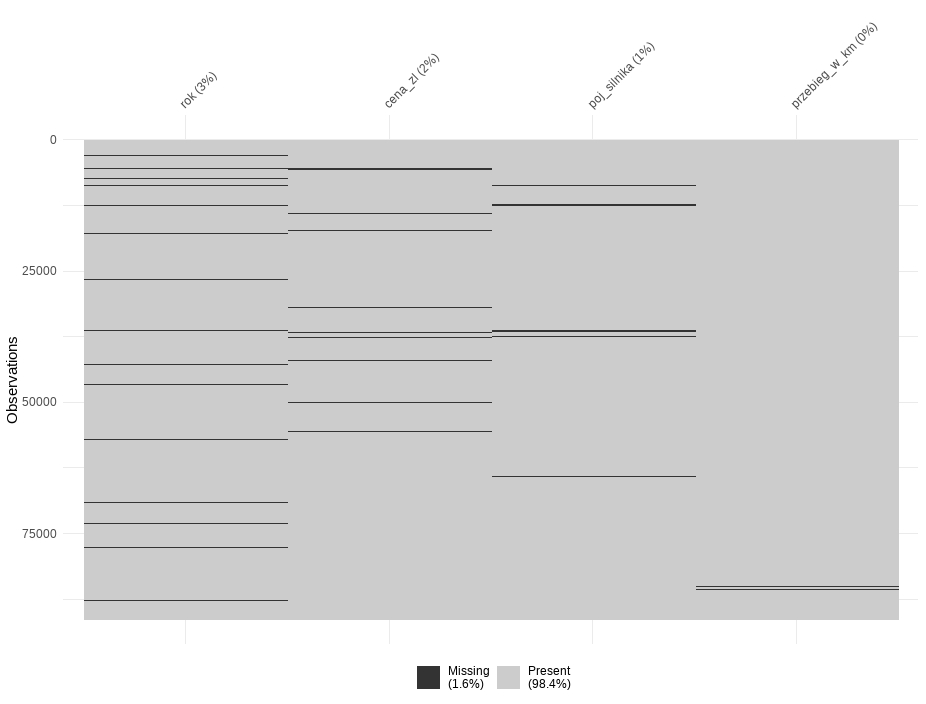
\includegraphics[width=1\linewidth]{images/1}

\begin{Shaded}
\begin{Highlighting}[]
\CommentTok{\# współwystępowanie NA między zmiennymi}
\FunctionTok{gg\_miss\_upset}\NormalTok{(dane[, }\FunctionTok{c}\NormalTok{(}\StringTok{"rok"}\NormalTok{, }\StringTok{"cena\_zl"}\NormalTok{, }\StringTok{"poj\_silnika"}\NormalTok{, }\StringTok{"przebieg\_w\_km"}\NormalTok{)], }
              \AttributeTok{nsets =} \DecValTok{4}\NormalTok{)}
\end{Highlighting}
\end{Shaded}

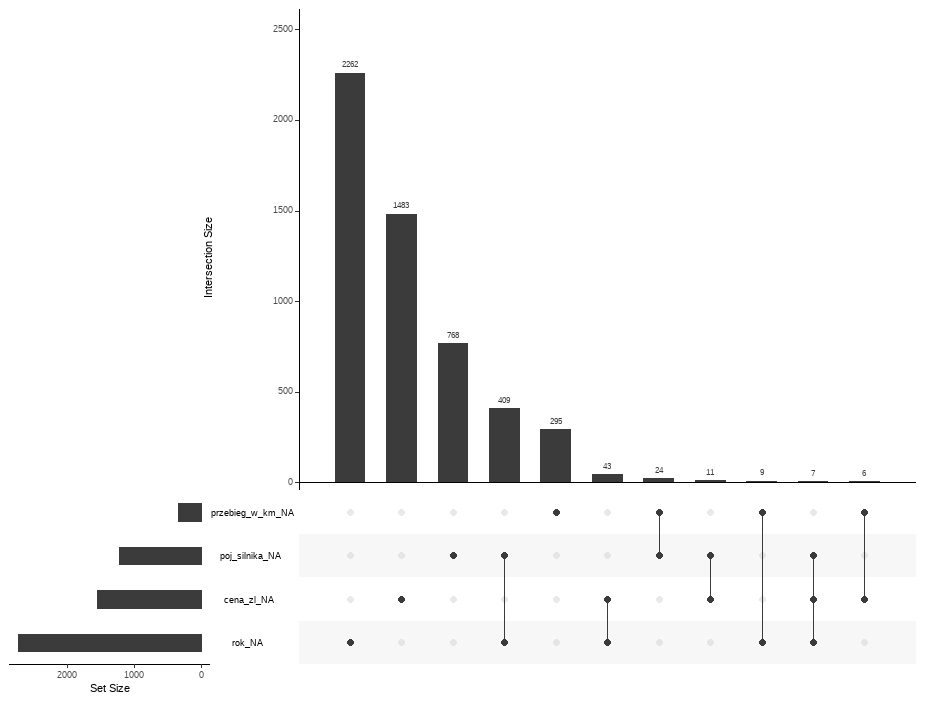
\includegraphics[width=1\linewidth]{images/2}

\begin{Shaded}
\begin{Highlighting}[]
\CommentTok{\# zależność występowania NA miedzy zmiennymi dotyczących ceny a rokiem }
\FunctionTok{ggplot}\NormalTok{(}\AttributeTok{data =}\NormalTok{ dane, }\FunctionTok{aes}\NormalTok{(}\AttributeTok{x =}\NormalTok{ rok, }\AttributeTok{y =}\NormalTok{ cena\_zl)) }\SpecialCharTok{+} 
  \FunctionTok{geom\_point}\NormalTok{() }\SpecialCharTok{+}
  \FunctionTok{geom\_miss\_point}\NormalTok{() }\SpecialCharTok{+}
  \FunctionTok{scale\_color\_manual}\NormalTok{(}\AttributeTok{values =} \FunctionTok{c}\NormalTok{(}\StringTok{"red"}\NormalTok{,}\StringTok{"navyblue"}\NormalTok{)) }\SpecialCharTok{+}
  \FunctionTok{theme\_minimal}\NormalTok{()}
\end{Highlighting}
\end{Shaded}

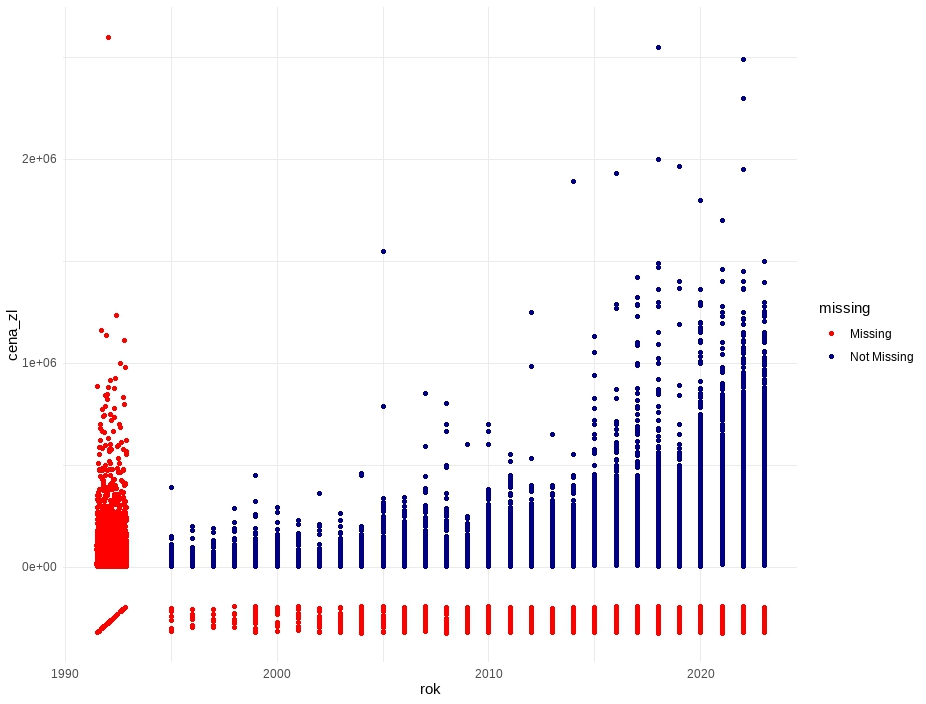
\includegraphics[width=1\linewidth]{images/3}

\begin{Shaded}
\begin{Highlighting}[]
\CommentTok{\# zależność występowania NA miedzy zmiennymi dotyczących roku a pojemności silnika }
\FunctionTok{ggplot}\NormalTok{(}\AttributeTok{data =}\NormalTok{ dane, }\FunctionTok{aes}\NormalTok{(}\AttributeTok{x =}\NormalTok{ rok, }\AttributeTok{y =}\NormalTok{ poj\_silnika)) }\SpecialCharTok{+} 
  \FunctionTok{geom\_point}\NormalTok{() }\SpecialCharTok{+}
  \FunctionTok{geom\_miss\_point}\NormalTok{() }\SpecialCharTok{+}
  \FunctionTok{scale\_color\_manual}\NormalTok{(}\AttributeTok{values =} \FunctionTok{c}\NormalTok{(}\StringTok{"orange"}\NormalTok{,}\StringTok{"green3"}\NormalTok{)) }\SpecialCharTok{+}
  \FunctionTok{theme\_minimal}\NormalTok{()}
\end{Highlighting}
\end{Shaded}

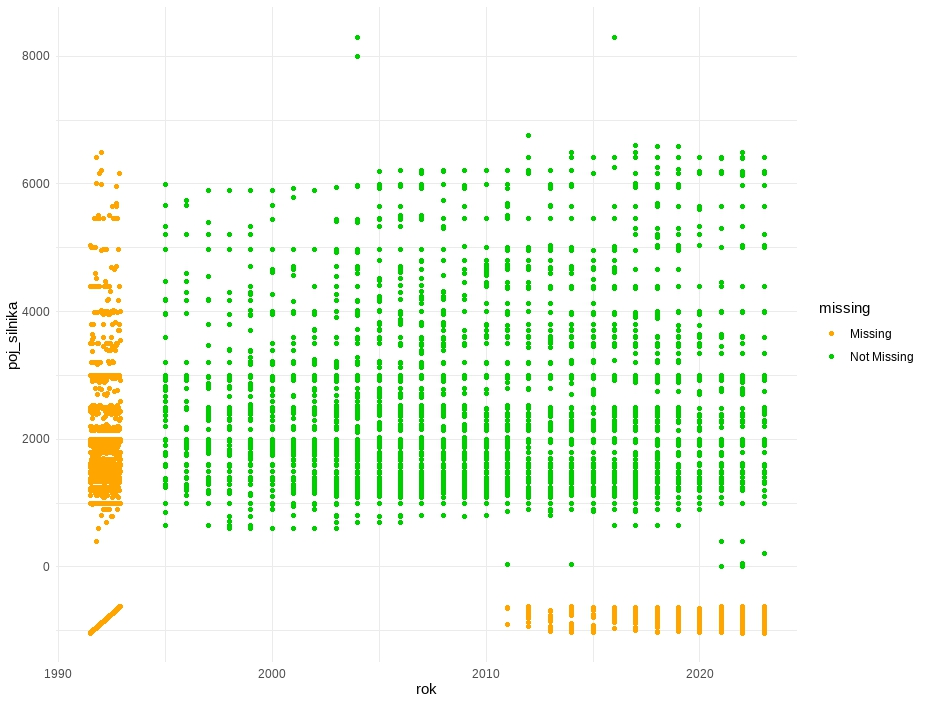
\includegraphics[width=1\linewidth]{images/4}

\begin{Shaded}
\begin{Highlighting}[]
\CommentTok{\# zależność występowania NA miedzy zmiennymi dotyczących roku a przebiegiem }
\FunctionTok{ggplot}\NormalTok{(}\AttributeTok{data =}\NormalTok{ dane, }\FunctionTok{aes}\NormalTok{(}\AttributeTok{x =}\NormalTok{ rok, }\AttributeTok{y =}\NormalTok{ przebieg\_w\_km)) }\SpecialCharTok{+} 
  \FunctionTok{geom\_point}\NormalTok{() }\SpecialCharTok{+}
  \FunctionTok{geom\_miss\_point}\NormalTok{() }\SpecialCharTok{+}
  \FunctionTok{scale\_color\_manual}\NormalTok{(}\AttributeTok{values =} \FunctionTok{c}\NormalTok{(}\StringTok{"gold"}\NormalTok{,}\StringTok{"steelblue1"}\NormalTok{)) }\SpecialCharTok{+}
  \FunctionTok{theme\_minimal}\NormalTok{()}
\end{Highlighting}
\end{Shaded}

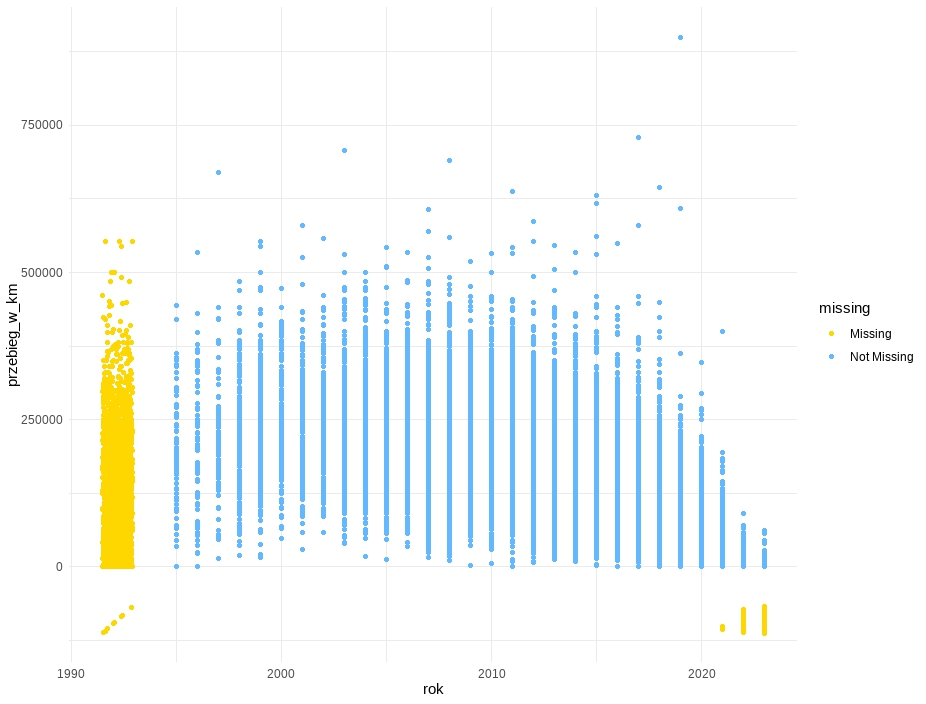
\includegraphics[width=1\linewidth]{images/5}

\begin{Shaded}
\begin{Highlighting}[]
\CommentTok{\# zależność występowania NA miedzy zmiennymi dotyczących pojemności silnika a ceną }
\FunctionTok{ggplot}\NormalTok{(}\AttributeTok{data =}\NormalTok{ dane, }\FunctionTok{aes}\NormalTok{(}\AttributeTok{x =}\NormalTok{ poj\_silnika, }\AttributeTok{y =}\NormalTok{ cena\_zl)) }\SpecialCharTok{+} 
  \FunctionTok{geom\_point}\NormalTok{() }\SpecialCharTok{+}
  \FunctionTok{geom\_miss\_point}\NormalTok{() }\SpecialCharTok{+}
  \FunctionTok{scale\_color\_manual}\NormalTok{(}\AttributeTok{values =} \FunctionTok{c}\NormalTok{(}\StringTok{"lightslateblue"}\NormalTok{,}\StringTok{"sienna1"}\NormalTok{)) }\SpecialCharTok{+}
  \FunctionTok{theme\_minimal}\NormalTok{()}
\end{Highlighting}
\end{Shaded}

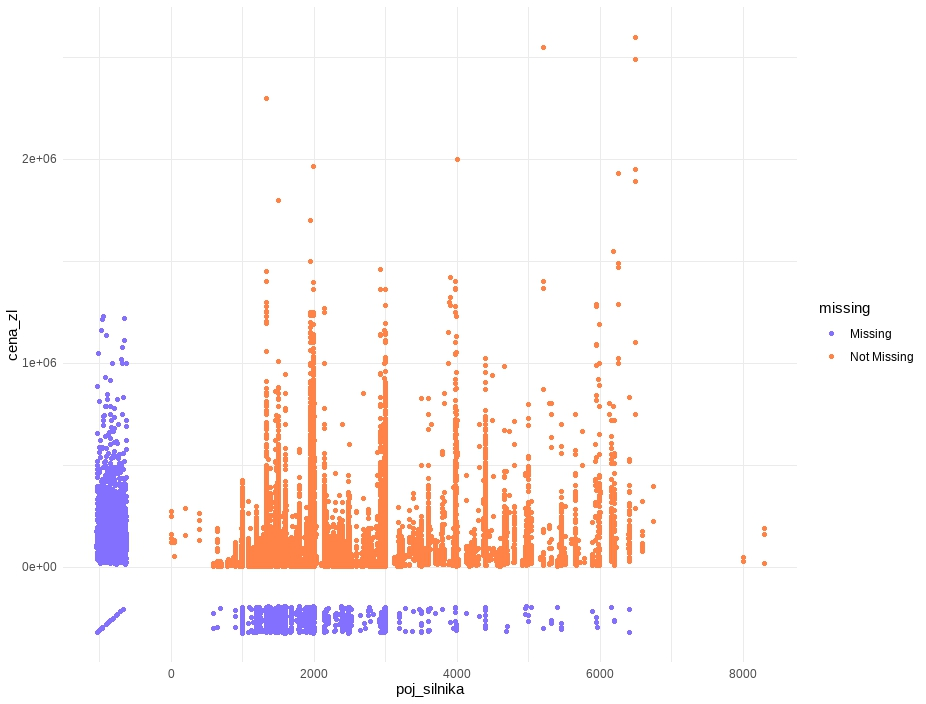
\includegraphics[width=1\linewidth]{images/6}

\begin{Shaded}
\begin{Highlighting}[]
\CommentTok{\# zależność występowania NA miedzy zmiennymi dotyczących ceny a przebiegu }
\FunctionTok{ggplot}\NormalTok{(}\AttributeTok{data =}\NormalTok{ dane, }\FunctionTok{aes}\NormalTok{(}\AttributeTok{x =}\NormalTok{ cena\_zl, }\AttributeTok{y =}\NormalTok{ przebieg\_w\_km)) }\SpecialCharTok{+} 
  \FunctionTok{geom\_point}\NormalTok{() }\SpecialCharTok{+}
  \FunctionTok{geom\_miss\_point}\NormalTok{() }\SpecialCharTok{+}
  \FunctionTok{scale\_color\_manual}\NormalTok{(}\AttributeTok{values =} \FunctionTok{c}\NormalTok{(}\StringTok{"magenta4"}\NormalTok{,}\StringTok{"turquoise4"}\NormalTok{)) }\SpecialCharTok{+}
  \FunctionTok{theme\_minimal}\NormalTok{()}
\end{Highlighting}
\end{Shaded}

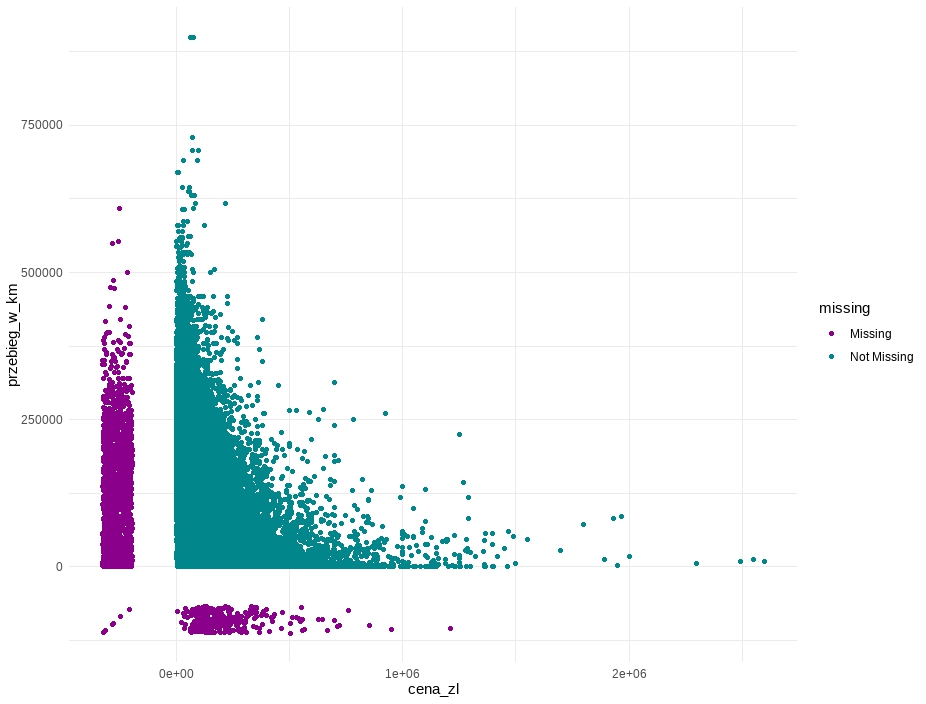
\includegraphics[width=1\linewidth]{images/7}

\begin{Shaded}
\begin{Highlighting}[]
\CommentTok{\# zależność występowania NA miedzy zmiennymi dotyczących pojemności silnika a przebiegiem }
\FunctionTok{ggplot}\NormalTok{(}\AttributeTok{data =}\NormalTok{ dane, }\FunctionTok{aes}\NormalTok{(}\AttributeTok{x =}\NormalTok{ poj\_silnika, }\AttributeTok{y =}\NormalTok{ przebieg\_w\_km)) }\SpecialCharTok{+} 
  \FunctionTok{geom\_point}\NormalTok{() }\SpecialCharTok{+}
  \FunctionTok{geom\_miss\_point}\NormalTok{() }\SpecialCharTok{+}
  \FunctionTok{scale\_color\_manual}\NormalTok{(}\AttributeTok{values =} \FunctionTok{c}\NormalTok{(}\StringTok{"hotpink3"}\NormalTok{,}\StringTok{"forestgreen"}\NormalTok{)) }\SpecialCharTok{+}
  \FunctionTok{theme\_minimal}\NormalTok{()}
\end{Highlighting}
\end{Shaded}

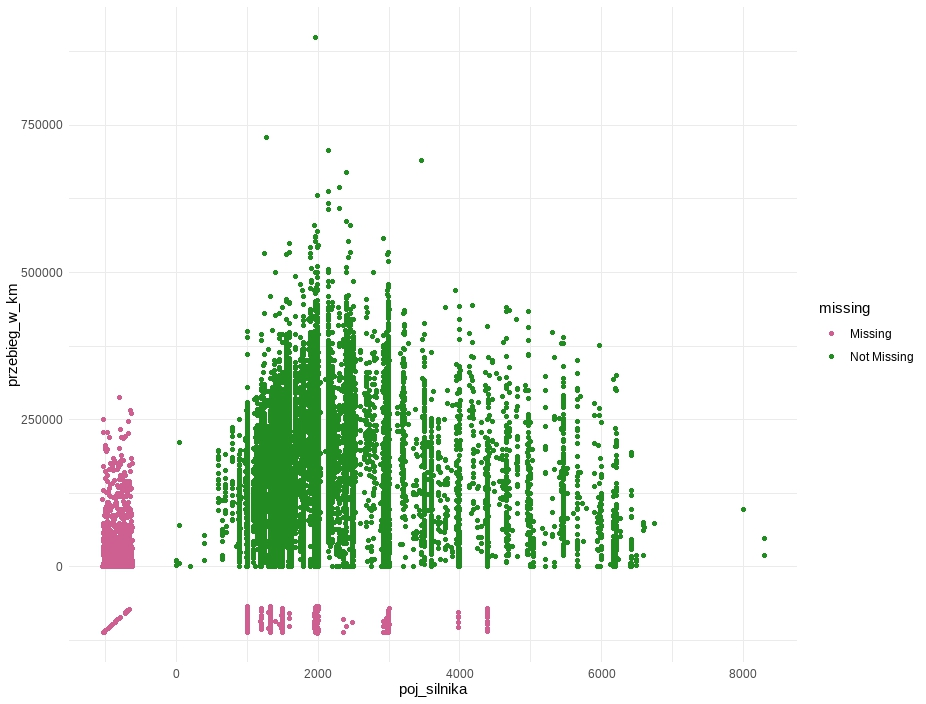
\includegraphics[width=1\linewidth]{images/8}

\begin{Shaded}
\begin{Highlighting}[]
\CommentTok{\# Procentowy udział brakujących wartości w podziale na typ paliwa}
\FunctionTok{gg\_miss\_var}\NormalTok{(dane, }\AttributeTok{facet =}\NormalTok{ paliwo, }\AttributeTok{show\_pct =} \ConstantTok{TRUE}\NormalTok{)}
\end{Highlighting}
\end{Shaded}

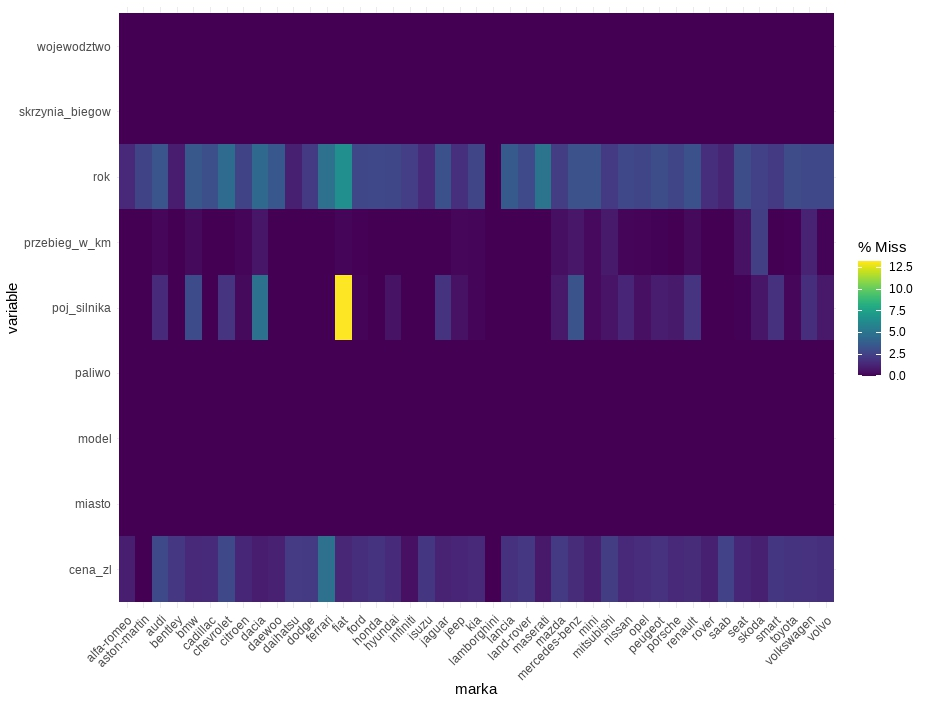
\includegraphics[width=1\linewidth]{images/9}

\begin{Shaded}
\begin{Highlighting}[]
\CommentTok{\# Heatmapa brakujących wartości z podziałem na markę}
\FunctionTok{gg\_miss\_fct}\NormalTok{(}\AttributeTok{x =}\NormalTok{ dane, }\AttributeTok{fct =}\NormalTok{ marka)}
\end{Highlighting}
\end{Shaded}

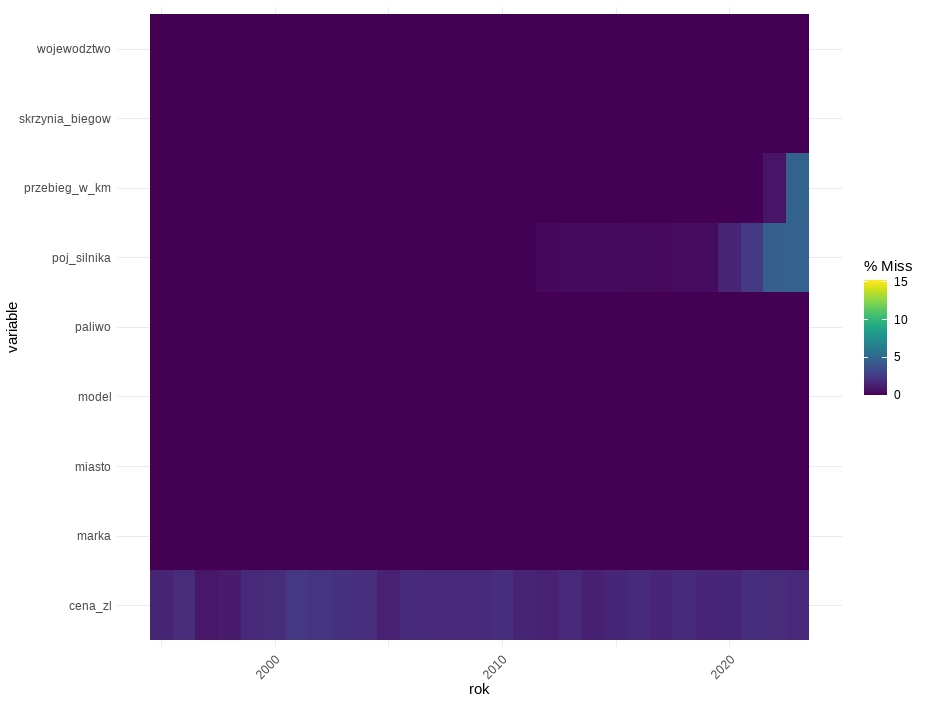
\includegraphics[width=1\linewidth]{images/10}

\begin{Shaded}
\begin{Highlighting}[]
\CommentTok{\# Heatmapa brakujących wartości z podziałem na rok}
\FunctionTok{gg\_miss\_fct}\NormalTok{(}\AttributeTok{x =}\NormalTok{ dane, }\AttributeTok{fct =}\NormalTok{ rok)}
\end{Highlighting}
\end{Shaded}

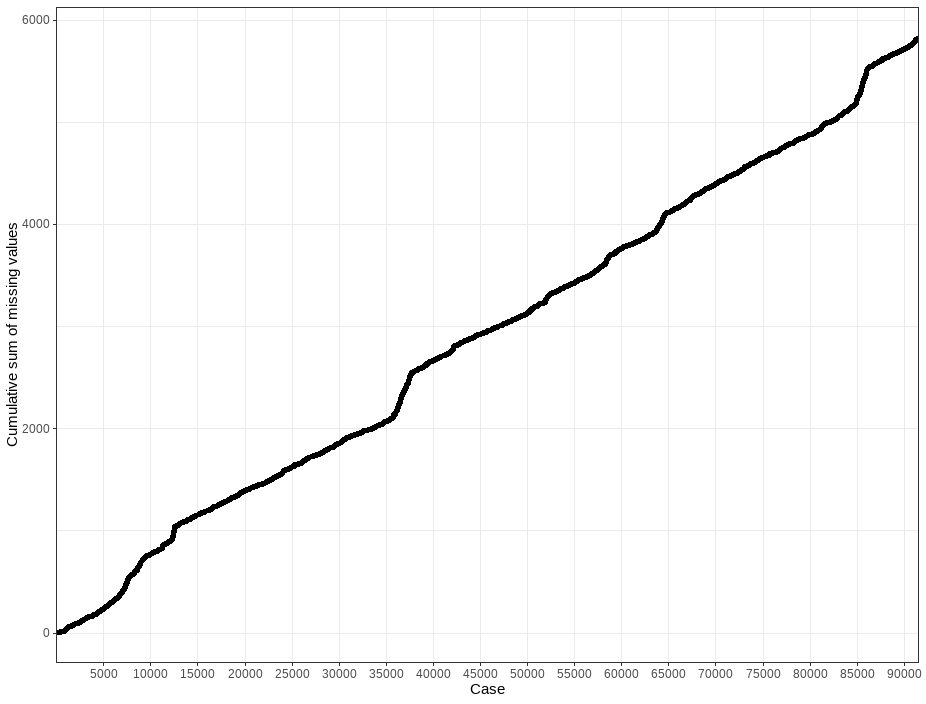
\includegraphics[width=1\linewidth]{images/11}

\begin{Shaded}
\begin{Highlighting}[]
\CommentTok{\# wykres skumulowana suma brakujących wartości}
\FunctionTok{gg\_miss\_case\_cumsum}\NormalTok{(dane, }\AttributeTok{breaks =} \DecValTok{5000}\NormalTok{) }\SpecialCharTok{+} \FunctionTok{theme\_bw}\NormalTok{()}
\end{Highlighting}
\end{Shaded}

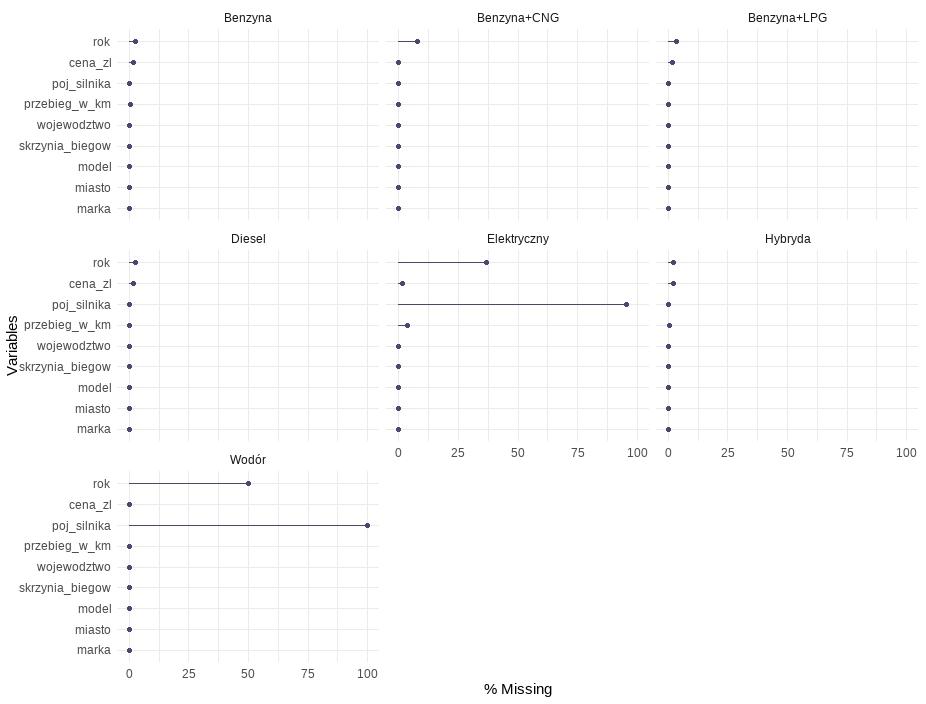
\includegraphics[width=1\linewidth]{images/12}

\subsubsection{Imputacje}\label{imputacje}

Dla wartości brakujących użyto imputacji KNN (K-Nearest Neighbors),
czyli metody najbliższych sąsiadów bazującej na zbliżonych wartościach
obserwacji. Użyto tej metody, ponieważ uwzględnia zależność miedzy
cechami. Istnieje duże prawdopodobieństwo, że te same modele samochodów
wyprodukowane w tych samych latach, będą miały zbliżony przebieg albo
wielkość silnika czy rodzaj paliwa. W przeciwieństwi do imputacji
średnią czy medianą, KNN dostosowuje się do struktury danych i nie
spłaszcza zmienności. Ze względu na duże podobieństwo między danymi
uznaliśmy tą metodę za najlepszą.

\begin{Shaded}
\begin{Highlighting}[]
\CommentTok{\# imputacja metodą KNN {-} metoda K{-}najbliższych sąsiadów}
\NormalTok{dane2 }\OtherTok{\textless{}{-}}\NormalTok{ dane}
\NormalTok{dane2\_knn }\OtherTok{\textless{}{-}} \FunctionTok{kNN}\NormalTok{(dane2)}
\NormalTok{daneknn }\OtherTok{\textless{}{-}}\NormalTok{ dane2\_knn }\SpecialCharTok{\%\textgreater{}\%} \FunctionTok{select}\NormalTok{(}\FunctionTok{where}\NormalTok{(}\SpecialCharTok{\textasciitilde{}} \SpecialCharTok{!}\FunctionTok{is.logical}\NormalTok{(.)))}
\FunctionTok{n\_miss}\NormalTok{(daneknn)}
\end{Highlighting}
\end{Shaded}

\subsubsection{Analiza opisowa}\label{analiza-opisowa}

W celu lepszego zrozumienia danych oraz ich potencjalnego wykorzystania
przeprowadziliśmy analizę opisową. Dla skutecznego wykorzystania danych,
usunęliśmy zbędne spacje z nazw kolumn, zapisaliśmy niektóre kolumny
jako wartości numeryczne oraz wybraliśmy biblioteki z których będziemy
korzystać dla przeprowadzenia testów statystycznych oraz wizualizacji
danych

\begin{Shaded}
\begin{Highlighting}[]
\CommentTok{\# Usunięcie zbędnych spacji z nazw kolumn}
\FunctionTok{colnames}\NormalTok{(dane) }\OtherTok{\textless{}{-}} \FunctionTok{trimws}\NormalTok{(}\FunctionTok{colnames}\NormalTok{(dane))}

\CommentTok{\# Konwersja odpowiednich kolumn na wartości numeryczne}
\NormalTok{dane}\SpecialCharTok{$}\NormalTok{poj\_silnika }\OtherTok{\textless{}{-}} \FunctionTok{as.numeric}\NormalTok{(}\FunctionTok{gsub}\NormalTok{(}\StringTok{"[\^{}0{-}9]"}\NormalTok{, }\StringTok{""}\NormalTok{, dane}\SpecialCharTok{$}\NormalTok{poj\_silnika))}
\NormalTok{dane}\SpecialCharTok{$}\NormalTok{przebieg\_w\_km }\OtherTok{\textless{}{-}} \FunctionTok{as.numeric}\NormalTok{(}\FunctionTok{gsub}\NormalTok{(}\StringTok{"[\^{}0{-}9]"}\NormalTok{, }\StringTok{""}\NormalTok{, dane}\SpecialCharTok{$}\NormalTok{przebieg\_w\_km))}
\NormalTok{dane}\SpecialCharTok{$}\NormalTok{rok }\OtherTok{\textless{}{-}} \FunctionTok{as.numeric}\NormalTok{(dane}\SpecialCharTok{$}\NormalTok{rok)}

\CommentTok{\# Ładowanie bibliotek}
\FunctionTok{library}\NormalTok{(dplyr)}
\FunctionTok{library}\NormalTok{(ggplot2)}
\FunctionTok{library}\NormalTok{(ggstatsplot)}
\FunctionTok{library}\NormalTok{(corrplot)}
\FunctionTok{library}\NormalTok{(knitr)}
\end{Highlighting}
\end{Shaded}

Pierwszym krokiem naszej analizie jest przedstawienie danych jako tabel
liczności

\begin{Shaded}
\begin{Highlighting}[]
\CommentTok{\# 1. Tabele liczności dla każdej zmiennej}
\NormalTok{tabele }\OtherTok{\textless{}{-}} \FunctionTok{list}\NormalTok{(}
  \AttributeTok{marka =}\NormalTok{ dane }\SpecialCharTok{\%\textgreater{}\%} \FunctionTok{count}\NormalTok{(marka, }\AttributeTok{sort =} \ConstantTok{TRUE}\NormalTok{),}
  \AttributeTok{model =}\NormalTok{ dane }\SpecialCharTok{\%\textgreater{}\%} \FunctionTok{count}\NormalTok{(model, }\AttributeTok{sort =} \ConstantTok{TRUE}\NormalTok{),}
  \AttributeTok{wojewodztwo =}\NormalTok{ dane }\SpecialCharTok{\%\textgreater{}\%} \FunctionTok{count}\NormalTok{(wojewodztwo, }\AttributeTok{sort =} \ConstantTok{TRUE}\NormalTok{),}
  \AttributeTok{rok =}\NormalTok{ dane }\SpecialCharTok{\%\textgreater{}\%} \FunctionTok{count}\NormalTok{(rok, }\AttributeTok{sort =} \ConstantTok{TRUE}\NormalTok{),}
  \AttributeTok{paliwo =}\NormalTok{ dane }\SpecialCharTok{\%\textgreater{}\%} \FunctionTok{count}\NormalTok{(paliwo, }\AttributeTok{sort =} \ConstantTok{TRUE}\NormalTok{),}
  \AttributeTok{skrzynia\_biegow =}\NormalTok{ dane }\SpecialCharTok{\%\textgreater{}\%} \FunctionTok{count}\NormalTok{(skrzynia\_biegow, }\AttributeTok{sort =} \ConstantTok{TRUE}\NormalTok{),}
  \AttributeTok{poj\_silnika =}\NormalTok{ dane }\SpecialCharTok{\%\textgreater{}\%} \FunctionTok{count}\NormalTok{(poj\_silnika, }\AttributeTok{sort =} \ConstantTok{TRUE}\NormalTok{),}
  \AttributeTok{miasto =}\NormalTok{  dane }\SpecialCharTok{\%\textgreater{}\%} \FunctionTok{count}\NormalTok{(miasto, }\AttributeTok{sort =} \ConstantTok{TRUE}\NormalTok{)}
\NormalTok{)}

\CommentTok{\# Wyświetlenie tabel liczności}
\NormalTok{tabele\_md }\OtherTok{\textless{}{-}} \FunctionTok{lapply}\NormalTok{(tabele, }\ControlFlowTok{function}\NormalTok{(tbl) \{}
  \FunctionTok{kable}\NormalTok{(tbl, }\AttributeTok{format =} \StringTok{"markdown"}\NormalTok{, }\AttributeTok{col.names =} \FunctionTok{c}\NormalTok{(}\StringTok{"Kategoria"}\NormalTok{, }\StringTok{"Liczba"}\NormalTok{))}
\NormalTok{\})}

\CommentTok{\# Wyświetlenie tabel}
\FunctionTok{names}\NormalTok{(tabele\_md) }\OtherTok{\textless{}{-}} \FunctionTok{c}\NormalTok{(}\StringTok{"Marka"}\NormalTok{, }\StringTok{"Model"}\NormalTok{, }\StringTok{"Województwo"}\NormalTok{, }\StringTok{"Rok"}\NormalTok{, }\StringTok{"Paliwo"}\NormalTok{, }\StringTok{"Skrzynia biegów"}\NormalTok{, }\StringTok{"Pojemność silnika"}\NormalTok{, }\StringTok{"Miasto"}\NormalTok{)}

\ControlFlowTok{for}\NormalTok{ (nazwa }\ControlFlowTok{in} \FunctionTok{names}\NormalTok{(tabele\_md)) \{}
  \FunctionTok{cat}\NormalTok{(}\FunctionTok{paste0}\NormalTok{(}\StringTok{"}\SpecialCharTok{\textbackslash{}n}\StringTok{\#\# "}\NormalTok{, nazwa, }\StringTok{"}\SpecialCharTok{\textbackslash{}n\textbackslash{}n}\StringTok{"}\NormalTok{)) }
  \FunctionTok{cat}\NormalTok{(tabele\_md[[nazwa]], }\StringTok{"}\SpecialCharTok{\textbackslash{}n\textbackslash{}n}\StringTok{"}\NormalTok{)   }
\NormalTok{\}}
\end{Highlighting}
\end{Shaded}

Na podstawie tabeli liczności, możemy zobaczyć między innymi ilość
transakcji w każdym mieście lub województwie, ile zostało
przeprowadzonych transakcji z samochodami o danych charakterystykach.

\begin{Shaded}
\begin{Highlighting}[]
\NormalTok{tabele }\OtherTok{\textless{}{-}} \FunctionTok{lapply}\NormalTok{(tabele, }\ControlFlowTok{function}\NormalTok{(tbl) \{}
  \FunctionTok{colnames}\NormalTok{(tbl) }\OtherTok{\textless{}{-}} \FunctionTok{c}\NormalTok{(}\StringTok{"Kategoria"}\NormalTok{, }\StringTok{"n"}\NormalTok{)}
\NormalTok{  tbl}
\NormalTok{\})}

\ControlFlowTok{for}\NormalTok{ (nazwa }\ControlFlowTok{in} \FunctionTok{names}\NormalTok{(tabele)) \{}
\NormalTok{  tabela }\OtherTok{\textless{}{-}}\NormalTok{ tabele[[nazwa]]}
  
  \CommentTok{\# Tworzenie wykresu}
\NormalTok{  p }\OtherTok{\textless{}{-}} \FunctionTok{ggplot}\NormalTok{(tabela, }\FunctionTok{aes}\NormalTok{(}\AttributeTok{x =} \FunctionTok{reorder}\NormalTok{(Kategoria, n), }\AttributeTok{y =}\NormalTok{ n)) }\SpecialCharTok{+}
    \FunctionTok{geom\_bar}\NormalTok{(}\AttributeTok{stat =} \StringTok{"identity"}\NormalTok{, }\AttributeTok{fill =} \StringTok{"steelblue"}\NormalTok{) }\SpecialCharTok{+}
    \FunctionTok{coord\_flip}\NormalTok{() }\SpecialCharTok{+}
    \FunctionTok{labs}\NormalTok{(}
      \AttributeTok{title =} \FunctionTok{paste}\NormalTok{(}\StringTok{"Liczba samochodów wg"}\NormalTok{, nazwa),}
      \AttributeTok{x =}\NormalTok{ nazwa,}
      \AttributeTok{y =} \StringTok{"Liczba"}
\NormalTok{    ) }\SpecialCharTok{+}
    \FunctionTok{theme\_minimal}\NormalTok{()}
  
  \CommentTok{\# Zapis wykresu}
  \FunctionTok{ggsave}\NormalTok{(}\FunctionTok{paste0}\NormalTok{(}\StringTok{"wykres\_"}\NormalTok{, nazwa, }\StringTok{".png"}\NormalTok{), }\AttributeTok{plot =}\NormalTok{ p, }\AttributeTok{width =} \DecValTok{8}\NormalTok{, }\AttributeTok{height =} \DecValTok{6}\NormalTok{)}
\NormalTok{\}}
\end{Highlighting}
\end{Shaded}

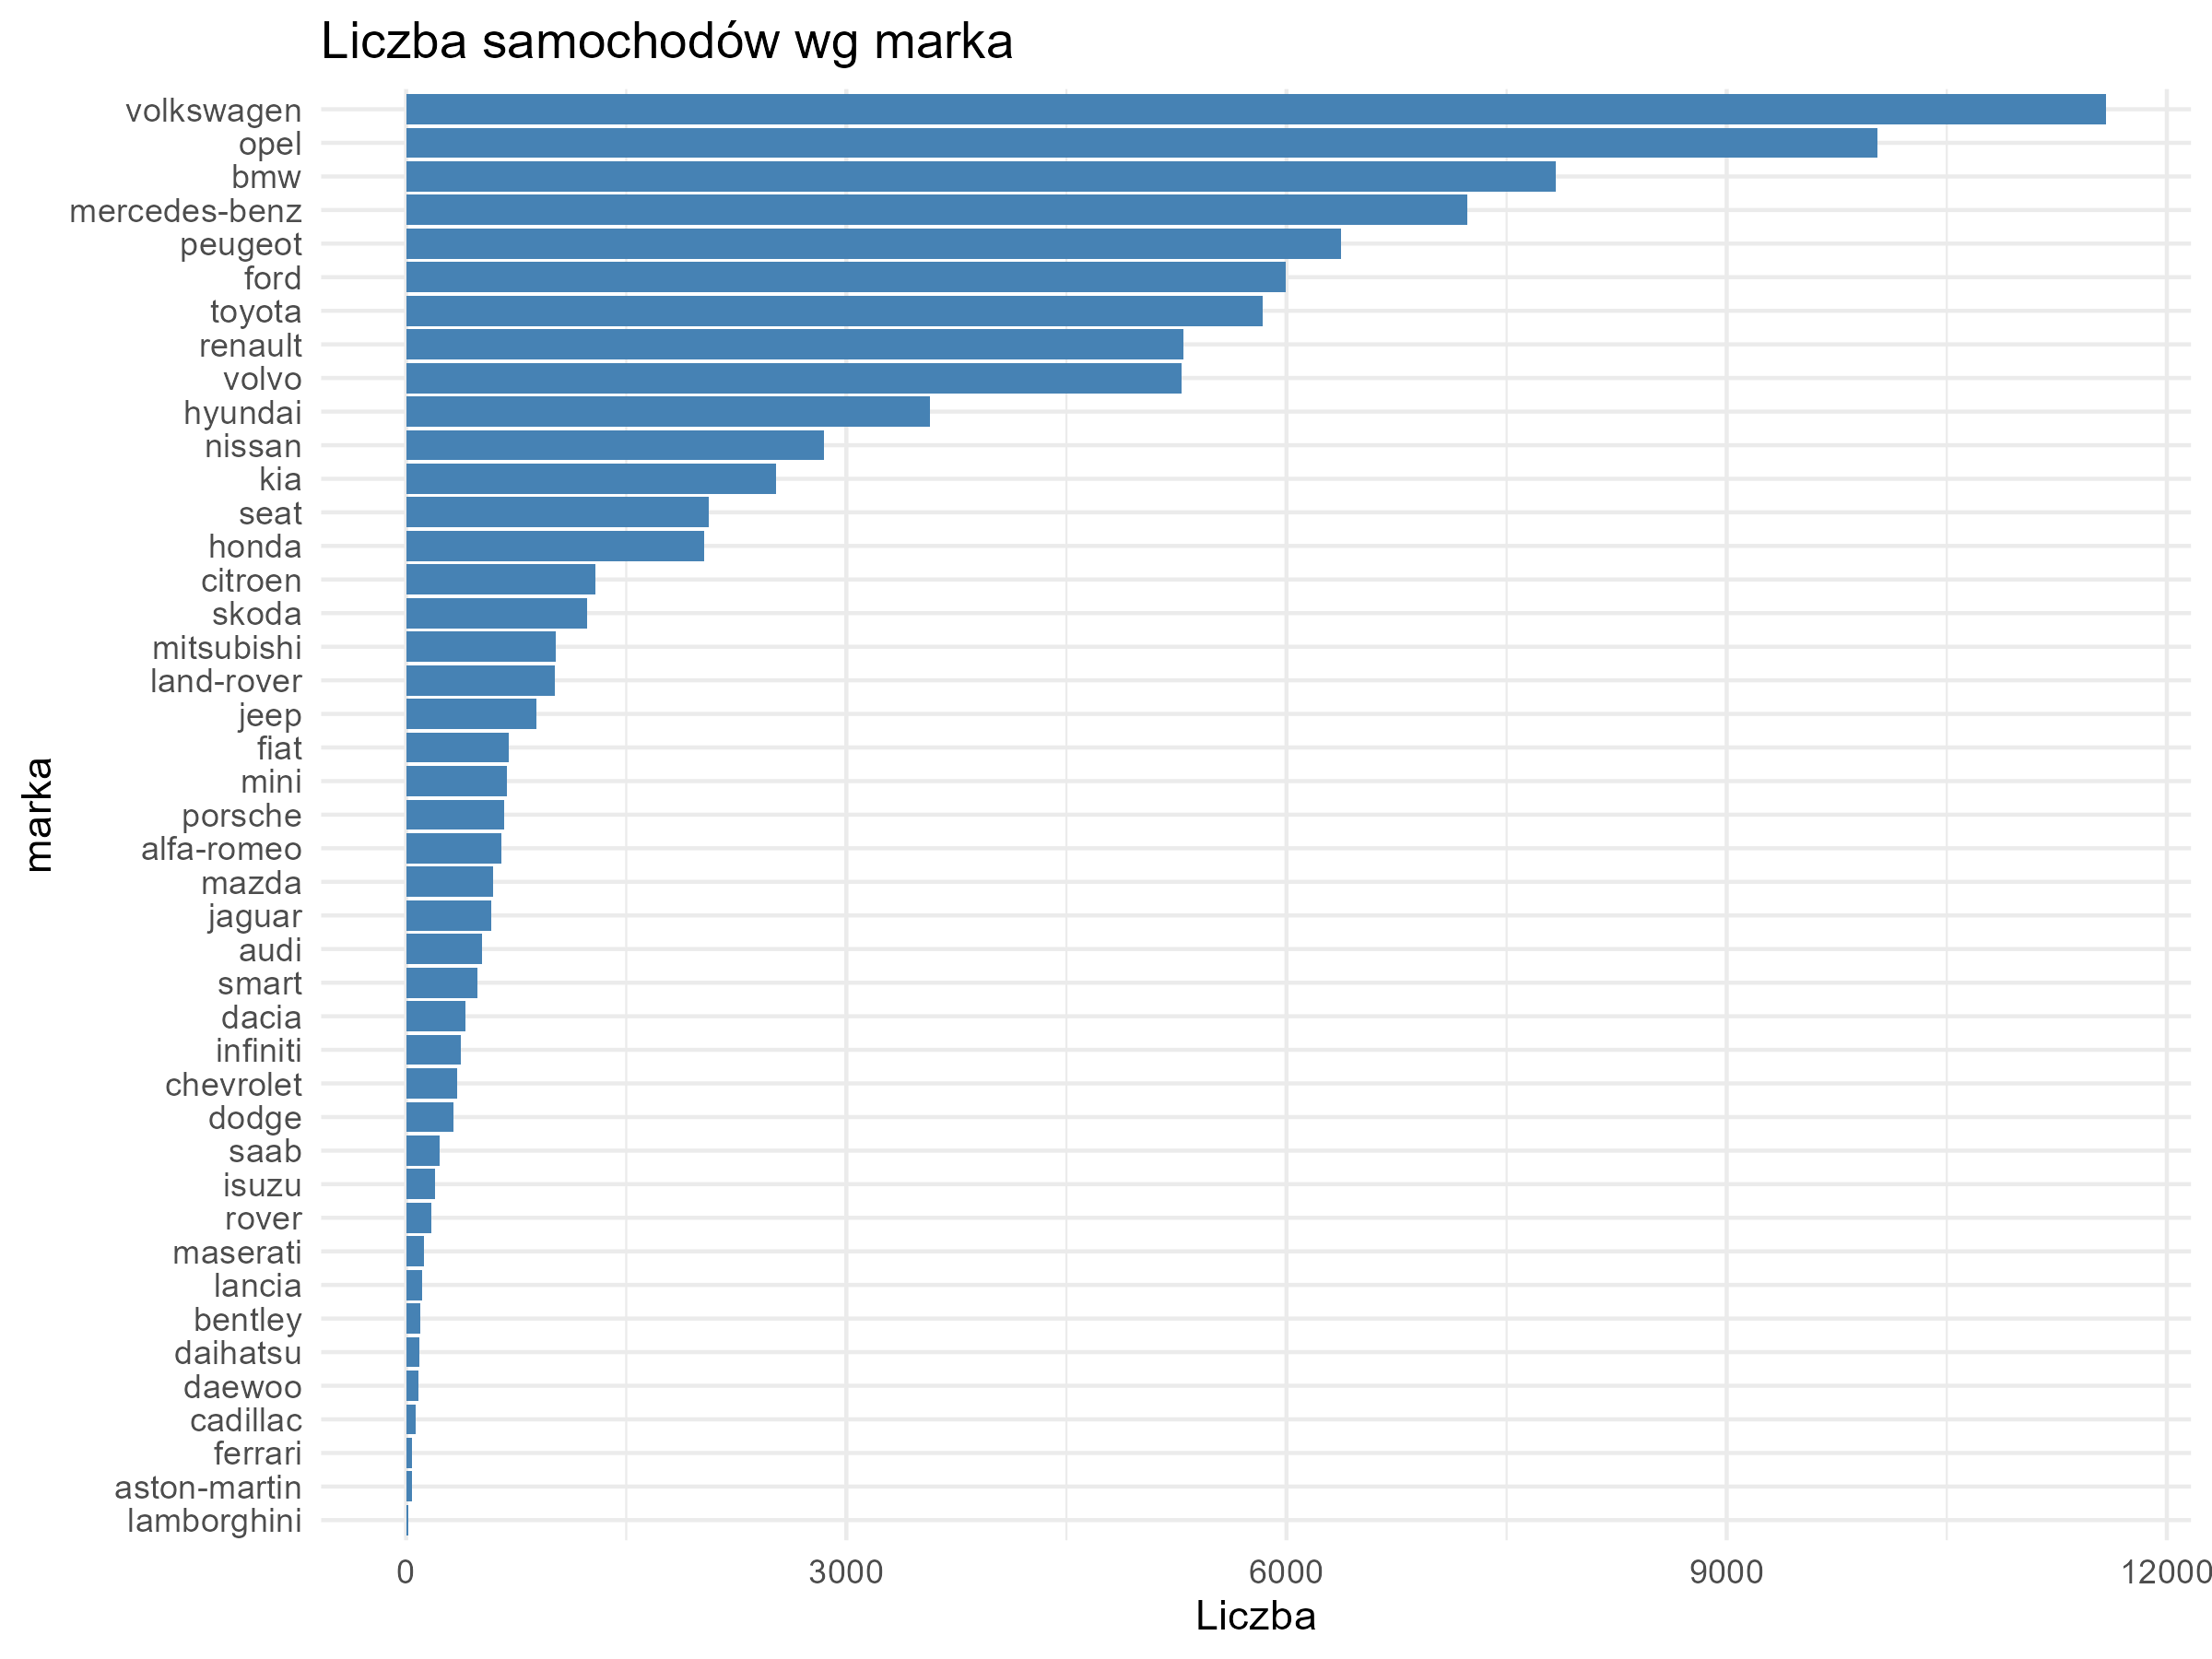
\includegraphics[width=1\linewidth]{analiza/wykres_marka}

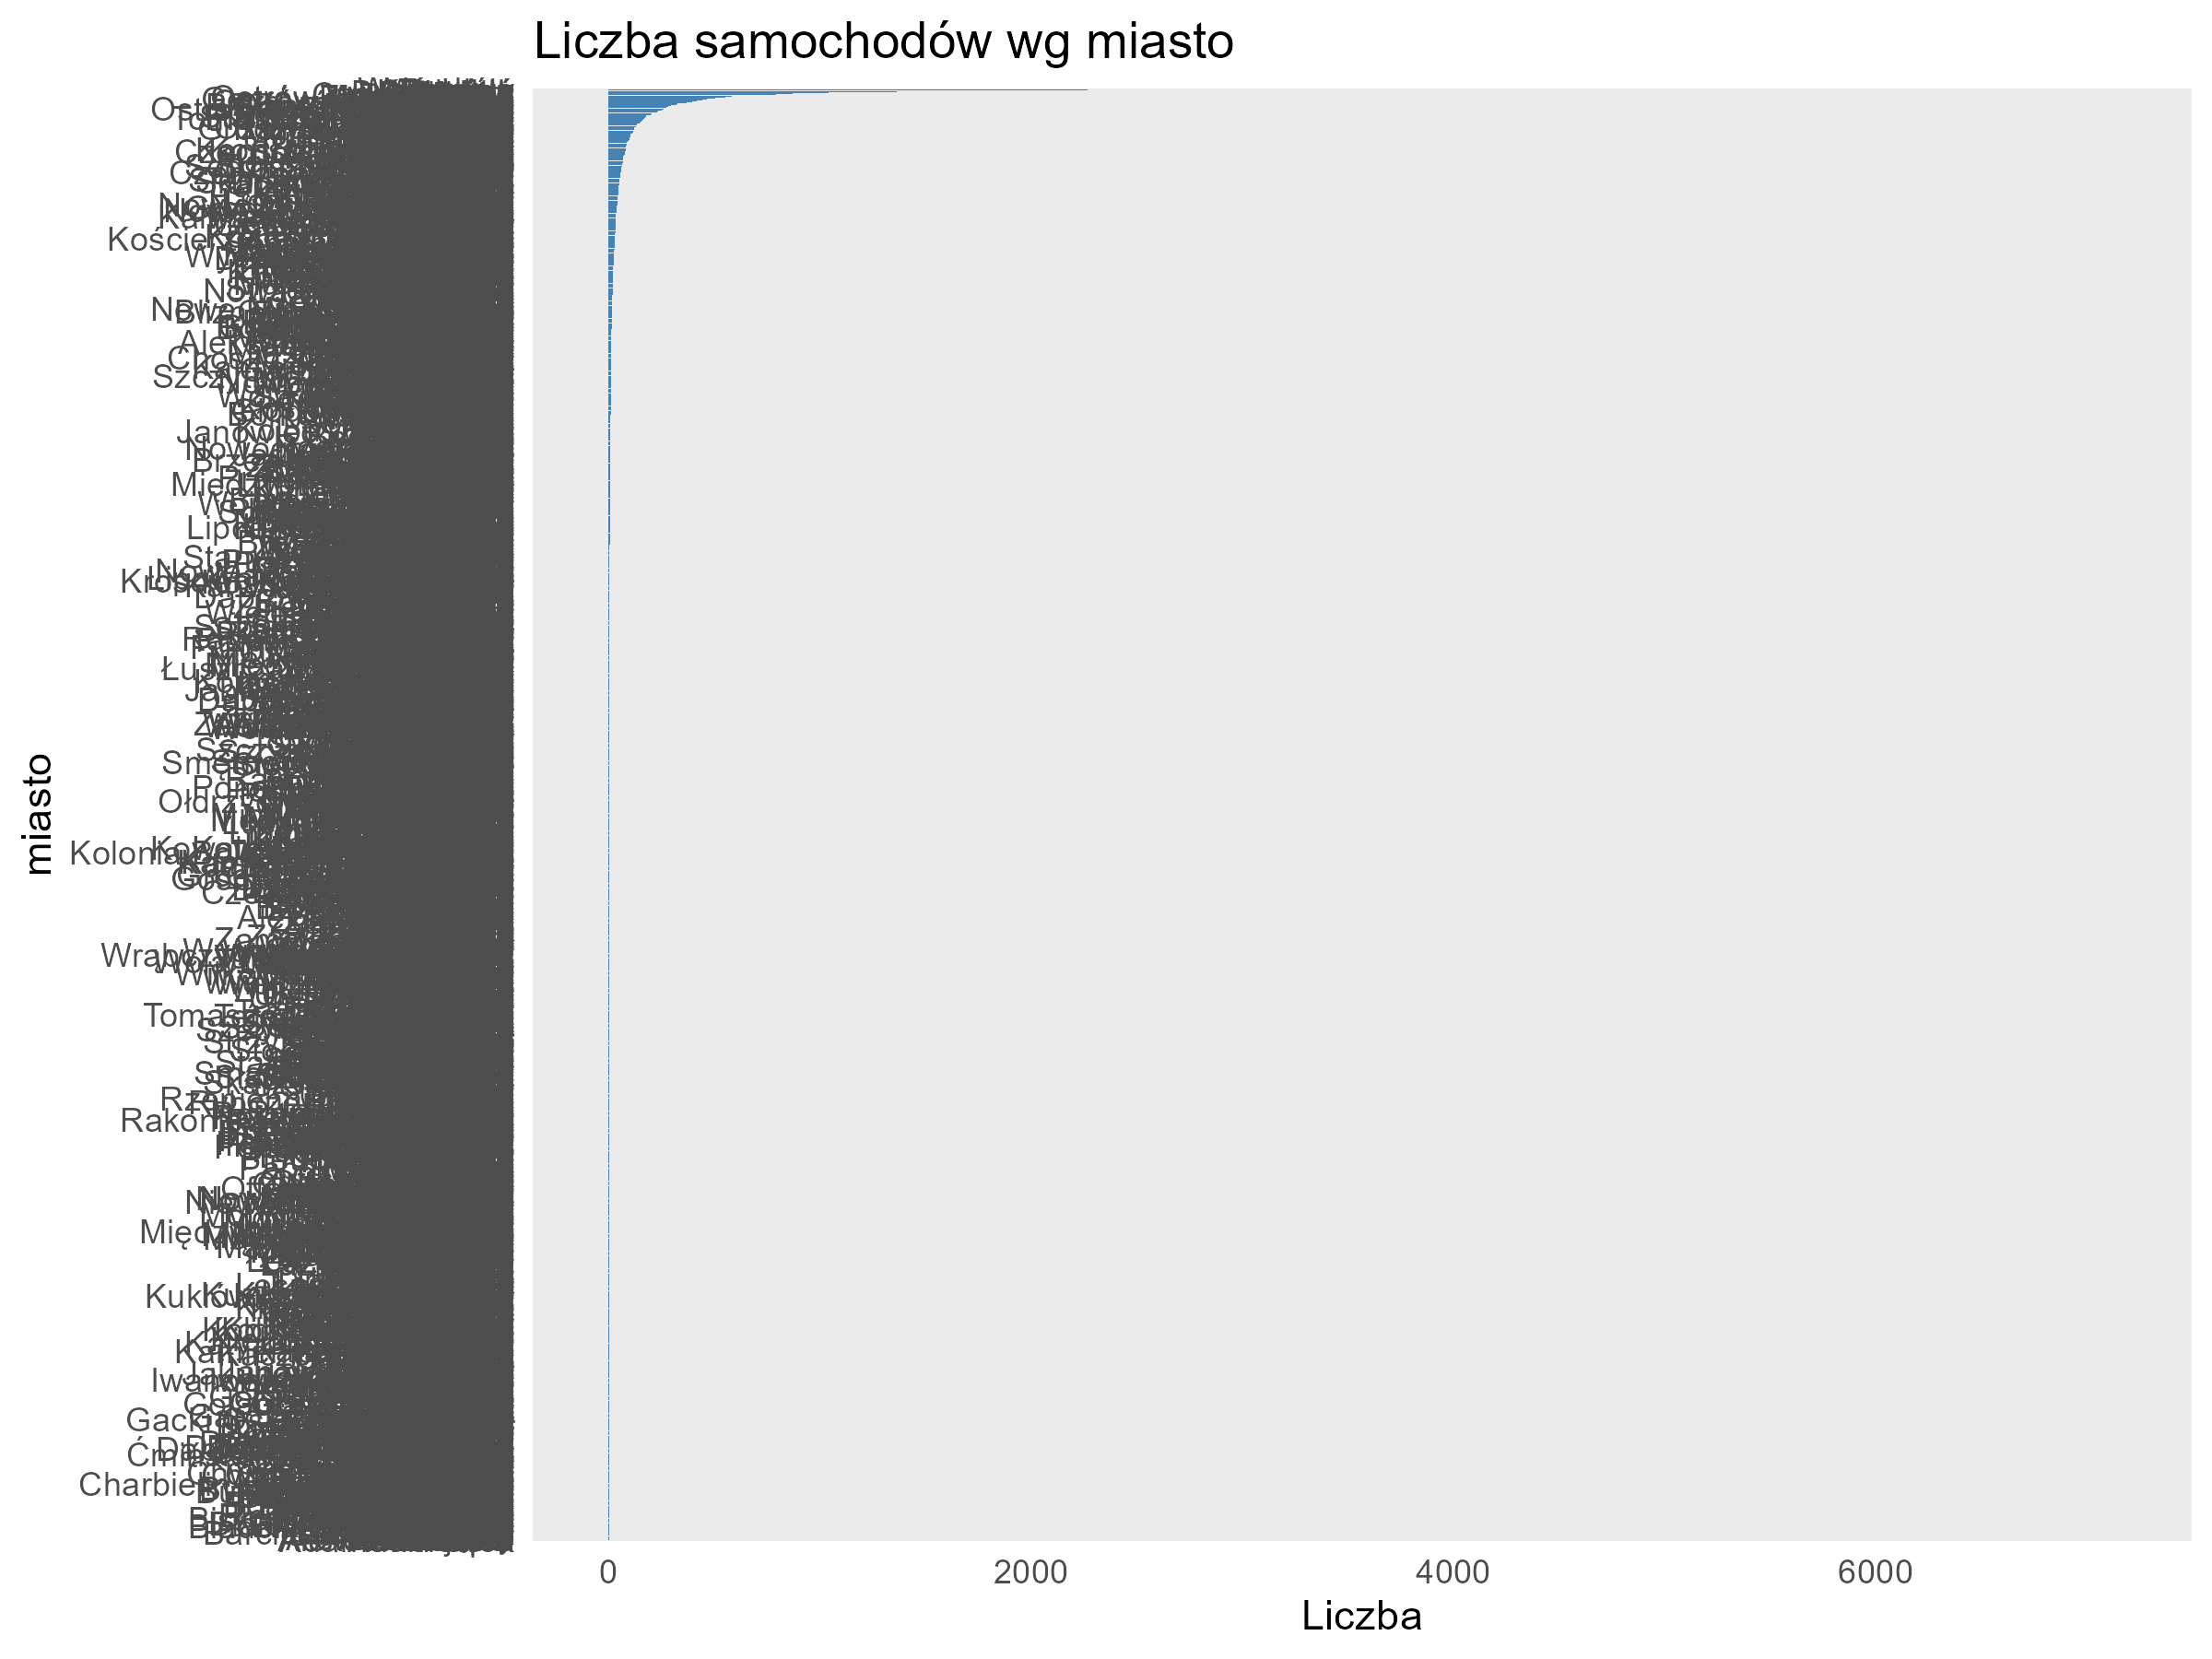
\includegraphics[width=1\linewidth]{analiza/wykres_miasto}

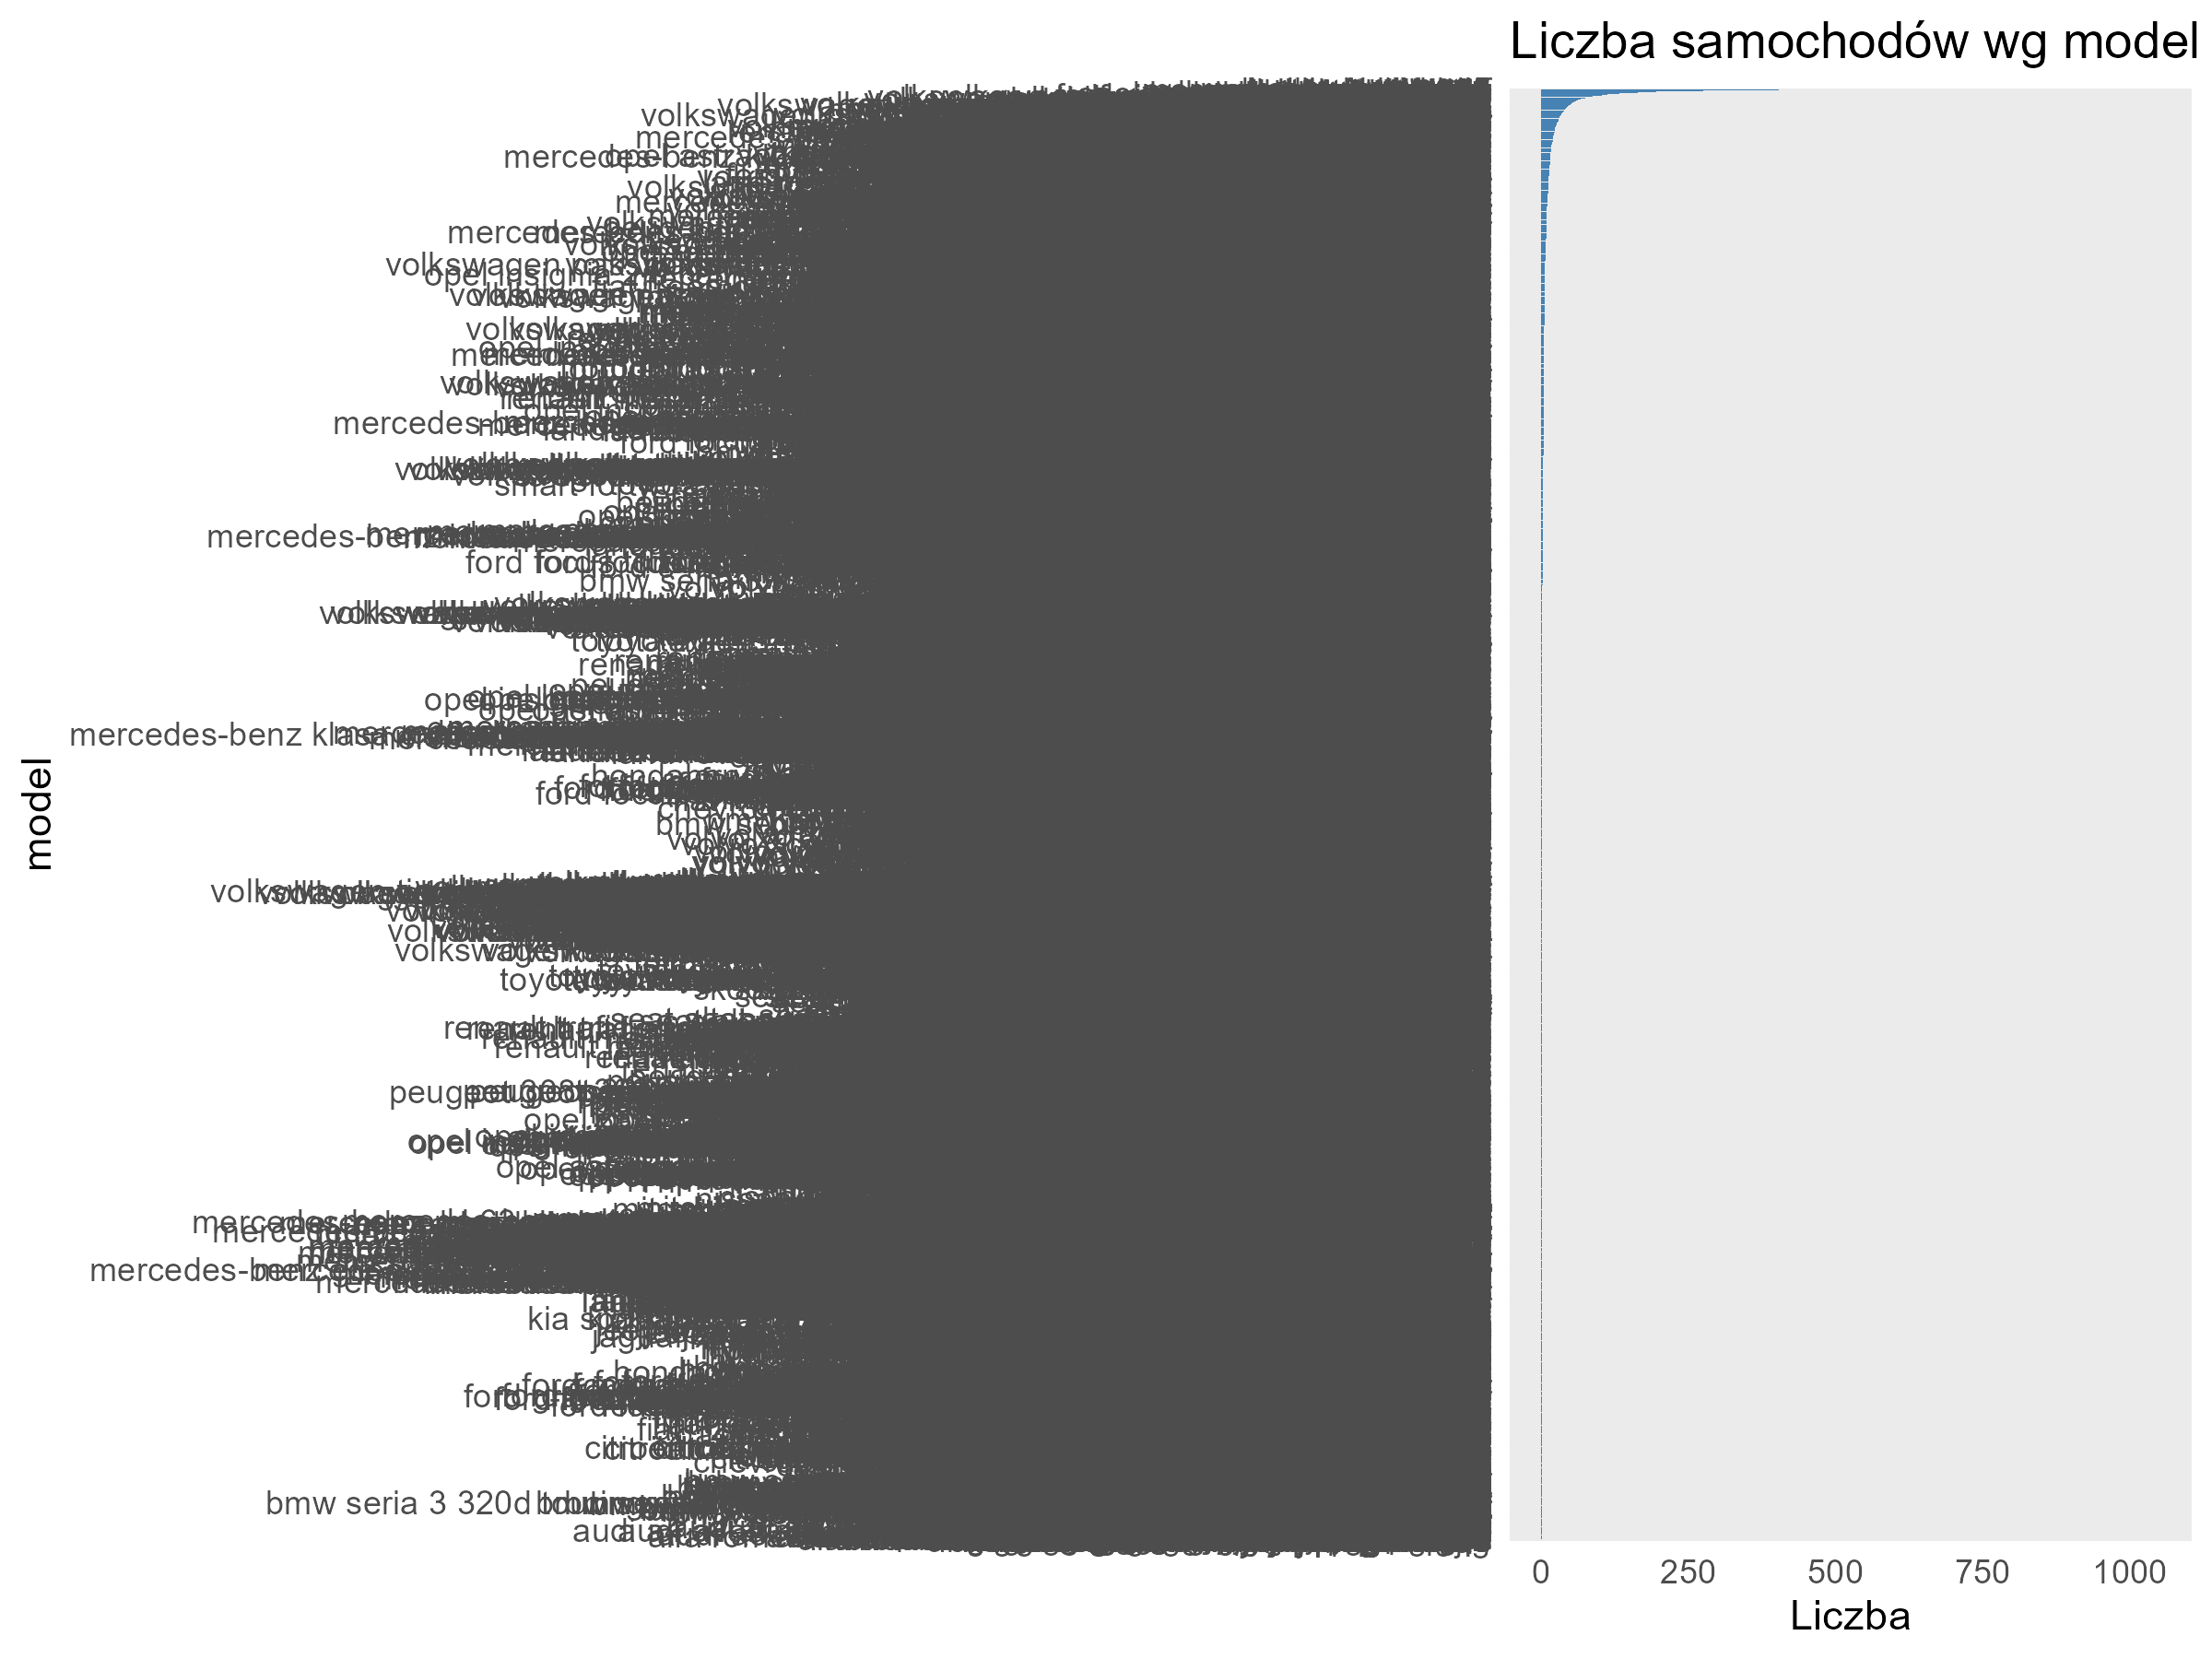
\includegraphics[width=1\linewidth]{analiza/wykres_model}

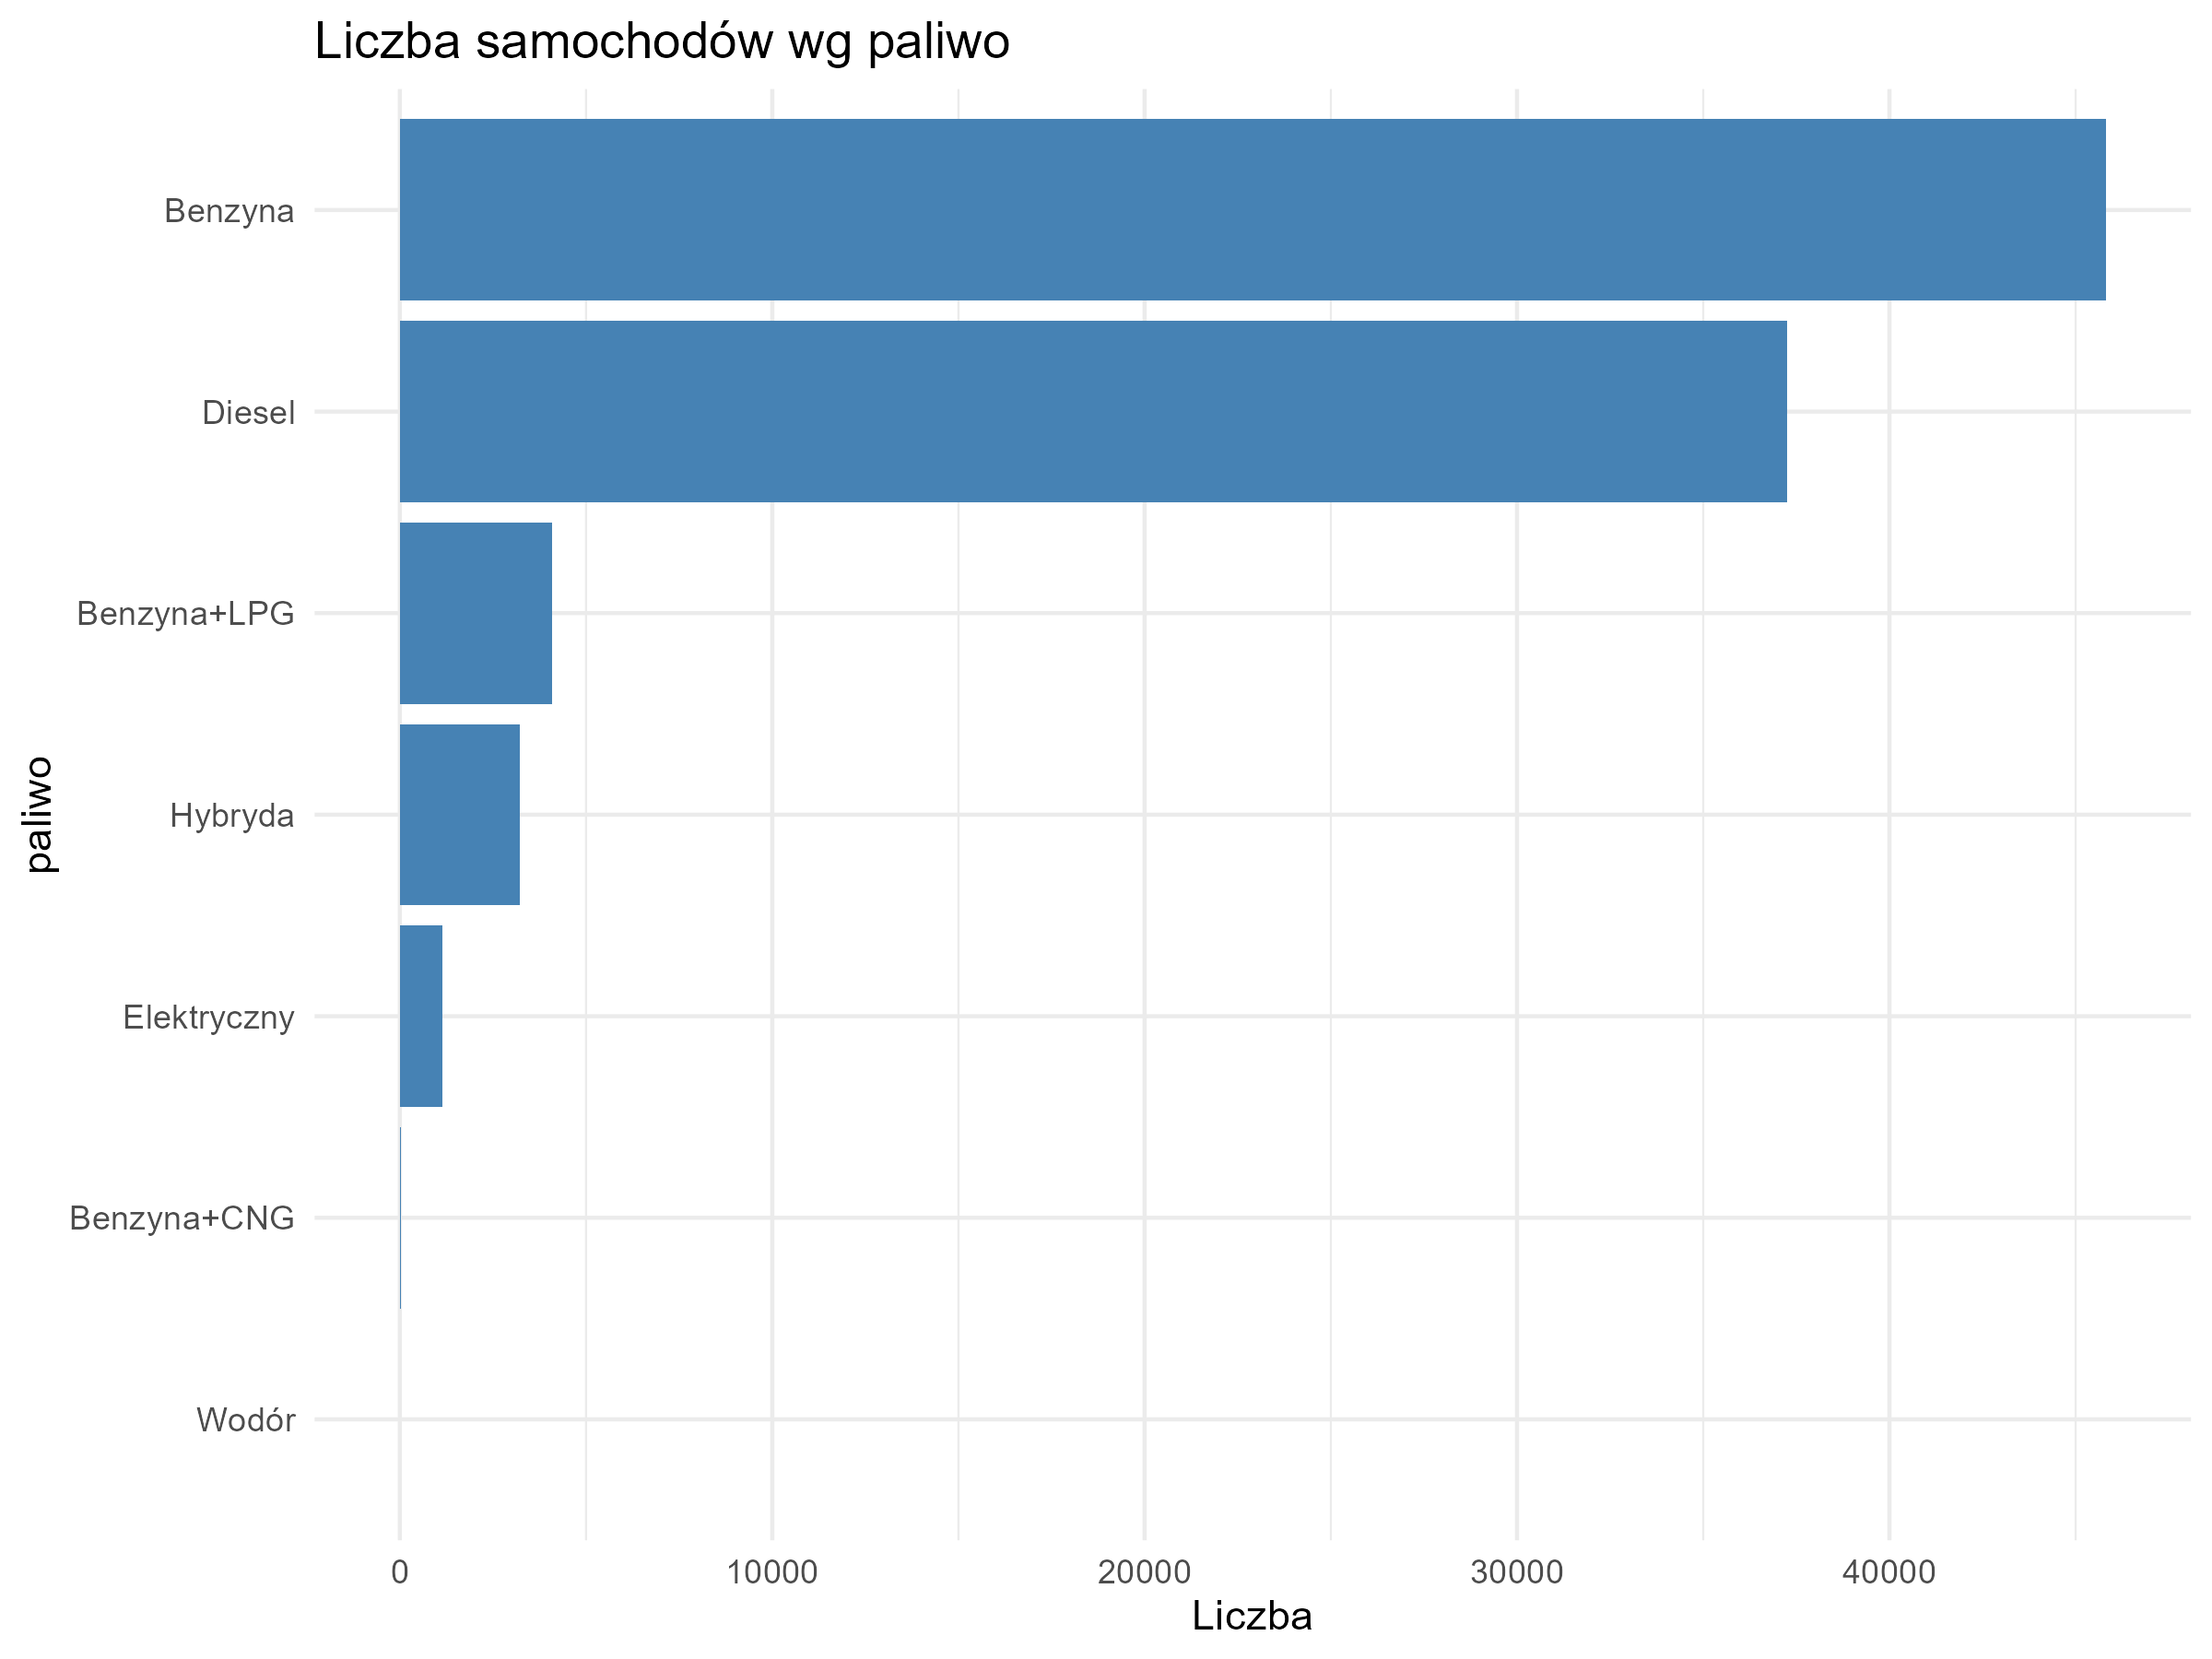
\includegraphics[width=1\linewidth]{analiza/wykres_paliwo}

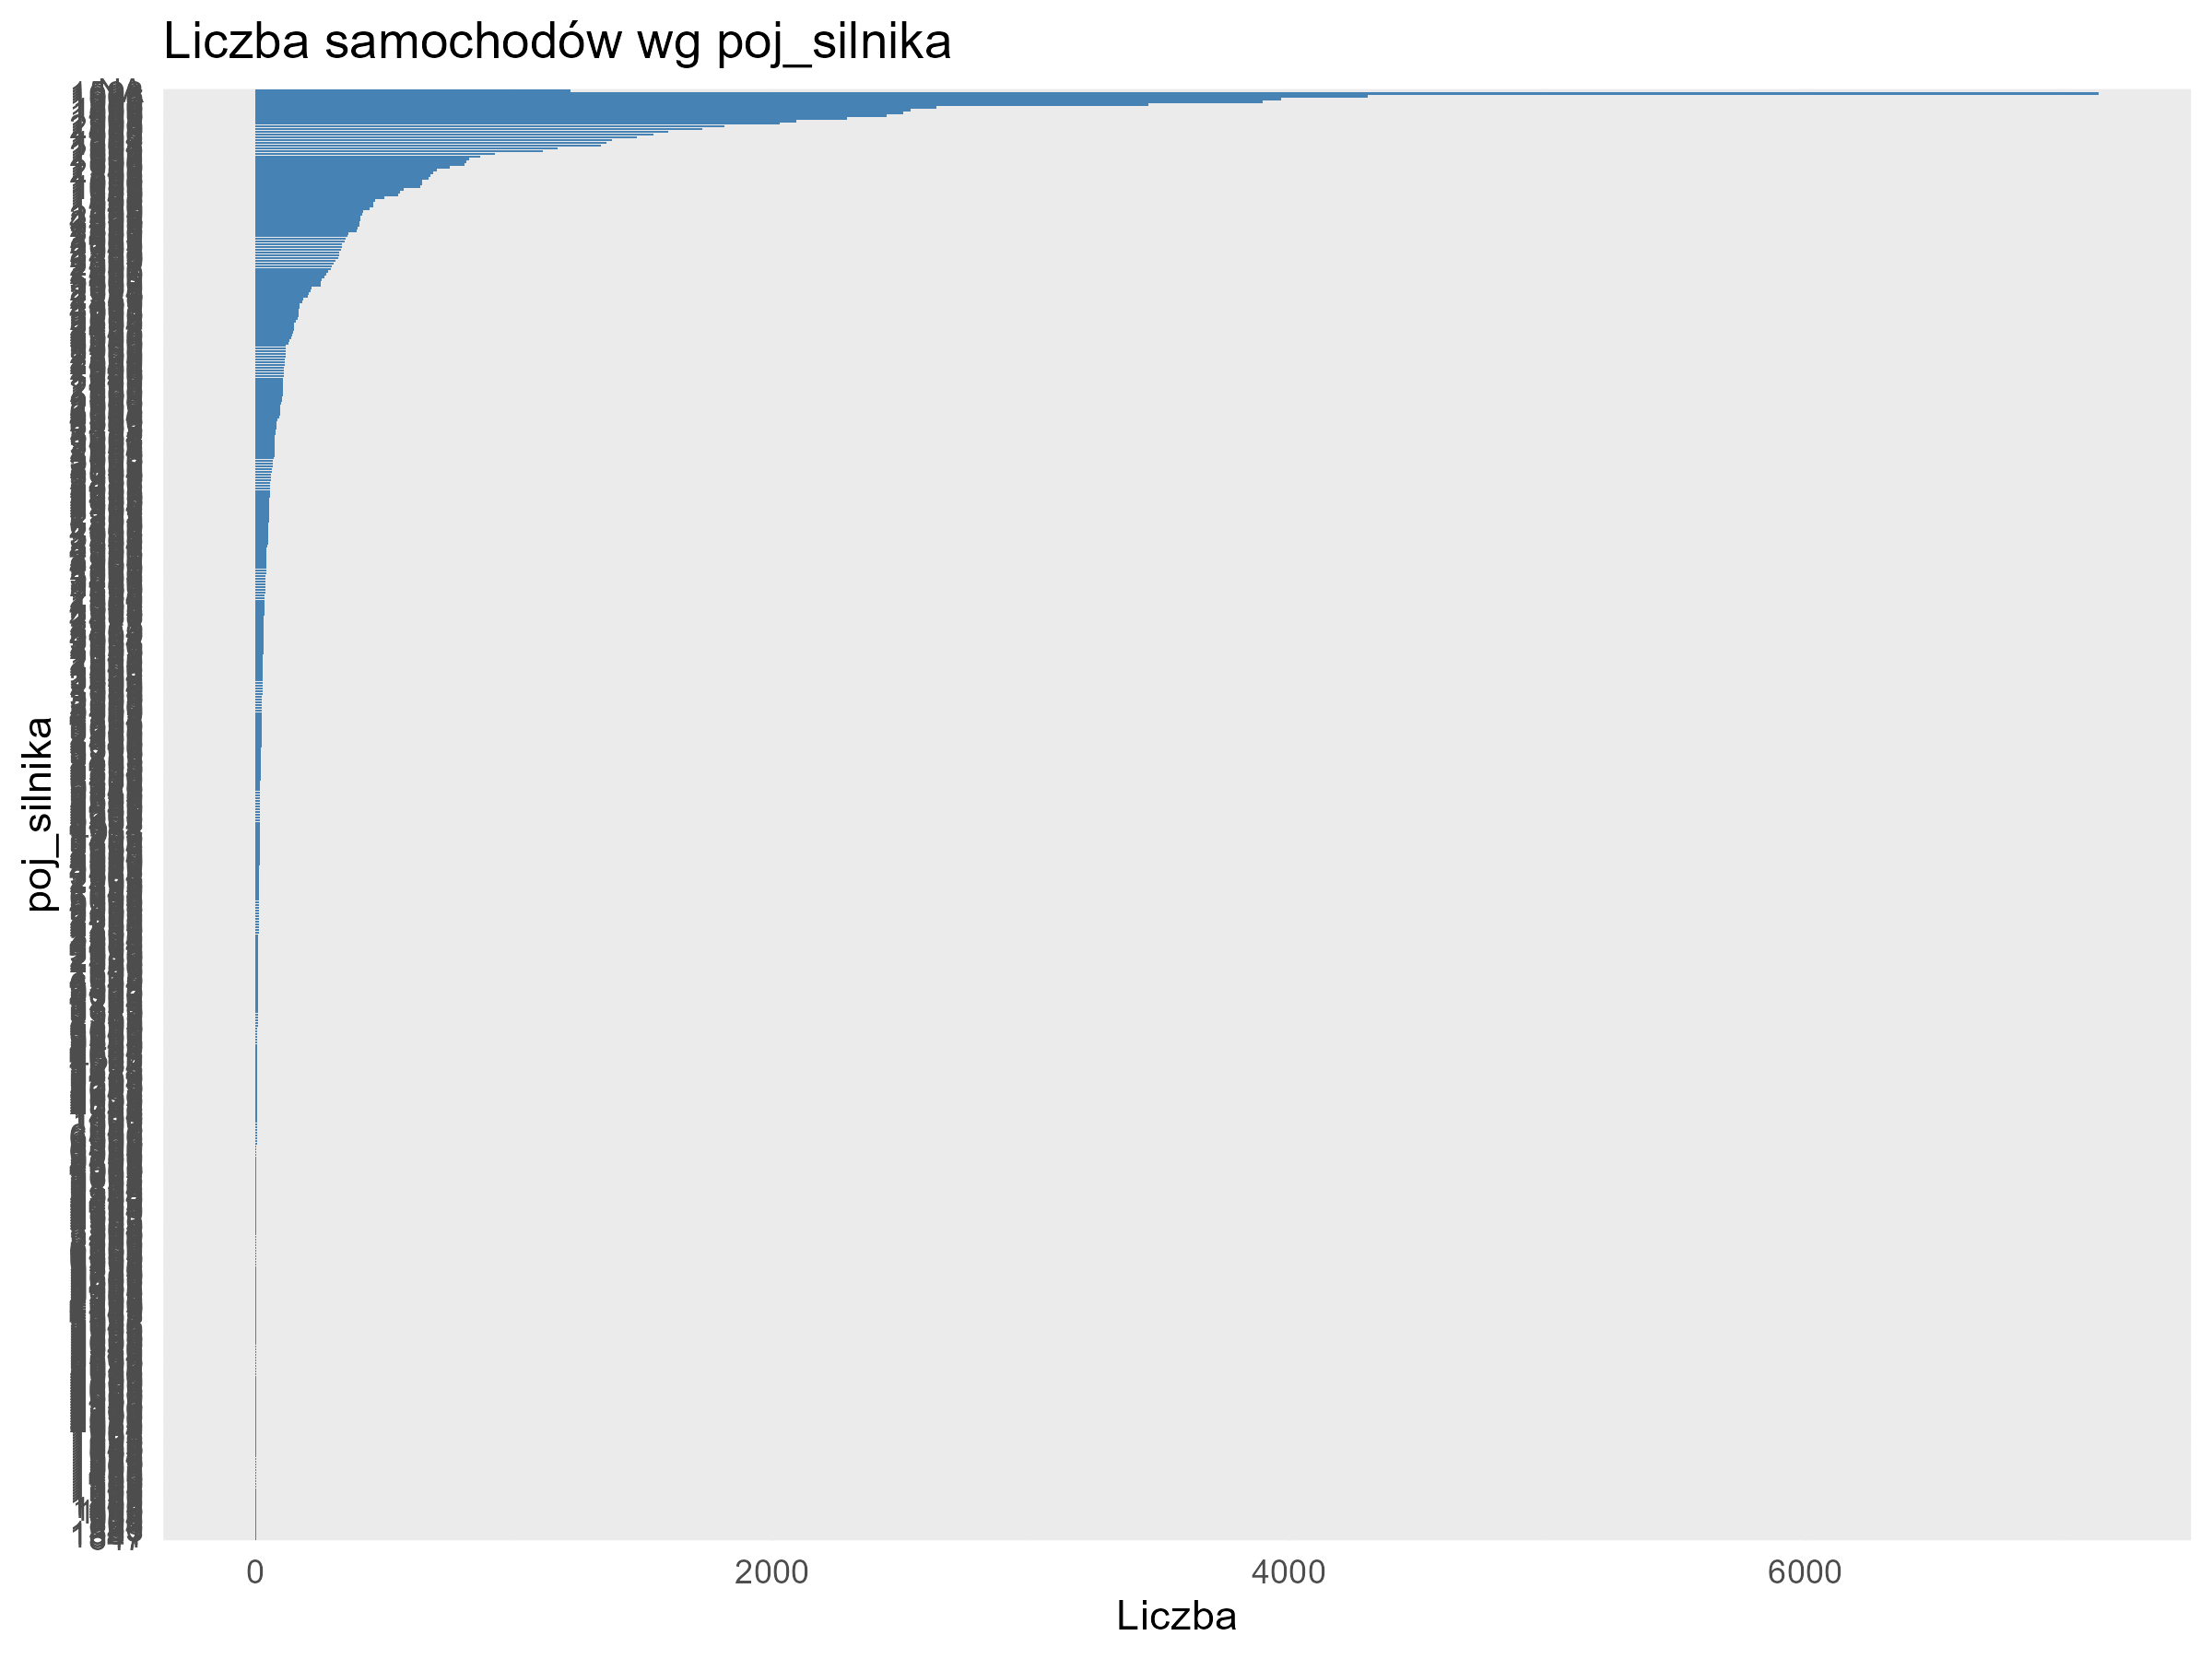
\includegraphics[width=1\linewidth]{analiza/wykres_poj_silnika}

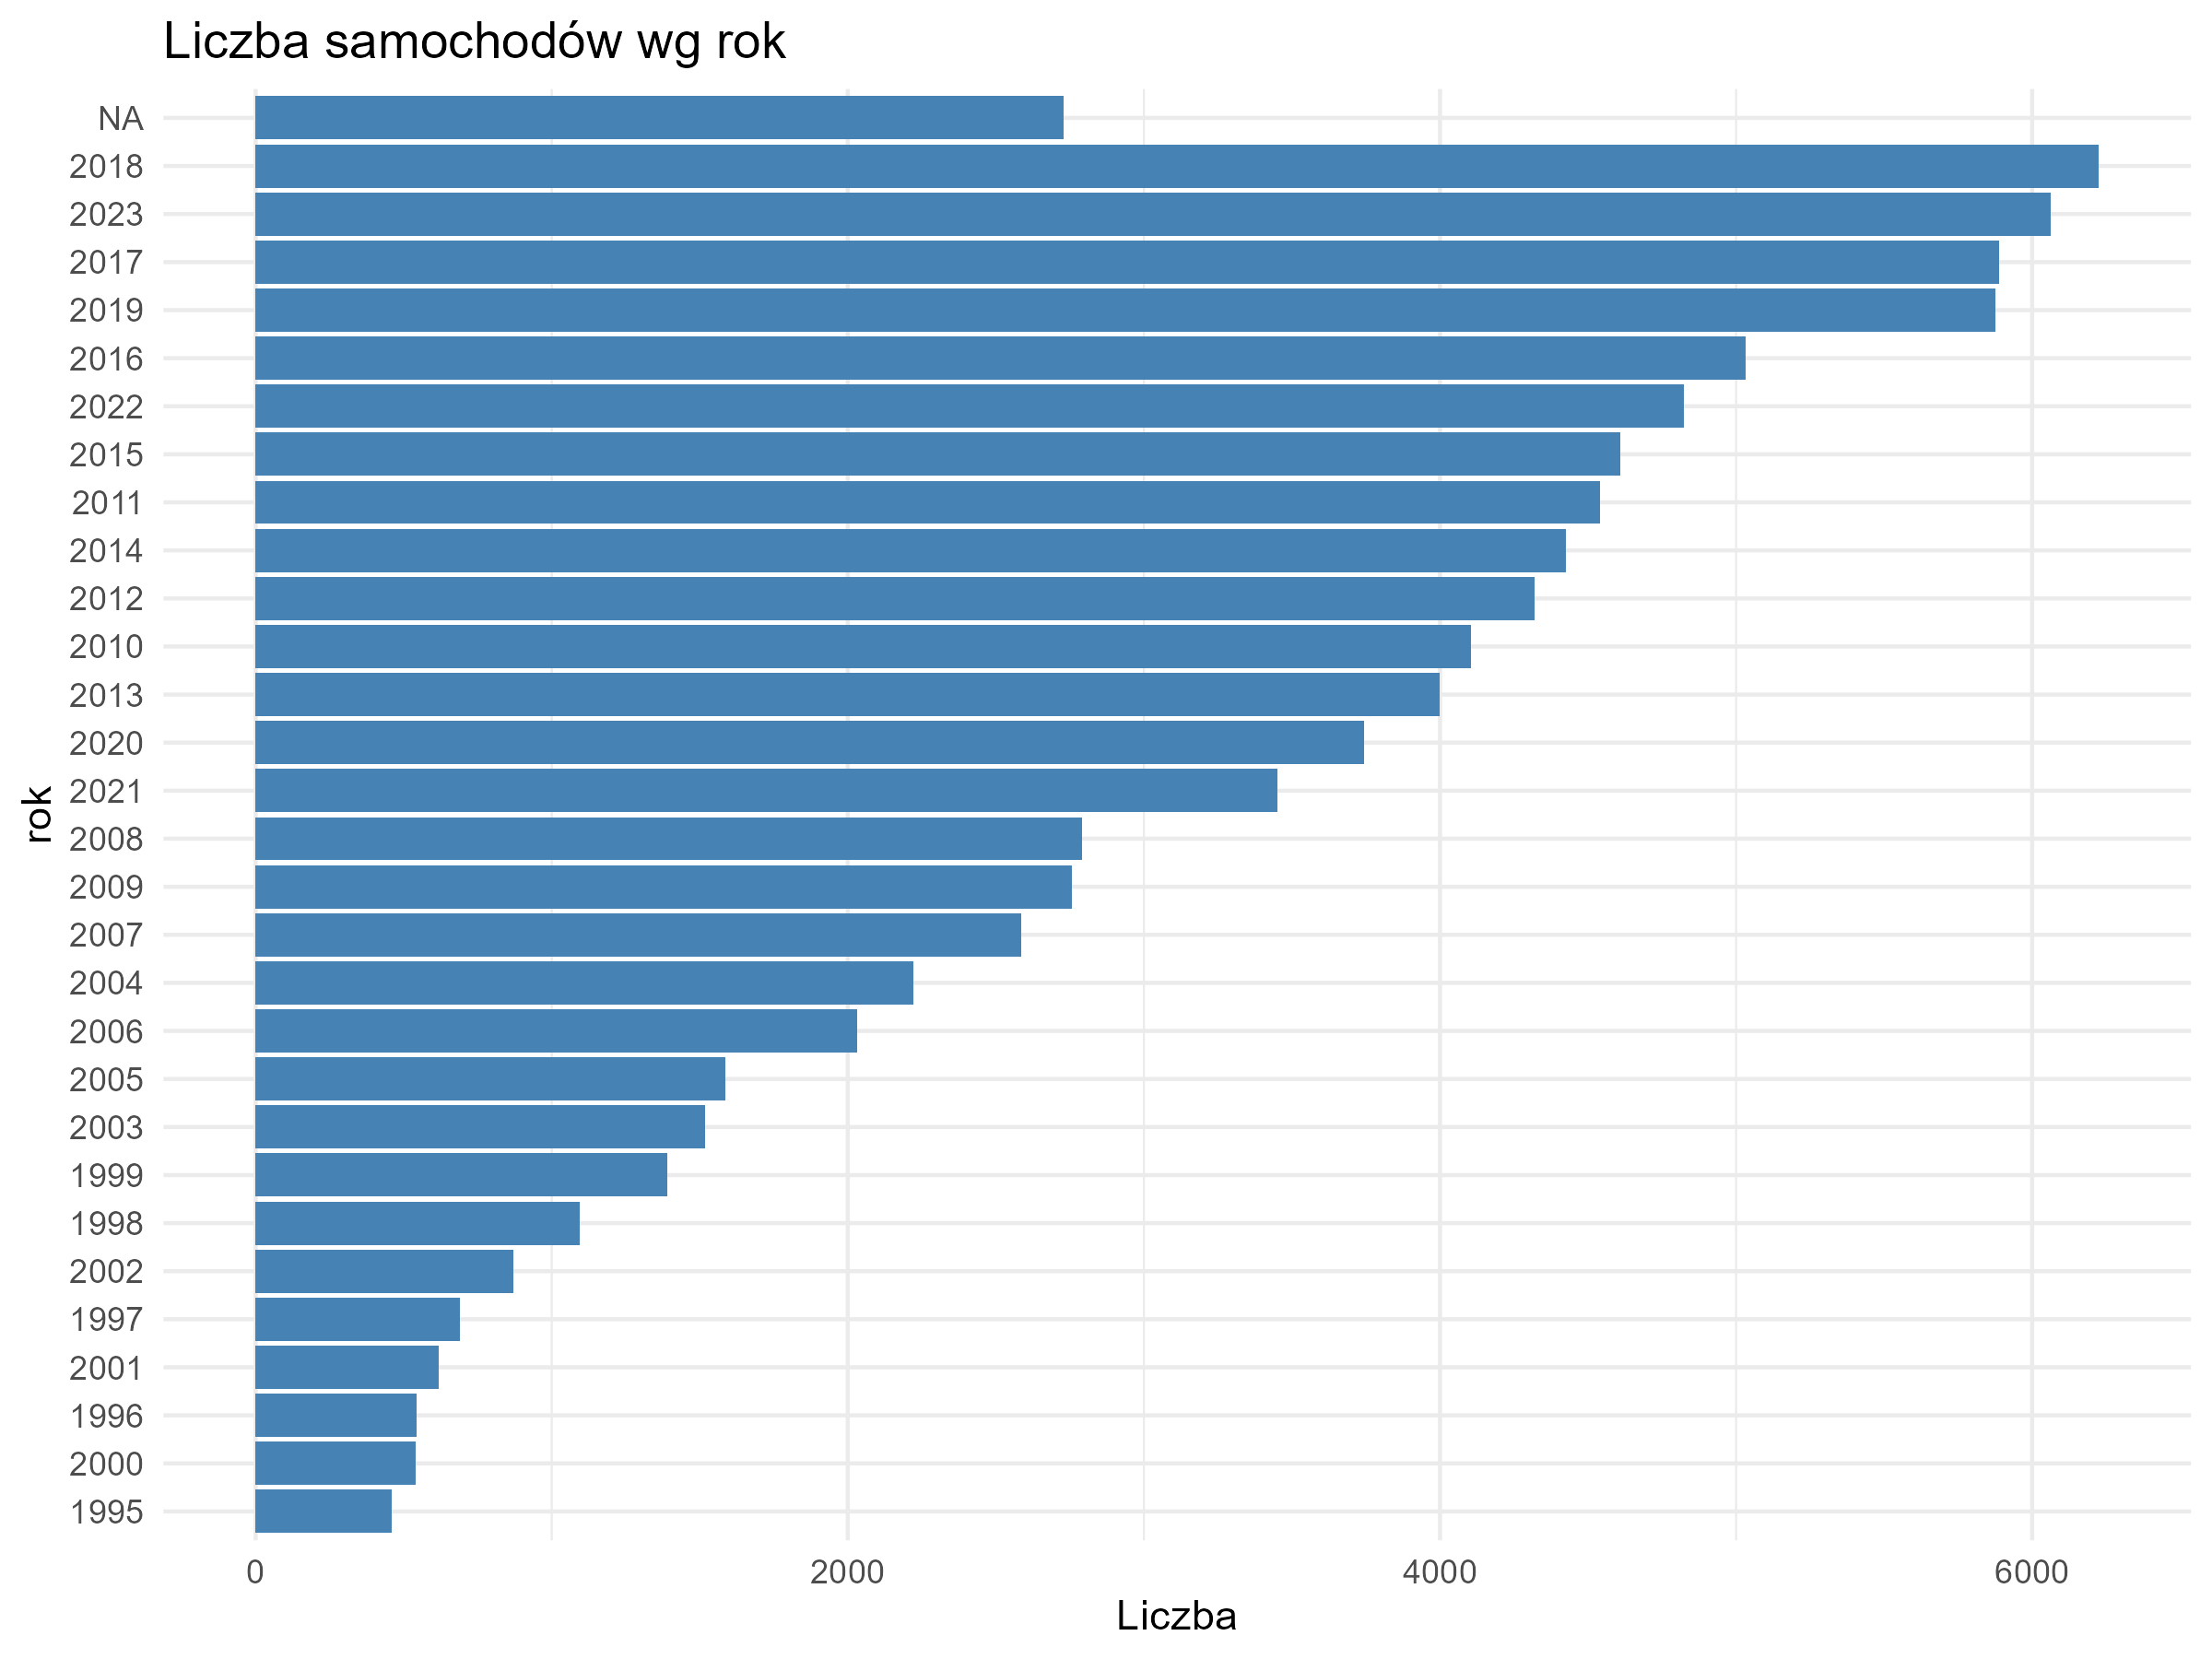
\includegraphics[width=1\linewidth]{analiza/wykres_rok}

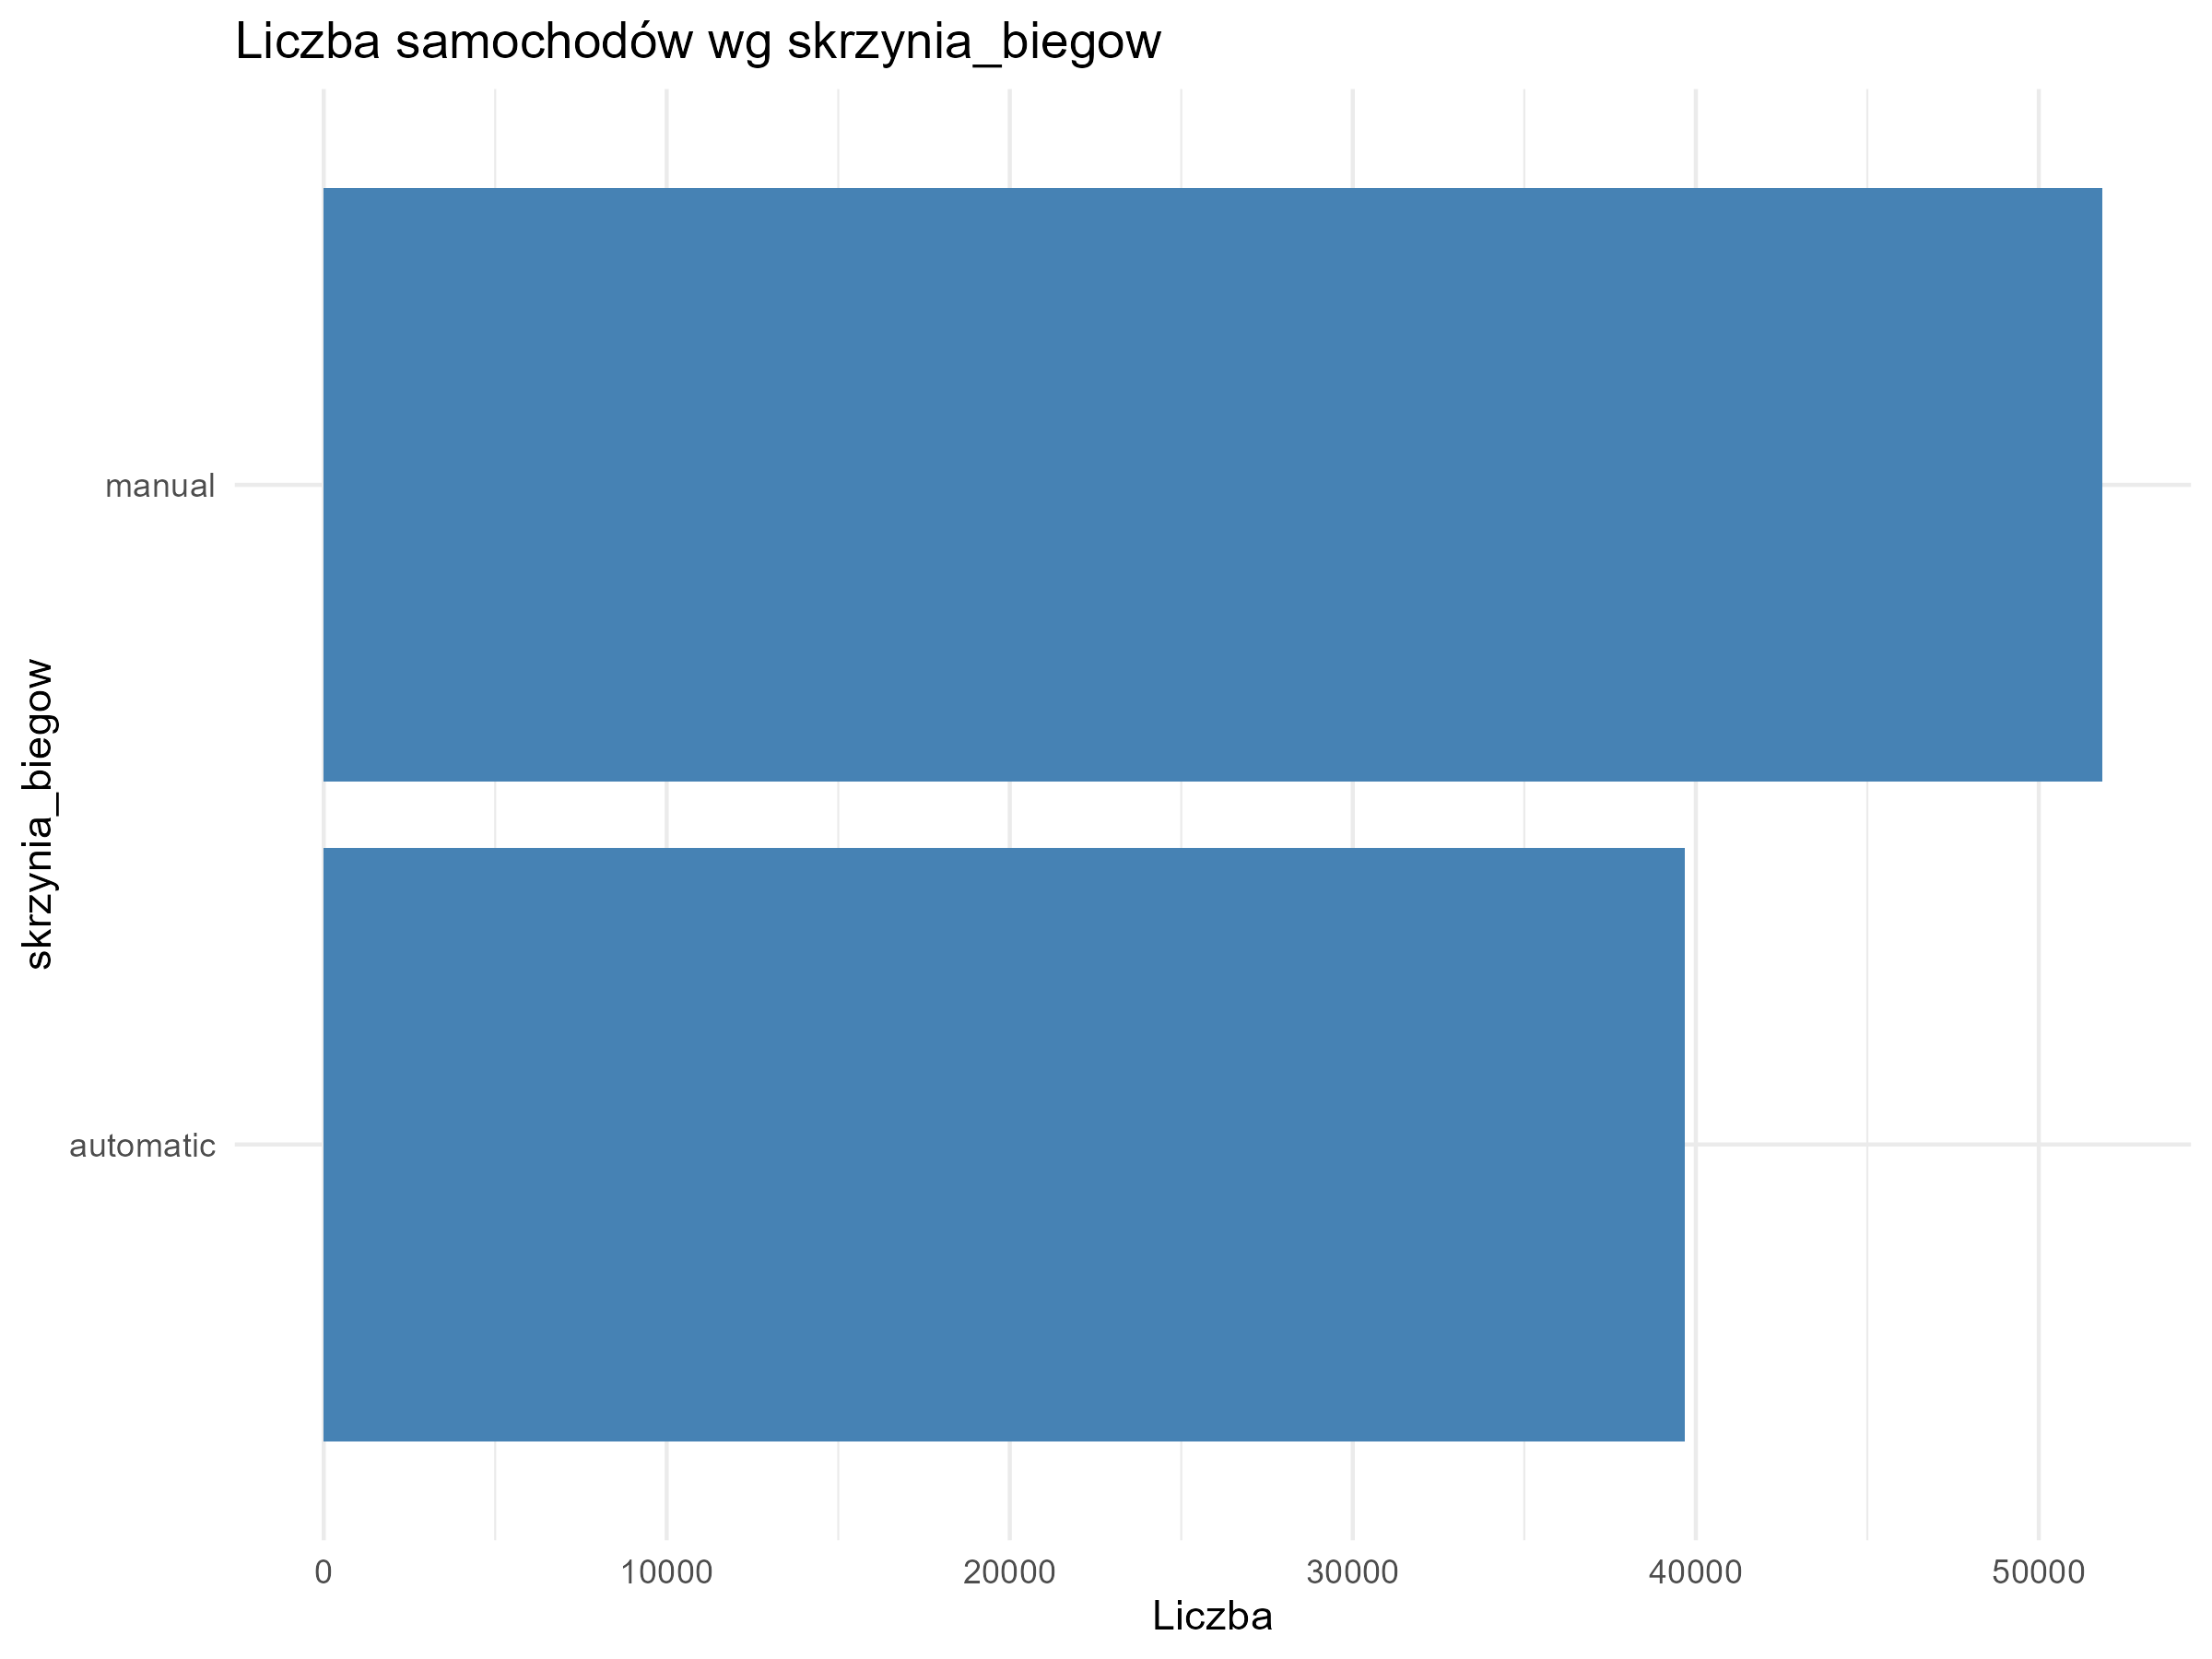
\includegraphics[width=1\linewidth]{analiza/wykres_skrzynia_biegow}

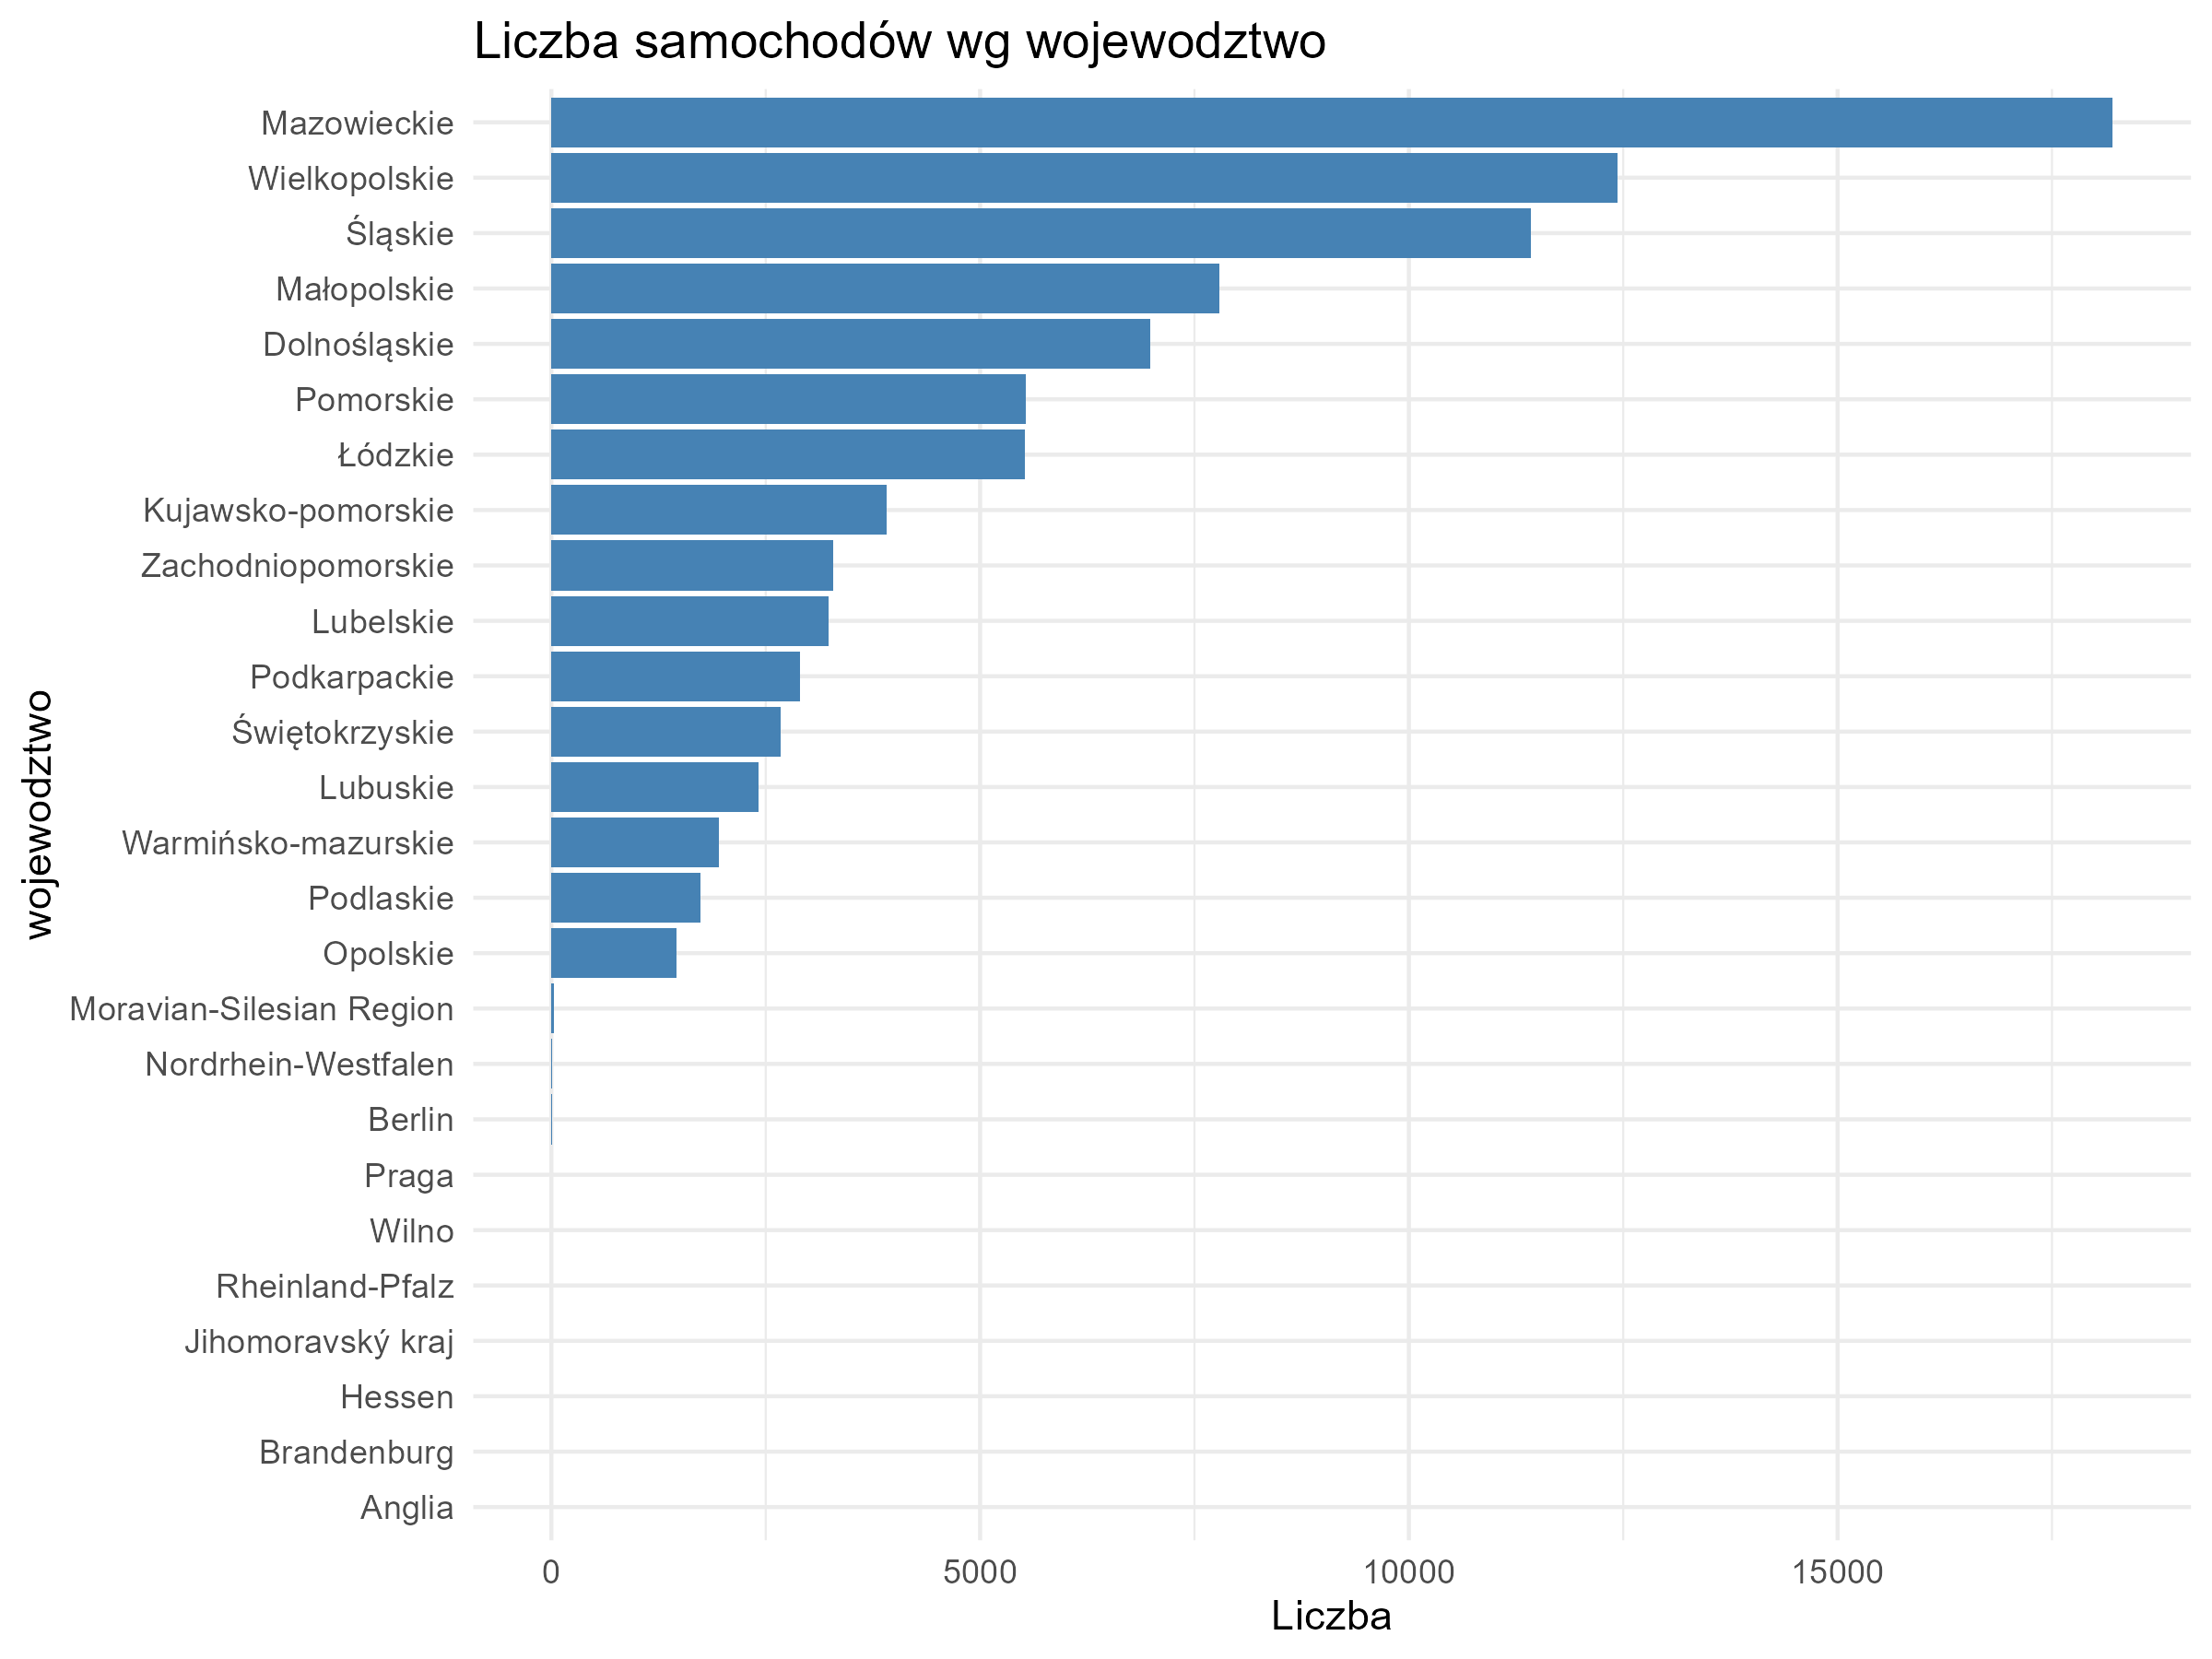
\includegraphics[width=1\linewidth]{analiza/wykres_wojewodztwo}

Z wykresów możemy wywnioskować, że najwięcej ofert na portalu jest dla
marki Volkswagen, a najmniej Lamborghini. Najczęstszymi rodzajami paliwa
są paliwo oraz diesel, natomiast ofert z wodorowym napędem na portalu
nie ma. Najwięcej samochodów zamieszczonych na portalu są 2018 roku
produkcji, natomiast najrzadziej 1995.Więcej ofert jest dla samochodów z
manualną skrzynią biegów niż automatyczną.Mazowieckie województwo jest
liderem pod względem dostępnych ofert.

Ze względu na bardzo dużą liczbę danych dla zmiennyc: model, miasto,
poj\_silnika wygenerowane wykresy są nieczytelne, więc dla nich musimy
zastosować inne metody generowania wykresów.

Dla wykresu dla zmiennej model wygenerujemy 10 najczęściej wybieranych
modeli i dla nich wygenerujemy wykres.

\begin{Shaded}
\begin{Highlighting}[]
\CommentTok{\# Funkcja do tworzenia wykresów top i bottom 10}
\NormalTok{wykres\_top\_bottom }\OtherTok{\textless{}{-}} \ControlFlowTok{function}\NormalTok{(dane, nazwa) \{}
\NormalTok{  top\_10 }\OtherTok{\textless{}{-}}\NormalTok{ dane }\SpecialCharTok{\%\textgreater{}\%} \FunctionTok{top\_n}\NormalTok{(}\DecValTok{10}\NormalTok{, n)}
\NormalTok{  bottom\_10 }\OtherTok{\textless{}{-}}\NormalTok{ dane }\SpecialCharTok{\%\textgreater{}\%} \FunctionTok{top\_n}\NormalTok{(}\SpecialCharTok{{-}}\DecValTok{10}\NormalTok{, n)}
  
\NormalTok{  p1 }\OtherTok{\textless{}{-}} \FunctionTok{ggplot}\NormalTok{(top\_10, }\FunctionTok{aes}\NormalTok{(}\AttributeTok{x =} \FunctionTok{reorder}\NormalTok{(Kategoria, n), }\AttributeTok{y =}\NormalTok{ n)) }\SpecialCharTok{+}
    \FunctionTok{geom\_bar}\NormalTok{(}\AttributeTok{stat =} \StringTok{"identity"}\NormalTok{, }\AttributeTok{fill =} \StringTok{"steelblue"}\NormalTok{) }\SpecialCharTok{+}
    \FunctionTok{coord\_flip}\NormalTok{() }\SpecialCharTok{+}
    \FunctionTok{labs}\NormalTok{(}\AttributeTok{title =} \FunctionTok{paste}\NormalTok{(}\StringTok{"Top 10"}\NormalTok{, nazwa), }\AttributeTok{x =}\NormalTok{ nazwa, }\AttributeTok{y =} \StringTok{"Liczba"}\NormalTok{) }\SpecialCharTok{+}
    \FunctionTok{theme\_minimal}\NormalTok{()}
  
\NormalTok{  p2 }\OtherTok{\textless{}{-}} \FunctionTok{ggplot}\NormalTok{(bottom\_10, }\FunctionTok{aes}\NormalTok{(}\AttributeTok{x =} \FunctionTok{reorder}\NormalTok{(Kategoria, n), }\AttributeTok{y =}\NormalTok{ n)) }\SpecialCharTok{+}
    \FunctionTok{geom\_bar}\NormalTok{(}\AttributeTok{stat =} \StringTok{"identity"}\NormalTok{, }\AttributeTok{fill =} \StringTok{"red"}\NormalTok{) }\SpecialCharTok{+}
    \FunctionTok{coord\_flip}\NormalTok{() }\SpecialCharTok{+}
    \FunctionTok{labs}\NormalTok{(}\AttributeTok{title =} \FunctionTok{paste}\NormalTok{(}\StringTok{"Bottom 10"}\NormalTok{, nazwa), }\AttributeTok{x =}\NormalTok{ nazwa, }\AttributeTok{y =} \StringTok{"Liczba"}\NormalTok{) }\SpecialCharTok{+}
    \FunctionTok{theme\_minimal}\NormalTok{()}
  
  \FunctionTok{return}\NormalTok{(}\FunctionTok{list}\NormalTok{(p1, p2))}
\NormalTok{\}}

\CommentTok{\# Wczytanie danych}
\NormalTok{tabele }\OtherTok{\textless{}{-}} \FunctionTok{lapply}\NormalTok{(tabele, }\ControlFlowTok{function}\NormalTok{(tbl) \{}
  \FunctionTok{colnames}\NormalTok{(tbl) }\OtherTok{\textless{}{-}} \FunctionTok{c}\NormalTok{(}\StringTok{"Kategoria"}\NormalTok{, }\StringTok{"n"}\NormalTok{)}
\NormalTok{  tbl}
\NormalTok{\})}
\NormalTok{wykres\_model }\OtherTok{\textless{}{-}} \FunctionTok{wykres\_top\_bottom}\NormalTok{(tabele[[}\StringTok{"model"}\NormalTok{]], }\StringTok{"Model"}\NormalTok{)}
\FunctionTok{ggsave}\NormalTok{(}\StringTok{"wykres\_top\_model.png"}\NormalTok{, }\AttributeTok{plot =}\NormalTok{ ploty\_model[[}\DecValTok{1}\NormalTok{]], }\AttributeTok{width =} \DecValTok{8}\NormalTok{, }\AttributeTok{height =} \DecValTok{6}\NormalTok{)}
\end{Highlighting}
\end{Shaded}

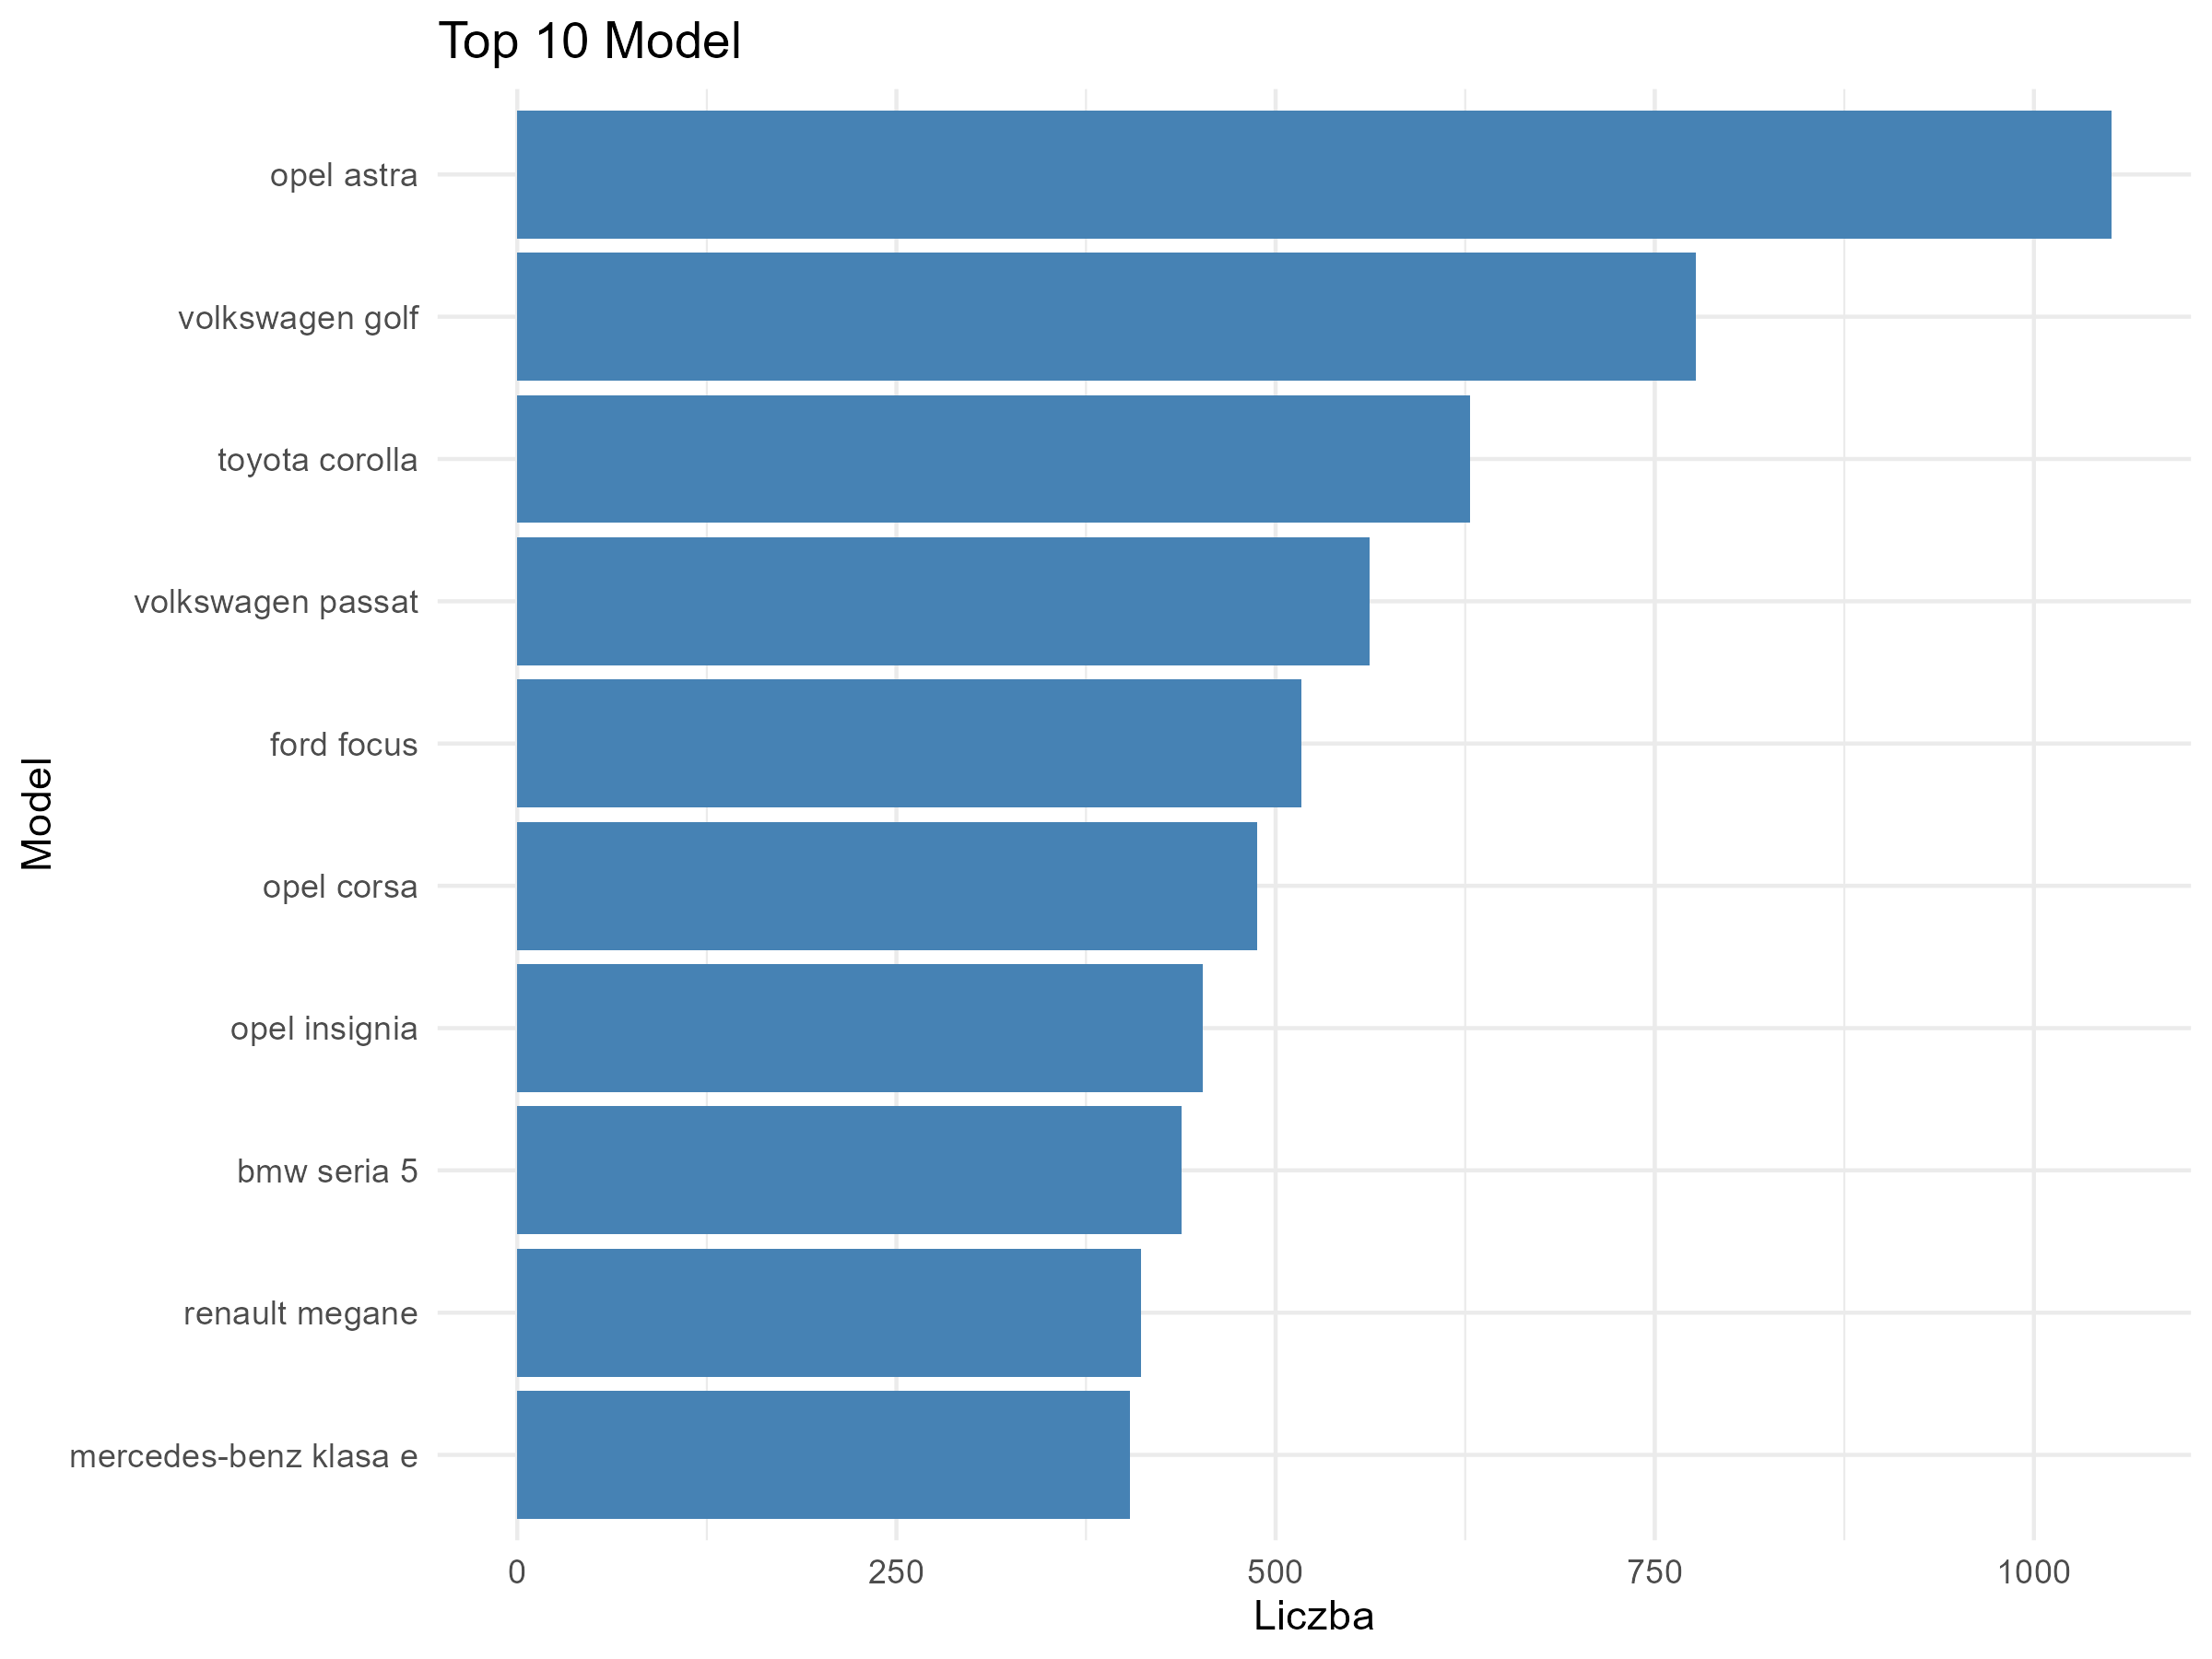
\includegraphics[width=1\linewidth]{analiza/wykres_top_model}

Opel astra jest najczęściej sprzedawanym modelem.

Dla lepszego zrozumienia danych sprawdziliśmy podstawowe statystyki dla
zmiennych numerycznych.

\begin{Shaded}
\begin{Highlighting}[]
\CommentTok{\# 3. Statystyki opisowe}
\NormalTok{statystyki\_opisowe }\OtherTok{\textless{}{-}}\NormalTok{ dane }\SpecialCharTok{\%\textgreater{}\%}
  \FunctionTok{summarise}\NormalTok{(}
    \AttributeTok{MinCena =} \FunctionTok{min}\NormalTok{(cena\_zl, }\AttributeTok{na.rm =} \ConstantTok{TRUE}\NormalTok{),}
    \AttributeTok{SredniaCena =} \FunctionTok{mean}\NormalTok{(cena\_zl, }\AttributeTok{na.rm =} \ConstantTok{TRUE}\NormalTok{),}
    \AttributeTok{MedianaCena =} \FunctionTok{median}\NormalTok{(cena\_zl, }\AttributeTok{na.rm =} \ConstantTok{TRUE}\NormalTok{),}
    \AttributeTok{MaxCena =} \FunctionTok{max}\NormalTok{(cena\_zl, }\AttributeTok{na.rm =} \ConstantTok{TRUE}\NormalTok{),}
    \AttributeTok{OdchylenieCena =} \FunctionTok{sd}\NormalTok{(cena\_zl, }\AttributeTok{na.rm =} \ConstantTok{TRUE}\NormalTok{),}
    \AttributeTok{IQR\_Cena =} \FunctionTok{IQR}\NormalTok{(cena\_zl, }\AttributeTok{na.rm =} \ConstantTok{TRUE}\NormalTok{),}
    \AttributeTok{MinPrzebieg =} \FunctionTok{min}\NormalTok{(przebieg\_w\_km, }\AttributeTok{na.rm =} \ConstantTok{TRUE}\NormalTok{),}
    \AttributeTok{SredniPrzebieg =} \FunctionTok{mean}\NormalTok{(przebieg\_w\_km, }\AttributeTok{na.rm =} \ConstantTok{TRUE}\NormalTok{),}
    \AttributeTok{MaxPrzebieg =} \FunctionTok{max}\NormalTok{(przebieg\_w\_km, }\AttributeTok{na.rm =} \ConstantTok{TRUE}\NormalTok{),}
    \AttributeTok{MinRok =} \FunctionTok{min}\NormalTok{(rok, }\AttributeTok{na.rm =} \ConstantTok{TRUE}\NormalTok{),}
    \AttributeTok{MaxRok =} \FunctionTok{max}\NormalTok{(rok, }\AttributeTok{na.rm =} \ConstantTok{TRUE}\NormalTok{)}
\NormalTok{  )}
\FunctionTok{print}\NormalTok{(statystyki\_opisowe)}

\CommentTok{\# 4. Wyświetlenie raportu i wykresu dla statystyk opisowych}
\NormalTok{statystyki\_opisowe }\OtherTok{\textless{}{-}} \FunctionTok{data.frame}\NormalTok{(}
  \AttributeTok{Statystyka =} \FunctionTok{names}\NormalTok{(statystyki\_opisowe),}
\NormalTok{  Wartość }\OtherTok{=} \FunctionTok{unlist}\NormalTok{(statystyki\_opisowe)}
\NormalTok{)}
\NormalTok{p\_statystyki }\OtherTok{\textless{}{-}} \FunctionTok{ggplot}\NormalTok{(statystyki\_opisowe, }\FunctionTok{aes}\NormalTok{(}\AttributeTok{x =}\NormalTok{ Statystyka, }\AttributeTok{y =}\NormalTok{ Wartość)) }\SpecialCharTok{+}
  \FunctionTok{geom\_col}\NormalTok{(}\AttributeTok{fill =} \StringTok{"blue"}\NormalTok{) }\SpecialCharTok{+}
  \FunctionTok{labs}\NormalTok{(}
    \AttributeTok{title =} \StringTok{"Podstawowe statystyki opisowe"}\NormalTok{,}
    \AttributeTok{x =} \StringTok{"Statystyka"}\NormalTok{,}
    \AttributeTok{y =} \StringTok{"Wartość"}
\NormalTok{  ) }\SpecialCharTok{+}
  \FunctionTok{theme\_minimal}\NormalTok{() }\SpecialCharTok{+}
  \FunctionTok{theme}\NormalTok{(}\AttributeTok{axis.text.x =} \FunctionTok{element\_text}\NormalTok{(}\AttributeTok{angle =} \DecValTok{45}\NormalTok{, }\AttributeTok{hjust =} \DecValTok{1}\NormalTok{))}
\FunctionTok{ggsave}\NormalTok{(}\StringTok{"statystyki\_opisowe.png"}\NormalTok{, }\AttributeTok{plot =}\NormalTok{ p\_statystyki, }\AttributeTok{width =} \DecValTok{8}\NormalTok{, }\AttributeTok{height =} \DecValTok{6}\NormalTok{)}
\end{Highlighting}
\end{Shaded}

Najniższa cena na portalu o 1111 zł, średnia cena za samochód to
84146,29 zł, mediana natiomiast plasuje się na poziomie 49900.

W celu zbadania zależności pomiędzy zmiennymi zależnymi tworzymy macierz
korrelacji oraz odpowiedni wykres

\begin{Shaded}
\begin{Highlighting}[]
\NormalTok{num\_cols }\OtherTok{\textless{}{-}}\NormalTok{ dane }\SpecialCharTok{\%\textgreater{}\%} \FunctionTok{select}\NormalTok{(}\FunctionTok{where}\NormalTok{(is.numeric)) }\CommentTok{\# Wybierz kolumny numeryczne}
\NormalTok{cor\_matrix }\OtherTok{\textless{}{-}} \FunctionTok{cor}\NormalTok{(num\_cols, }\AttributeTok{use =} \StringTok{"complete.obs"}\NormalTok{)}
\FunctionTok{print}\NormalTok{(cor\_matrix)}
\FunctionTok{png}\NormalTok{(}\StringTok{"wykres\_korelacji.png"}\NormalTok{, }\AttributeTok{width =} \DecValTok{800}\NormalTok{, }\AttributeTok{height =} \DecValTok{800}\NormalTok{) }\CommentTok{\# Utwórz plik PNG}
\FunctionTok{corrplot}\NormalTok{(cor\_matrix, }\AttributeTok{method =} \StringTok{"circle"}\NormalTok{, }\AttributeTok{type =} \StringTok{"lower"}\NormalTok{, }\AttributeTok{tl.col =} \StringTok{"black"}\NormalTok{, }\AttributeTok{tl.srt =} \DecValTok{45}\NormalTok{)}
\FunctionTok{dev.off}\NormalTok{()}
\end{Highlighting}
\end{Shaded}

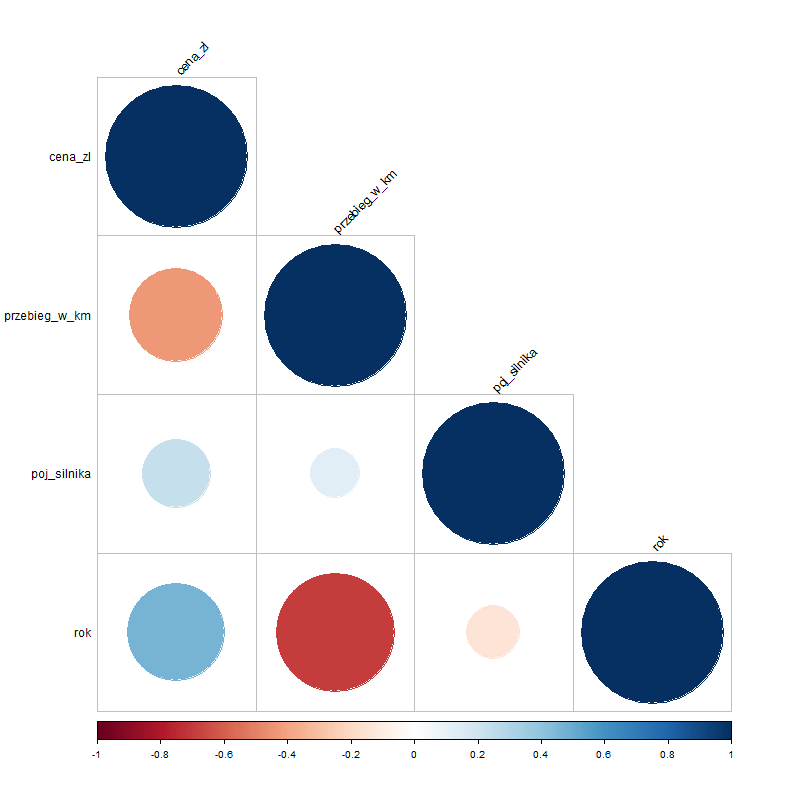
\includegraphics[width=1\linewidth]{analiza/wykres_korelacji}

Cena wykazuje umiarkowaną korrelację z rokiem produkcji (r=0,47), co
sugeruje, że nowsze samochody są droższe. Natomiast niską korrelację z
pojemnością silnika oraz ujemną korelację z przebiegiem, co oznacza, że
każdy dodatkowy kilometr obniża cenę samochodu. Przebieg ma silną
korrelację z rokiem produkcji, co jest dosyć oczywistym stwierdzeniem,
że starsze samochody mają większy przebieg. Pojemność silnika wykazuje
bardzo słabe korelacje z innymi zmiennymi. Rok produkcji jest silnie
skorelowany z ceną i bardzo silnie ujemnie z przebiegiem, co podkreśla
znaczenie wieku samochodu w kontekście jego wartości i użytkowania.
Najistotniejsze czynniki wpływające na cenę samochodu to rok produkcji i
przebieg, co zgadza się z intuicyjnym podejściem do wyceny pojazdów.
Pojemność silnika ma stosunkowo niewielki wpływ na cenę, a jej korelacje
z innymi zmiennymi są słabe.

Testy statystyczne Kolejną częścią raportu jest przeprowadzenie
przykładowych testów statystycznych

W celu przedstawienia współzależności pomiędzy dwiema zmiennymi
kategorycznymi w postaci tabeli oraz sprawdzenia istnienia takowej
współzależności stworzyliśmy tabele kontyngencji oraz przeprowadziliśmy
test chi-kwadrat. Sprawdziliśmy czy wybór marki zależy od województwa,
typ skrzyni biegu zależy od rodzaju paliwa, czy wybór modelu zależy od
miasta.

\section{6. Testy statystyczne}\label{testy-statystyczne}

\section{Tabela kontyngencji i test
chi-kwadrat}\label{tabela-kontyngencji-i-test-chi-kwadrat}

\begin{Shaded}
\begin{Highlighting}[]
\NormalTok{tabela\_marka\_wojewodztwo }\OtherTok{\textless{}{-}} \FunctionTok{table}\NormalTok{(dane}\SpecialCharTok{$}\NormalTok{marka, dane}\SpecialCharTok{$}\NormalTok{wojewodztwo)}
\FunctionTok{print}\NormalTok{(tabela\_marka\_wojewodztwo)}
\NormalTok{chi\_sq\_result }\OtherTok{\textless{}{-}} \FunctionTok{chisq.test}\NormalTok{(tabela\_marka\_wojewodztwo)}
\FunctionTok{print}\NormalTok{(chi\_sq\_result)}
\NormalTok{tabela\_paliwo\_skrzynia }\OtherTok{\textless{}{-}} \FunctionTok{table}\NormalTok{(dane}\SpecialCharTok{$}\NormalTok{paliwo, dane}\SpecialCharTok{$}\NormalTok{skrzynia\_biegow)}
\FunctionTok{print}\NormalTok{(tabela\_paliwo\_skrzynia)}
\NormalTok{chi\_sq\_result1 }\OtherTok{\textless{}{-}} \FunctionTok{chisq.test}\NormalTok{(tabela\_paliwo\_skrzynia )}
\FunctionTok{print}\NormalTok{(chi\_sq\_result1)}
\NormalTok{tabela\_model\_miasto }\OtherTok{\textless{}{-}} \FunctionTok{table}\NormalTok{(dane}\SpecialCharTok{$}\NormalTok{model, dane}\SpecialCharTok{$}\NormalTok{miasto)}
\FunctionTok{print}\NormalTok{(tabela\_model\_miasto)}
\NormalTok{chi\_sq\_result2 }\OtherTok{\textless{}{-}} \FunctionTok{chisq.test}\NormalTok{(tabela\_model\_miasto )}
\FunctionTok{print}\NormalTok{(chi\_sq\_result2)}
\FunctionTok{png}\NormalTok{(}\StringTok{"mozaikowy\_paliwo\_skrzynia.png"}\NormalTok{, }\AttributeTok{width =} \DecValTok{800}\NormalTok{, }\AttributeTok{height =} \DecValTok{600}\NormalTok{)}
\FunctionTok{mosaicplot}\NormalTok{(tabela\_paliwo\_skrzynia, }
           \AttributeTok{main =} \StringTok{"Relacja między rodzajem paliwa a skrzynią biegów"}\NormalTok{, }
           \AttributeTok{color =} \ConstantTok{TRUE}\NormalTok{, }
           \AttributeTok{shade =} \ConstantTok{TRUE}\NormalTok{, }
           \AttributeTok{las =} \DecValTok{1}\NormalTok{, }
           \AttributeTok{cex.axis =} \FloatTok{0.9}\NormalTok{) }
\FunctionTok{dev.off}\NormalTok{()}
\end{Highlighting}
\end{Shaded}

Statystyka testowa (X-squared) = 5174.1 jest bardzo wysoka. Wskazuje to
na dużą różnicę między obserwowaną a oczekiwaną liczbą w tabeli
kontyngencji, co sugeruje potencjalną zależność między zmiennymi.
Stopnie swobody (df) = 1050 oznacza liczbę swobody, która zależy od
liczby kategorii obu zmiennych. Wysoka liczba stopni swobody sugeruje,
że jedna lub obie zmienne mają wiele kategorii. Wartość p
(p-value):p\textless2.2×10 −16, czyli wartość p jest znacznie mniejsza
niż typowy poziom istotności. Oznacza to, że istnieje statystycznie
istotna zależność między marką a województwem. A więc przyjmuje hipotezę
o zależności wyboru marki od miejsca zamieszkania(województwo).
Wygenerowaliśmy również przykładowy wykres mozaikowy do zależności
rodzaju skrzyni biegów od rodzaju paliwa. Istnieje statystycznie istotna
zależność między rodzajem paliwa a typem skrzyni biegów. Wynik testu
sugeruje, że niektóre rodzaje paliwa są bardziej związane z konkretnymi
typami skrzyń biegów. Skrzynie automatyczne są bardziej popularne w
pojazdach z określonym rodzajem paliwa (np. elektryczne lub hybrydowe).
Skrzynie manualne częściej występują w pojazdach z silnikami
spalinowymi. Wynikiem testu chi-kwadrat dla zależności wyboru modelu
samochodu są bardzo duże stopnie swobody, co oznacza zbyt wielką ilość
kategorii

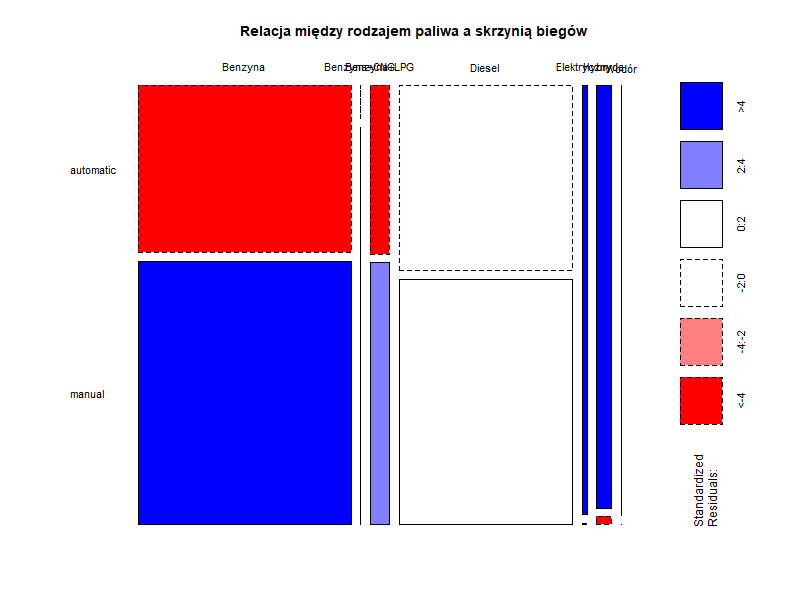
\includegraphics[width=1\linewidth]{analiza/mozaikowy_paliwo_skrzynia}

Kolejnym testem jest test proporcji, żeby sprawdzić rozłożenie róznych
zmiennych. Sprawdzimy różnice pod względem liczby samochodów w różnych
wojewóztwach

\begin{Shaded}
\begin{Highlighting}[]
\CommentTok{\# Testowanie proporcji}
\NormalTok{prop\_table }\OtherTok{\textless{}{-}} \FunctionTok{prop.table}\NormalTok{(}\FunctionTok{table}\NormalTok{(dane}\SpecialCharTok{$}\NormalTok{wojewodztwo))}
\NormalTok{test\_proporcji }\OtherTok{\textless{}{-}} \FunctionTok{chisq.test}\NormalTok{(}\FunctionTok{table}\NormalTok{(dane}\SpecialCharTok{$}\NormalTok{wojewodztwo))}
\FunctionTok{print}\NormalTok{(test\_proporcji)}

\CommentTok{\# Wizualizacja proporcji}
\NormalTok{proporcje }\OtherTok{\textless{}{-}} \FunctionTok{ggplot}\NormalTok{(}\FunctionTok{as.data.frame}\NormalTok{(prop\_table), }\FunctionTok{aes}\NormalTok{(}\AttributeTok{x =}\NormalTok{ Var1, }\AttributeTok{y =}\NormalTok{ Freq)) }\SpecialCharTok{+}
  \FunctionTok{geom\_bar}\NormalTok{(}\AttributeTok{stat =} \StringTok{"identity"}\NormalTok{, }\AttributeTok{fill =} \StringTok{"steelblue"}\NormalTok{) }\SpecialCharTok{+}
  \FunctionTok{labs}\NormalTok{(}\AttributeTok{title =} \StringTok{"Proporcje samochodów w województwach"}\NormalTok{, }\AttributeTok{x =} \StringTok{"Województwo"}\NormalTok{, }\AttributeTok{y =} \StringTok{"Proporcja"}\NormalTok{) }\SpecialCharTok{+}
  \FunctionTok{theme\_minimal}\NormalTok{() }\SpecialCharTok{+} \FunctionTok{theme}\NormalTok{(}\AttributeTok{axis.text.x =} \FunctionTok{element\_text}\NormalTok{(}\AttributeTok{angle =} \DecValTok{45}\NormalTok{, }\AttributeTok{hjust =} \DecValTok{1}\NormalTok{))}
\FunctionTok{ggsave}\NormalTok{(}\StringTok{"wykres\_proporcje.png"}\NormalTok{, }\AttributeTok{plot =}\NormalTok{ proporcje, }\AttributeTok{width =} \DecValTok{10}\NormalTok{, }\AttributeTok{height =} \DecValTok{6}\NormalTok{, }\AttributeTok{dpi =} \DecValTok{300}\NormalTok{)}
\end{Highlighting}
\end{Shaded}

Wyniki testu: Statystyka testowa 151,161 jest bardzo wysoka, co wskazuje
na istotne różnice między obserwowaną a oczekiwaną liczbą samochodów w
województwach. Stopnie swobody 25, co oznacza, że test uwzględnia
rozkład samochodów w 26 województwach. Wartość p\textless2.2×10 −16, co
oznacza statystycznie istotne różnice w proporcjach. Rozkład samochodów
w województwach nie jest równomierny. Województwa różnią się znacząco
pod względem liczby samochodów. Różnice te mogą wynikać z gęstości
zaludnienia, poziomu urbanizacji, dostępności określonych marek lub
modeli.

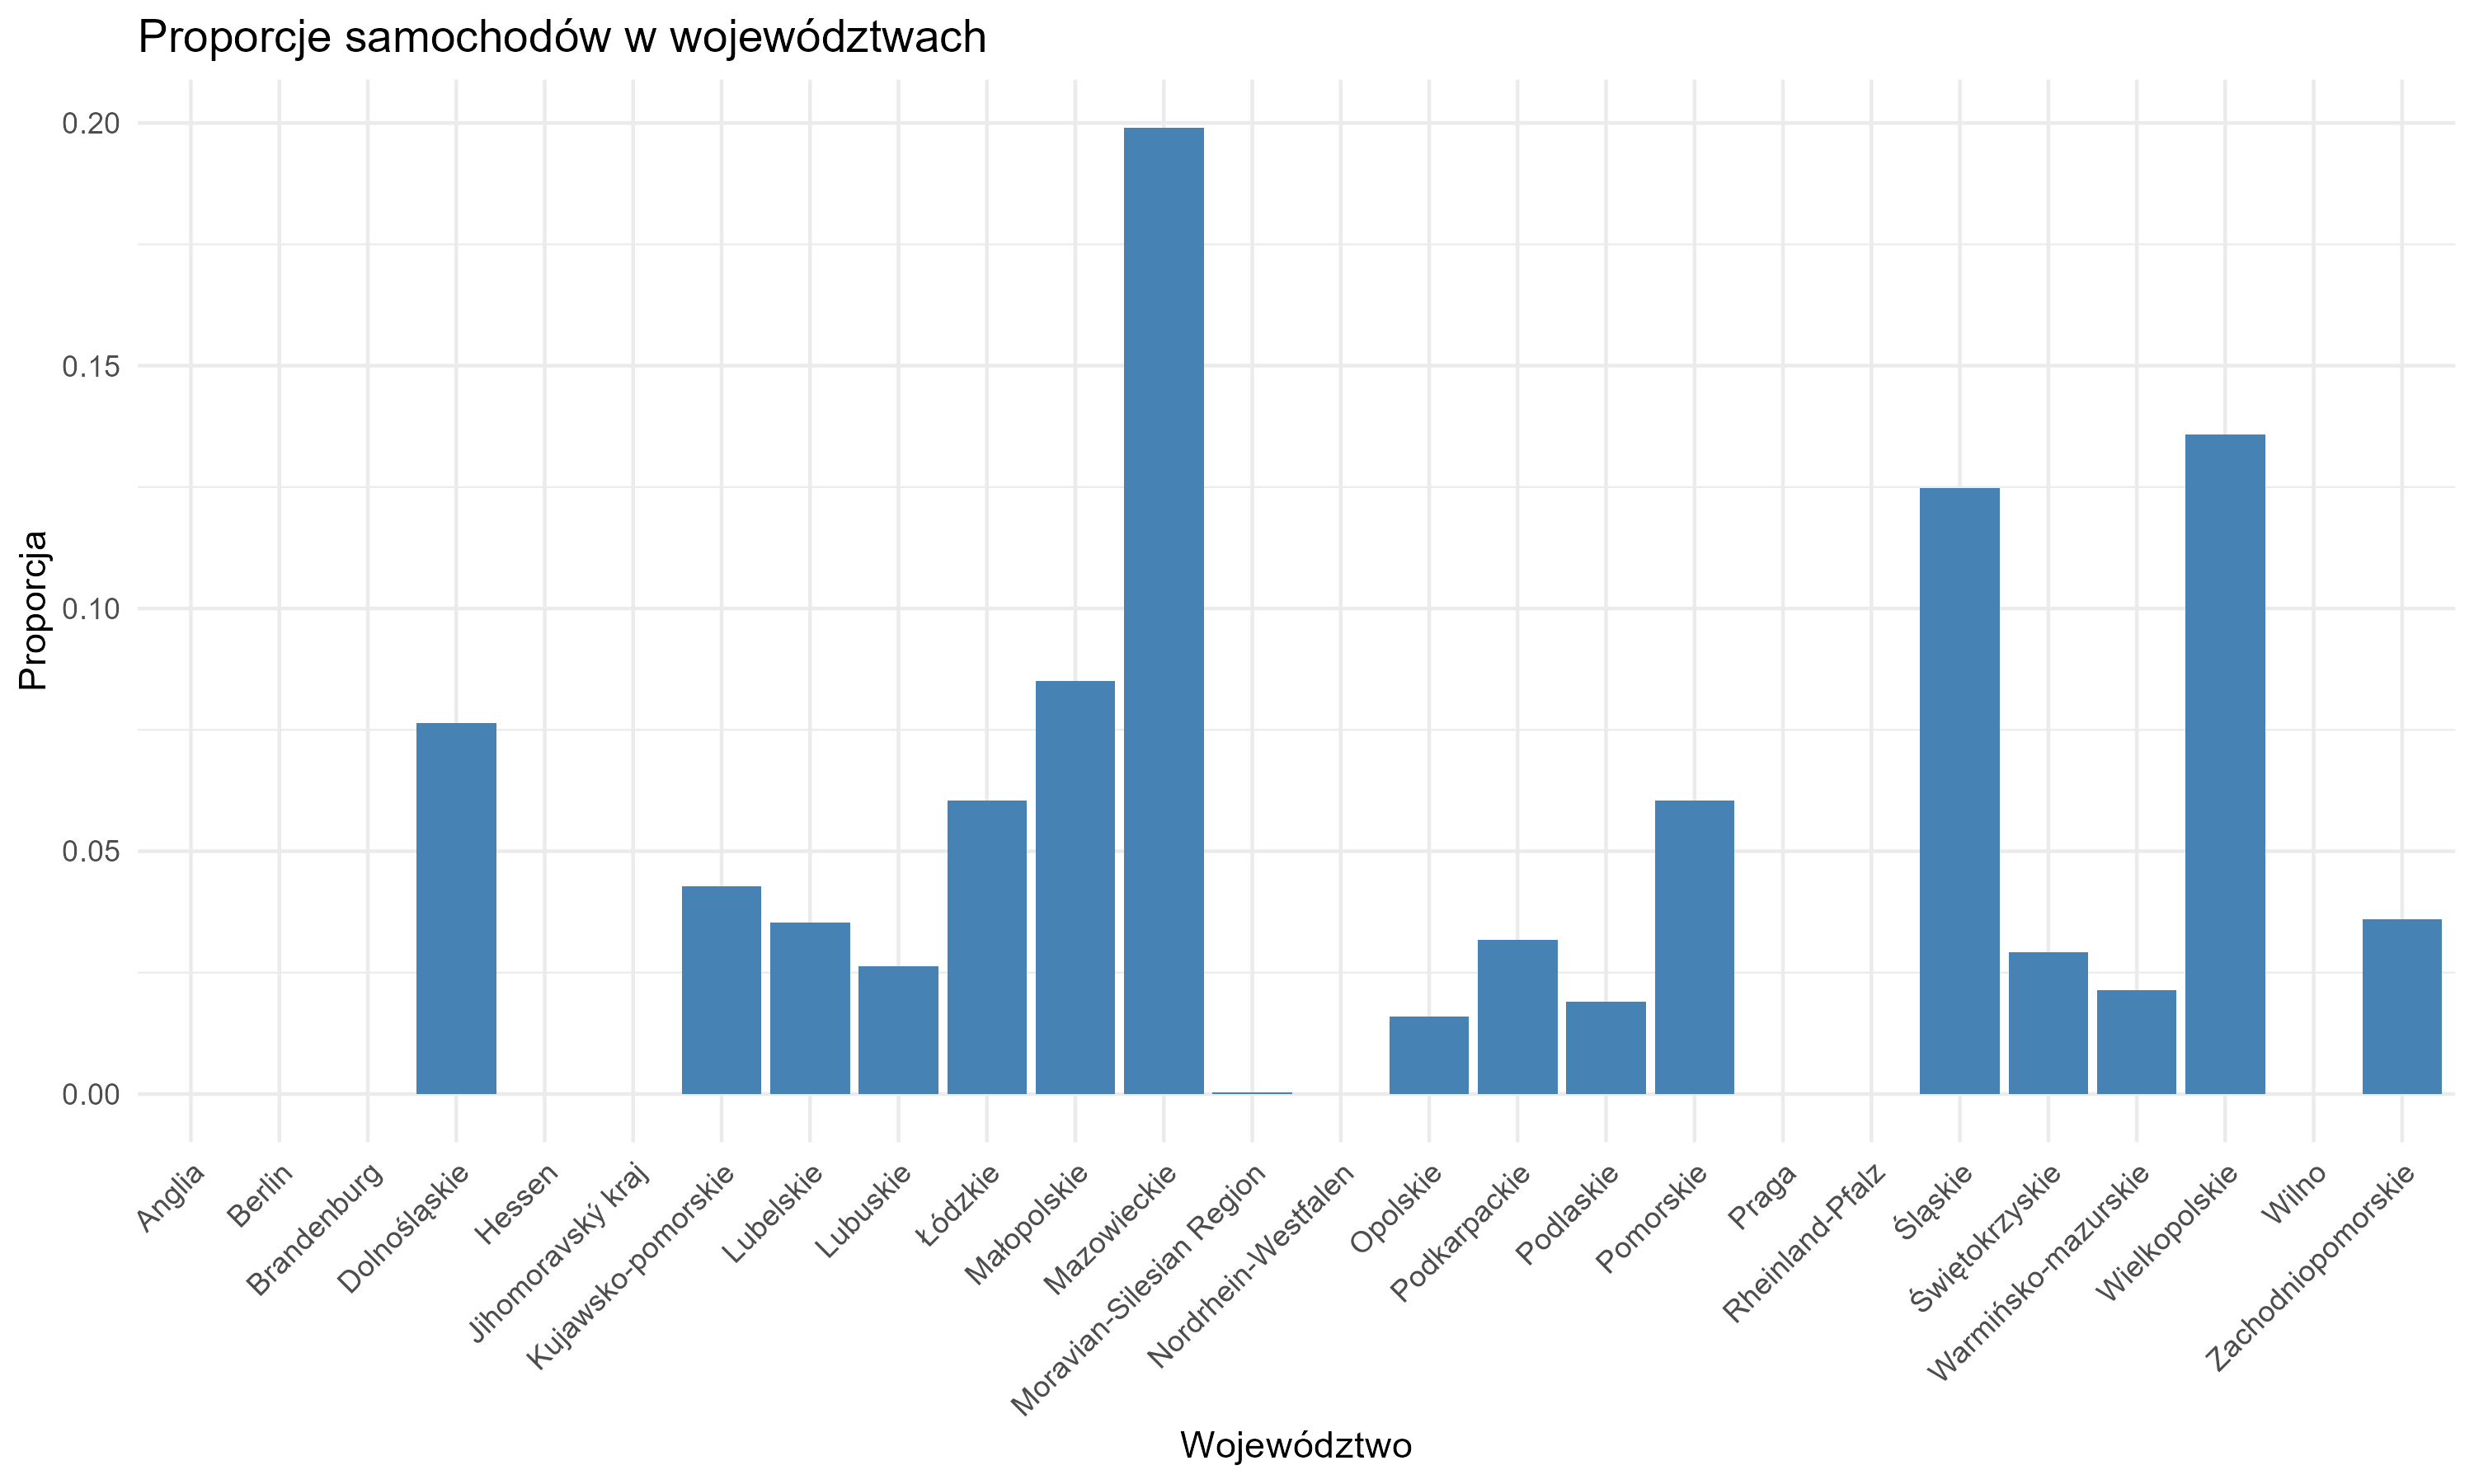
\includegraphics[width=1\linewidth]{analiza/wykres_proporcje}

Następnie oszacowaliśmy model regresji, żeby zbadać jak przebieg,
pojemność silnika, rok, skrzynia biegów i rodzaj paliwa wpływają na
wartość samochodu oraz identyfikować istotne czynniki determinujące
cenę.

\begin{Shaded}
\begin{Highlighting}[]
\CommentTok{\# 7. Regresja liniowa i korelacja}
\CommentTok{\# Regresja liniowa: Cena jako funkcja przebiegu, pojemności silnika i roku produkcji}
\NormalTok{model }\OtherTok{\textless{}{-}} \FunctionTok{lm}\NormalTok{(cena\_zl }\SpecialCharTok{\textasciitilde{}}\NormalTok{ przebieg\_w\_km }\SpecialCharTok{+}\NormalTok{ poj\_silnika }\SpecialCharTok{+}\NormalTok{ rok }\SpecialCharTok{+}\NormalTok{ skrzynia\_biegow}
            \SpecialCharTok{+}\NormalTok{ paliwo, }\AttributeTok{data =}\NormalTok{ dane)}
\FunctionTok{summary}\NormalTok{(model)}
\end{Highlighting}
\end{Shaded}

Model nie jest najlepiej dopasowanym modelem, o czym świadczy statystyka
R2, która wynosi 0,3767. Model wyjaśnia tylko 37\% wariancji ceny.
Analizując opracowany model regresji, możemy stwierdzić, że większość
zmiennych są istotne statystycznie na poziomie istotności 0,05. Żeby
lepiej wyjaśnić model, do modelu regresji dodamy zmienną marka oraz
wojewodztwo.

\begin{Shaded}
\begin{Highlighting}[]
\NormalTok{model }\OtherTok{\textless{}{-}} \FunctionTok{lm}\NormalTok{(cena\_zl }\SpecialCharTok{\textasciitilde{}}\NormalTok{ przebieg\_w\_km }\SpecialCharTok{+}\NormalTok{ poj\_silnika }\SpecialCharTok{+}\NormalTok{ rok }\SpecialCharTok{+}\NormalTok{ skrzynia\_biegow}
            \SpecialCharTok{+}\NormalTok{ paliwo }\SpecialCharTok{+}\NormalTok{ marka }\SpecialCharTok{+}\NormalTok{ wojewodztwo, }\AttributeTok{data =}\NormalTok{ dane)}
\FunctionTok{summary}\NormalTok{(model)}
\end{Highlighting}
\end{Shaded}

Powyższy model lepiej wyjaśnia zmiany cen, statystyka R2 = 0,5111. W tym
modelu zmienne odpowiadające nazwom województwa nie są istotne
statystycznie. Interpretacja zmiennych:\\
Każdy dodatkowy kilometr obniża cenę o 0.1946 zł. Każdy dodatkowy rok
zwiększa cenę średnio o 5,142 zł. Samochody z manualną skrzynią biegów
są średnio tańsze o 27,550 zł. Jest dużo wartości odstających, co
wymagałoby kolejne przetwarzania zmiennych: logarytmowania i
różnicowania zmiennych.

\begin{Shaded}
\begin{Highlighting}[]
\CommentTok{\# Wizualizacja regresji dla przebiegu}
\NormalTok{regresja }\OtherTok{\textless{}{-}} \FunctionTok{ggplot}\NormalTok{(dane, }\FunctionTok{aes}\NormalTok{(}\AttributeTok{x =}\NormalTok{ przebieg\_w\_km, }\AttributeTok{y =}\NormalTok{ cena\_zl)) }\SpecialCharTok{+}
  \FunctionTok{geom\_point}\NormalTok{(}\AttributeTok{alpha =} \FloatTok{0.5}\NormalTok{) }\SpecialCharTok{+}
  \FunctionTok{geom\_smooth}\NormalTok{(}\AttributeTok{method =} \StringTok{"lm"}\NormalTok{, }\AttributeTok{color =} \StringTok{"blue"}\NormalTok{) }\SpecialCharTok{+}
  \FunctionTok{labs}\NormalTok{(}\AttributeTok{title =} \StringTok{"Regresja: Cena a przebieg"}\NormalTok{, }\AttributeTok{x =} \StringTok{"Przebieg (w milach)"}\NormalTok{, }\AttributeTok{y =} \StringTok{"Cena (zł)"}\NormalTok{) }\SpecialCharTok{+}
  \FunctionTok{theme\_minimal}\NormalTok{()}
\FunctionTok{ggsave}\NormalTok{(}\StringTok{"regresja\_cena\_przebieg.png"}\NormalTok{, }\AttributeTok{plot =}\NormalTok{ regresja, }\AttributeTok{width =} \DecValTok{8}\NormalTok{, }\AttributeTok{height =} \DecValTok{6}\NormalTok{, }\AttributeTok{dpi =} \DecValTok{300}\NormalTok{)}
\end{Highlighting}
\end{Shaded}

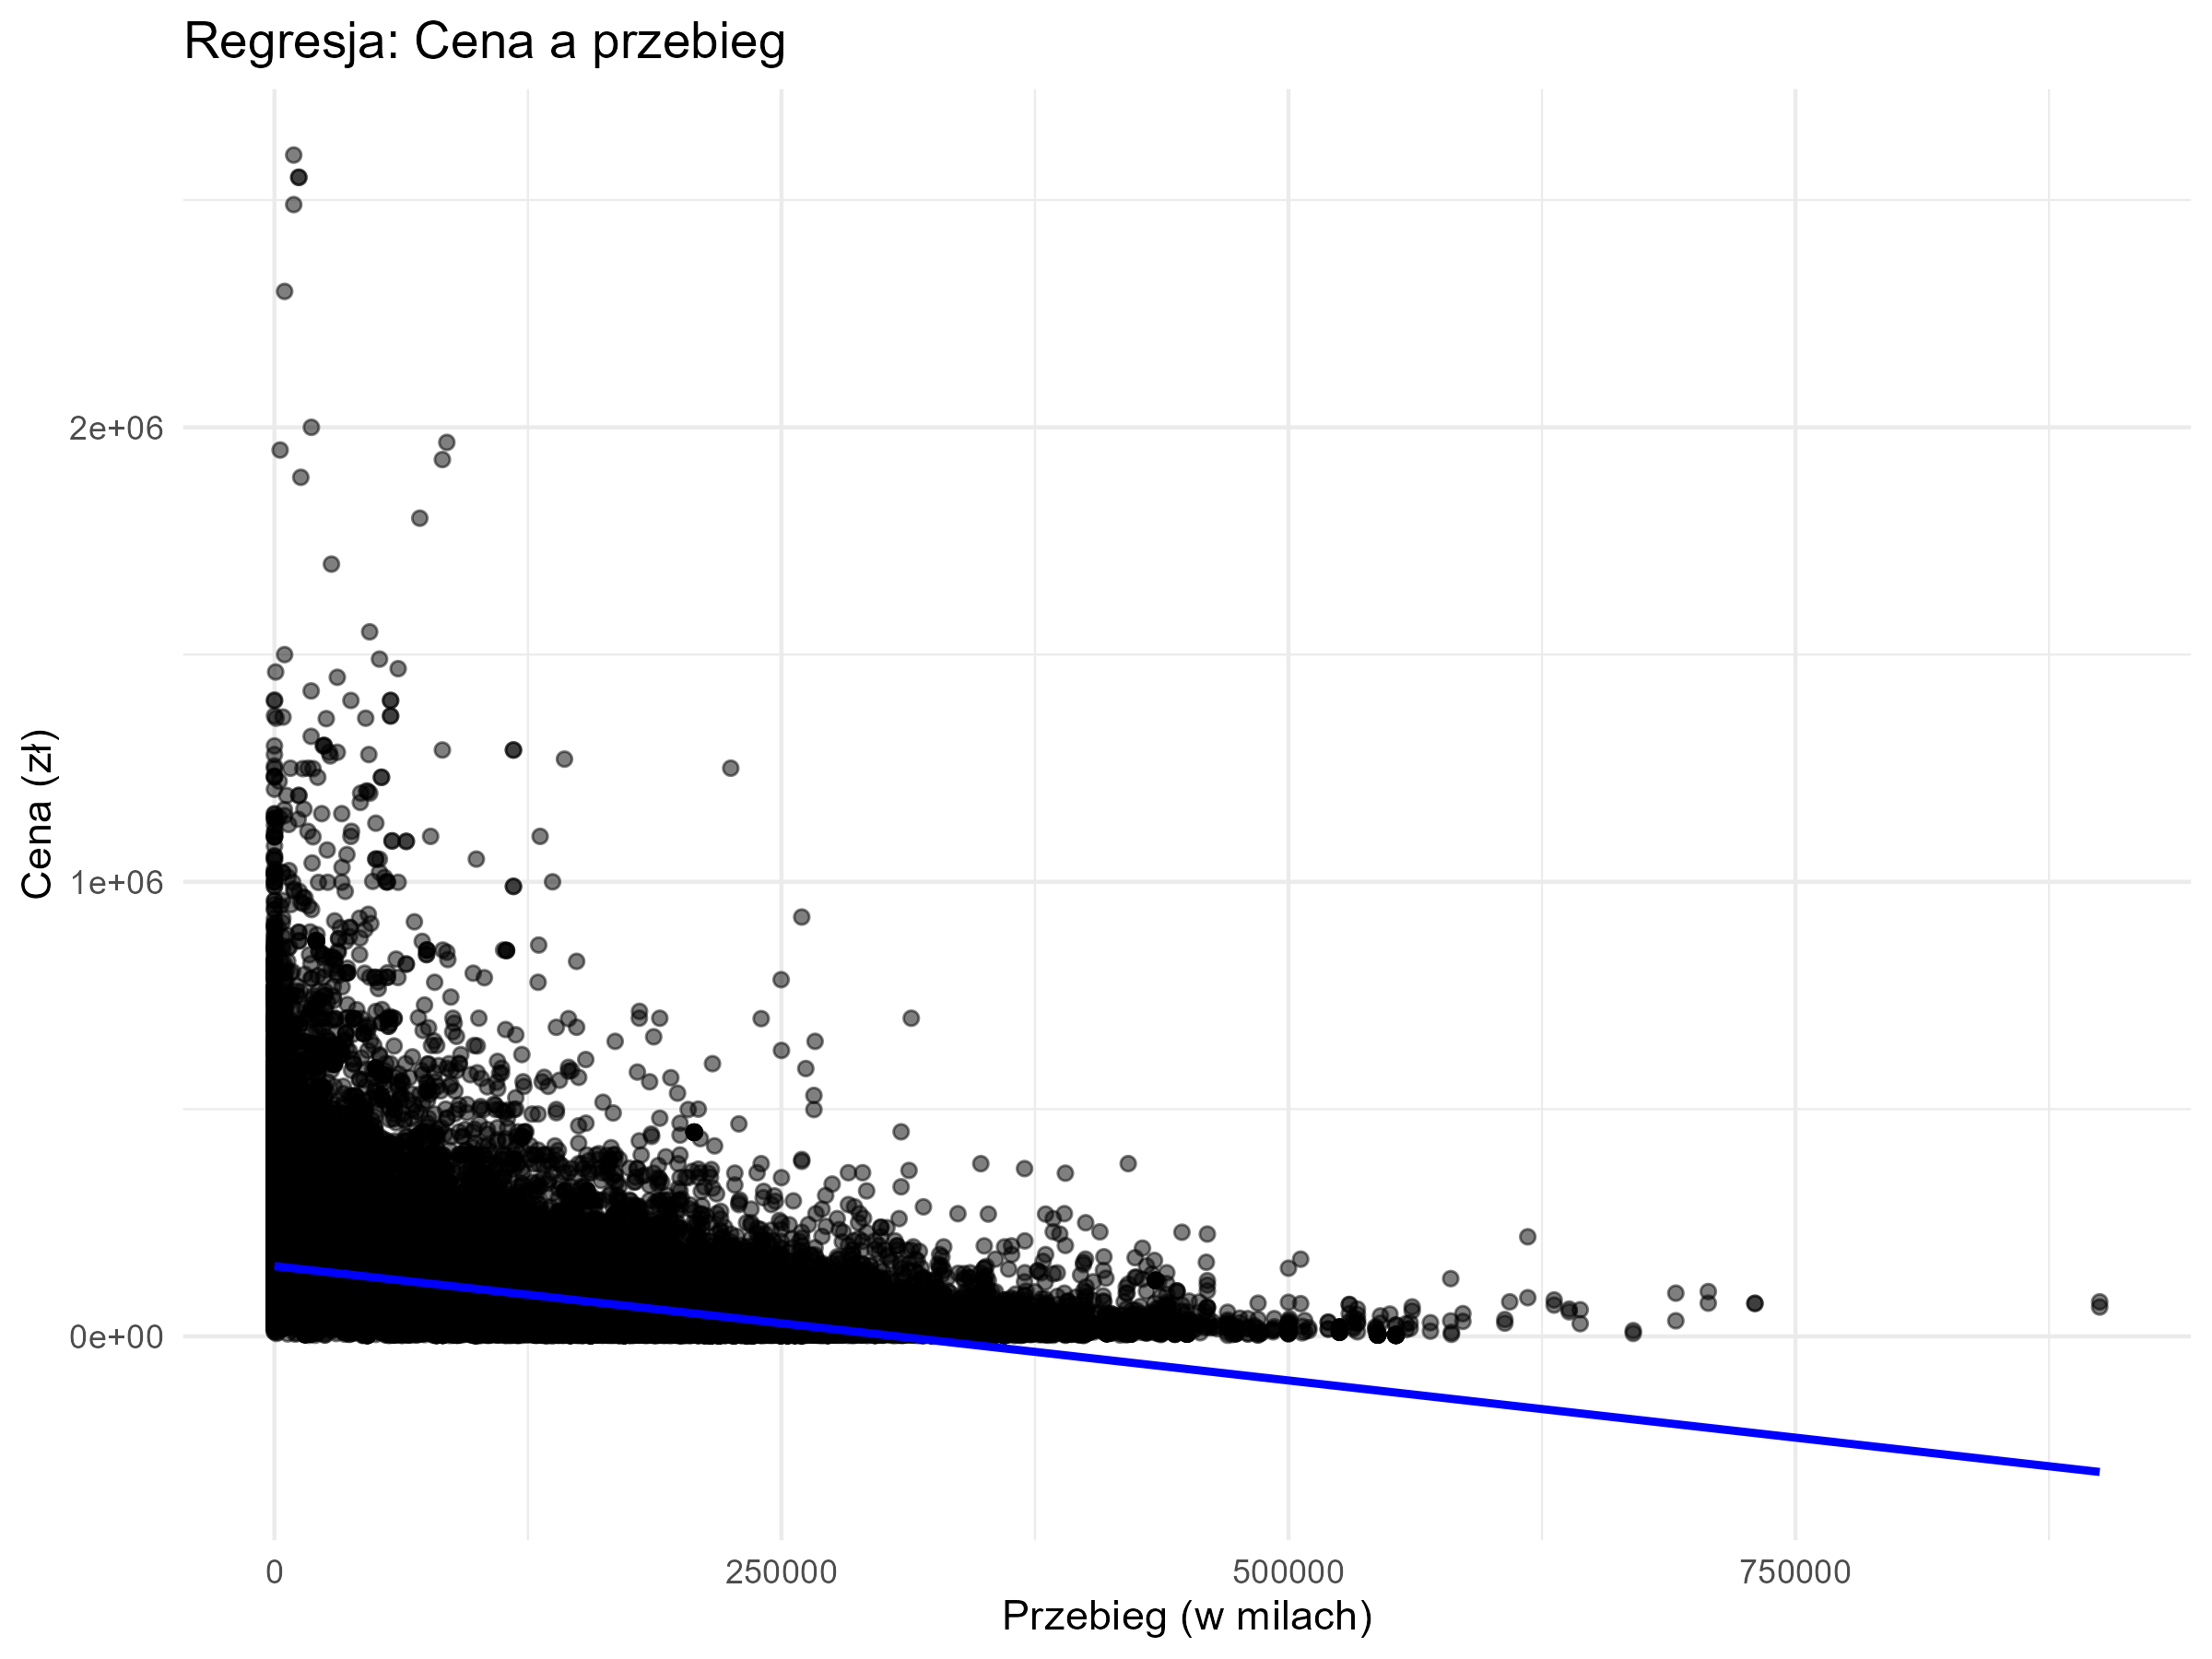
\includegraphics[width=1\linewidth]{analiza/regresja_cena_przebieg}

W celu określenia siły i kierunku zależności pomiędzy zmiennymi,
przeprowadziliśmy test korelacji na przykładzie zmiennych cena oraz
przebieg\_w\_km

\begin{Shaded}
\begin{Highlighting}[]
\NormalTok{correlation }\OtherTok{\textless{}{-}} \FunctionTok{cor.test}\NormalTok{(dane}\SpecialCharTok{$}\NormalTok{cena\_zl, dane}\SpecialCharTok{$}\NormalTok{przebieg\_w\_km, }\AttributeTok{use =} \StringTok{"complete.obs"}\NormalTok{)}
\FunctionTok{print}\NormalTok{(correlation)}
\end{Highlighting}
\end{Shaded}

Wskaźnik r= - 0.44 świadczy o ujemnej korelacji między ceną a
przebiegiem. Oznacza to, że im większy przebieg, tym niższa cena, ale
związek nie jest bardzo silny.

\subsection{Podsumowanie}\label{podsumowanie}

Przeprowadzona analiza opisowa pozwoliła na lepsze zrozumienie struktury
danych oraz ich potencjalnego wykorzystania. Analiza wykazała, że
najwięcej ofert dotyczy marki Volkswagen, a najmniej -- Lamborghini.
Najczęściej występującym paliwem jest benzyna i diesel, podczas gdy
pojazdy z napędem wodorowym prawie nie występują na portalu. Wykresy i
tabele liczności pozwoliły także określić dominujące województwa i
miasta pod względem liczby ofert. Testy statystyczne wykazały istotne
zależności między niektórymi zmiennymi.Przeprowadzona analiza korelacji
ujawniła, że na cenę samochodu największy wpływ mają rok produkcji i
przebieg, natomiast pojemność silnika ma relatywnie niewielkie
znaczenie. Testy statystyczne, w tym test chi-kwadrat, potwierdziły
istotne zależności między marką a województwem oraz rodzajem paliwa a
typem skrzyni biegów. Test proporcji wykazał znaczące różnice w
rozkładzie liczby samochodów w różnych województwach, co sugeruje
nierównomierne rozmieszczenie ofert sprzedaży w Polsce. Może to wynikać
z różnic w poziomie urbanizacji i zamożności mieszkańców poszczególnych
regionów. Analiza korelacji pokazała, że cena samochodu jest
umiarkowanie skorelowana z rokiem produkcji i słabo z pojemnością
silnika, natomiast wykazuje silną ujemną korelację z przebiegiem.
Podsumowując, nowsze samochody są droższe, a większy przebieg obniża ich
wartość, co jest zgodne z intuicyjnymi założeniami rynkowymi. Dodatkowo,
bardzo słaba korelacja pojemności silnika z ceną może sugerować, że inne
czynniki, takie jak marka czy wyposażenie, mają większy wpływ na wartość
pojazdu. Regresja liniowa potwierdziła istotność takich zmiennych jak
rok produkcji, przebieg oraz rodzaj skrzyni biegów w kształtowaniu ceny
pojazdu. Początkowy model wyjaśniał 37\% wariancji cen, jednak po
dodaniu marki i województwa jego skuteczność wzrosła do 51\%. Wyniki te
wskazują, że czynniki lokalizacyjne i preferencje marek również wpływają
na wartość samochodu. Wnioski płynące z analizy mogą być przydatne
zarówno dla sprzedających, jak i kupujących, umożliwiając lepsze
przewidywanie wartości rynkowej pojazdów.

\end{document}
